\chapter{制冷}
\section{引言}
制冷对超导非常重要。对制冷的依赖性是超导广泛应用(如电力应用)的主要因素。然而,我们不以因为其重要性而过分强调它的作用。
单从制冷角度看,显然将超导磁体运行于最高的许可温度下是更高效的。但是,如果超导磁体是某系统的一部分,就必须评估运行温度对整个系统的影响。
“超导磁体的最佳运行温度”这个问题就成了现实且极端重要的设计/运行问题,对高温超导磁体尤其如此。比如,对运行于77 K的超导磁体,如果产生
相同的磁场,无疑需要比运行于20 K更多的超导体;制冷上的节省可能并不能补偿超导体费用的增加。

另一个不可忽略的是每一个超导系统的绝热要求:最好的绝热是真空。温度低于20 K(氢的冰点)时,热学“有效”的真空在低温容器内是相对容易实现的。
已抽真空的低温容器表面逸出的氢气是容器内最主要的传热介质。于是,整个高温超导磁体系统若运行于20 K之下(而不是之上)可能经济性更好。
如果我们选择一个更高的运行温度——比如很多人希望的~70 K——系统中可能不再需要真空绝热,这时“干扰”又少了一点。

本部分,将简要讨论以下超导磁体的制冷设计、运行问题:1)两种超导体的冷却方式,“干式”和“湿式”;2)冷源、热源和制冷测量;
3)湿式磁体的制冷剂;4)可能对干式磁体有用的固体制冷剂。上述论题的更多细节将在“专题”部分有更深入的涉及和研究。

\section{“湿式”磁体和“干式”磁体}
在1990s前,所有的超导磁体都是“湿式”的,即靠液氦冷却。1990s早期开的,随着高温超导的发现以及制冷机技术的进步,由制冷机冷却的干式(无制冷剂)
LTS和HTS磁体都得以发展。一方面,干式低温系统在运行、维护上更轻便;另一方面,干式低温系统更易实现“少干扰”。这使得干式磁体在多数应用中是更优的
选项——如果磁体自身在正常运行条件下完全无耗散(如交流损耗)的话。

\subsection*{超导磁体的冷却方式}
如表4.1可见,超导磁体可以使用五种冷却方式(四种湿式和一种湿式)的任一种。尽管本节使用的“制冷??”、“绝热”、“准稳定性”等术语
在第六章会有更详细的讨论,但为了读者的可理解性,此处给出这些术语的简要定性解释。
\begin{description}
  \item[浸泡冷却cryostable?] 1980s以前建造的磁体基本都是浸泡式冷却的。这些磁体的一个关键制冷特征是为了便于制冷剂渗入的绕组的“通孔”设计。
  通孔让绕组的几乎所有部分都暴露于制冷工质。此时,下文定性讨论的对流传热是重要的。第六章会给出一些数据。
  \item[浸泡冷却绝热] 为了实现高性能,浸泡冷却的“绝热”磁体在1980s早期开始发展。此处,绕组是实心的,完全没有制冷剂的浸入。
  这样,绕组中的总体电流密度显著高于浸泡制冷??。绕组仅在其外表面被冷却。
  \item[迫冷cryostable] 为了保持制冷剂为单相(一般对浸泡式制冷磁体并不容易),以及为了加强绕组导体本身的强度,在1970s早期发展了所谓的“cable-in-conduit,CIC,特别是大型磁体”。此处,冷却和绕组高度耦合。重要的传热数据是哪些强迫对流参数。典型的传热数据在第六章给出。
  \item[迫冷准稳定性] 为了保持绕组鲁棒性,绕组上没有通孔。为实现比浸泡冷却绝热磁体更好的稳定性,制冷剂被强迫进入绕组。不是经由导体,而是
  仅在导体的临近边缘。和绝热绕组一样,导体是传导冷却的。
  \item[制冷机冷却] 磁体和制冷机相连;绕组内的冷却主要通过传导。如第六章将会更详细讨论的,LTS磁体运行于准稳定态,而HTS磁体运行于稳定态。
  “制冷循环器(cryocirculator)”对作为干式磁体冷源的制冷机是非常需要的,特别是对LTS磁体。
\end{description}
%%%表4.1
\begin{table}[htbp]\small
  \centering
  \caption{湿式和干式超导磁体的冷却方式} \label{coolingmethod}
\begin{tabular}{|c|c|c|}
  \hline
  % after \\: \hline or \cline{col1-col2} \cline{col3-col4} ...
\textbf{冷却方式}&\textbf{冷却-导体耦合性}&\textbf{传热方式} \\ \hline \hline
浸泡冷却,cryostable & 好;全部导体& 对流\\ \hline
浸泡冷却,绝热 & 基本不存在 &(磁体绕组表面的)传导 \\ \hline
迫冷,cryostable &好;全部导体&对流\\ \hline
迫冷,准稳定 &临近表面处,间接&传导\\ \hline\hline
制冷机,准稳定&间接 &传导 \\ \hline
\end{tabular}
\end{table}

\section{制冷问题:冷却、热、测量}
三个基本制冷问题是与超导磁体技术相关的:1)冷源;2)热源;3)测量。这些问题将在本部分简要讨论。专题部分以及后续章节将对某些特定问题
做更详细的讨论。
\subsection{冷源}
如表4.1总结的,超导磁体靠制冷工质或制冷机冷却并维持在其运行温度。下面将简明的讨论制冷剂。制冷机仅给出基本的热力学关系和性能数据。
\subsection{热源}
一般的,在超导磁体的低温容器内的冷环境中,主要有五个热源:1)低温容器壁间的辐射;2)低温容器壁间“真空”空间的热对流;3)磁体支撑和
低温容器结构单元的热传导;4)电流引线的传导和焦耳热耗散;5)磁体内的耗散。专题部分将会涉及到辐射、对流和电流引线。磁体的耗散将在第七章讨论。
\subsection{测量}
超导磁体运行中,通常测量的低温参数包括:1)温度;2)压力(低温容器真空度、工质压力);3)工质流速(迫冷湿式磁体);4)蒸发率(湿式磁体的电流引线)。本书中,专题部分仅涉及温度的测量简要讨论。

\section{液体工质:湿式磁体}
1990s前,仅液氦适用于磁体运行。某些液氦低温容器使用液氮来隔断热量。由于磁体要从室温冷却到4.2 K,液氮也用于预冷液氦冷却磁体,以减少液氦的消耗。

大气压下饱和(沸腾)温度低于100K的6种工质是:氧(90.18 K)、氩(87.28 K)、氮(77.36 K)、氖(27.09 K)、氢(20.39 K)、氦(4.22 K)。
对于湿式高温超导磁体和设备,工质的备选顺序为氮、氖、氢。对于湿式低温超导或低温/高温混合磁体,如高场NMR磁体,仍然主要使用氦。五种
液体的沸腾热传递参数在表4.2列出。作为对比,还列出了水的参数。

%%表4.2
\begin{table}[htbp]\small
  \centering
  \caption{沸腾传热参数} \label{boilingpara}
\begin{tabular}{|c||c|c|c|c|c|}
  \hline
  % after \\: \hline or \cline{col1-col2} \cline{col3-col4} ...
\textbf{液体}&$T_a[K]$&$h_l[J/cm^3]$&$q_{pk}[W/cm^2]$&$\Delta T_{pk}[K]$&$q_{fm}[W/cm^2]$ \\ \hline \hline
氦&4.22&2.6&$\sim 1$&$\sim 1$&$\sim 0.3$\\ \hline
氢&20.39&31.3&$\sim 10$&$\sim 5$&$\sim 0.5$ \\ \hline
氖&27.09&104&$\sim 15$&$\sim 10$&$\sim 1$\\ \hline
氮&77.36&161&$\sim 25$&$\sim 15$&$\sim 2$\\ \hline
水&373.15&2255&$\sim 100$&$\sim 30$&$\sim 10$ \\ \hline
\end{tabular}
\end{table}

\subsection*{沸腾传热参数}
在湿式超导磁体中,特别是浸泡冷却cryostable磁体,冷却依靠核态沸腾传热。由于核态沸腾传热中,冷却是靠液体蒸发实现的,故液体的体积蒸发热$h_l$
是一个关键参数。这也意味着沸腾热流密度和温度的关系图像(两坐标轴均为对数坐标,如图\ref{boilingflux})对大多数液体都是看上去类似的。这里的x轴温度是浸入
液体的物体的避免温度和液体饱和温度之差,即$\Delta T=T-T_s$。图中的其他参数为:$q_{pk}$,最大核态沸腾热流密度;$\Delta T_{pk}$,是$q_{pk}$出现时的$\Delta T$;$q_{fm}$,最小膜态沸腾热流密度。

从表\ref{boilingpara}中我们可以得到,唯一适合LTS磁体的制冷剂液氦,蒸发时吸收的能量密度最小,是效果最差的。尽管HTS磁体最好是干式运行,但如果它湿式运行,
氢、氖、氮能够覆盖大多数HTS磁体的温度范围。燃料电池在电动汽车领域应用中发展出的一个重要成果就是液氢技术,包括安全性方面的技术。这可能会为
液氢冷却HTS磁体提供与有益促进。

%%%图4.1
\begin{figure}
  \centering
 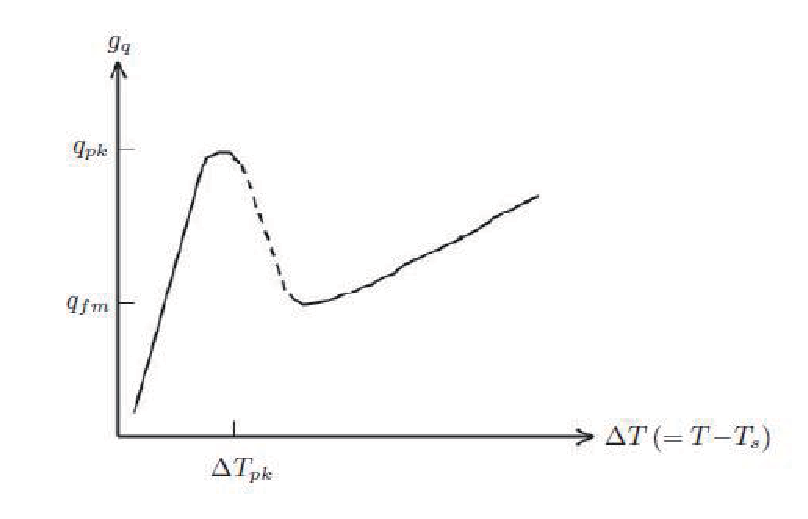
\includegraphics[scale=0.8]{chpt4/figs/fig4.1.eps}
  \caption{典型流体的沸腾热流密度 vs. 温度}\label{boilingflux}
\end{figure}

\section{固体工质:干式磁体}
正如前文所讲,干式低温磁体,特别是运行电流小于1 kA的,很可能会逐渐替代湿式小电流LTS磁体。如果当前的高温超导体(BSCCO、YBCO和$MgB_2$)中
的一种、两种甚至三种发展为完全的“磁体级导体”,那在不久的将来,干式HTS磁体不仅会取代干式LTS磁体,还将找到仅适用于HTS磁体的其他应用。
\subsection{湿LTS磁体 vs. 干HTS磁体——热容}
湿式LTS磁体经常被忽略的一个优势是其巨大的热容,这是由作为湿式LTS磁体的一部分的大量液氦提供的。液氦的焓密度在4.2 K时“高”达$2.6 J/cm^3$——
此处所谓高,是和铜相比的。铜在4.2-4.5 K的焓密度仅为$\sim 0.0003J/cm^3$——是铜的1000倍。于是,在大多数情况下,液氦将牢牢将磁体的温度“铆”住。

干式磁体同样需要提供一个大的热容以便“铆”住温度。固态制冷剂是这种功能的很好选项。图\ref{fig:heatcap}给出了多种固体制冷剂(固氖、固氮、固氩)以及
部分金属(铅、银、铜)的热容和温度的关系。铅在低温设备中常用为热容增强部件;铜是LTS中广为使用的基底金属;银是BSCCO的基底金属。
%%%图4.2
\begin{figure}
  \centering
 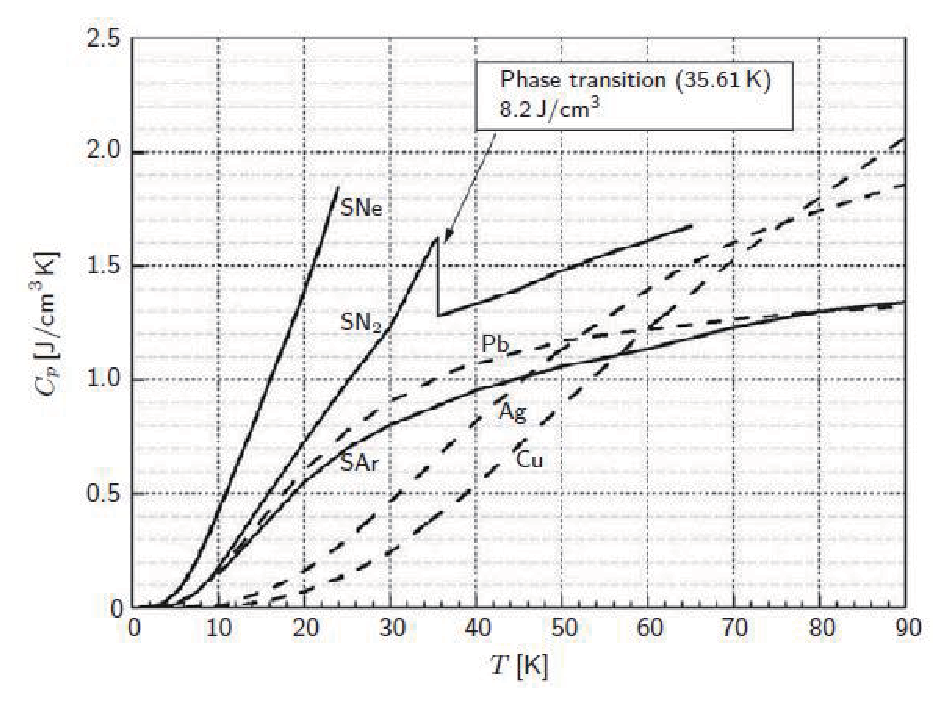
\includegraphics[scale=0.7]{chpt4/figs/fig4.2.eps}
  \caption{几种物质的热容$C_p$ vs. 温度T特性}\label{fig:heatcap}
\end{figure}

\subsection{固体工质——氖、氮、氩}
下面将简要讨论三种可能用于干式HTS磁体的固体工质:氖、氮、氩。附录中给出了他们的一些热力学性质。

尽管是高热容使得固体工质成为优秀的浸渍材料。此外,还有两个其他的性质让固体工质在一些应用中优于环氧:1)热导率;2)机械强度。在10-15 K温度区间,
在HTS绕组上的温度均匀性上,固氮比环氧的效果更好。同时,固氮也使得绕组比环氧浸渍更具鲁棒性。

\begin{description}
  \item[固氮,$SN_2$] 因为它能在高达64.2 K仍保持固态且不贵、重量很轻(铅的密度的1/10)、具有电绝缘性,固氮是运行于64 K温度下温区的干式HTS磁体的
  有效热容增强剂。例如,BSCCO和YBCO磁体在20-60 K温区肯定能运行;$MgB_2$磁体则是在10-15 K甚至20-30 K。从图4.2中看出,固氮在35.61 K存在一个
  固-固态的相变,额外吸收能量$8.2J/cm^3$。由于在转变点古今的热容是约$1.5J/cm^3 K$,额外的$8.2J/cm^3$能量吸收等价于5 K多的温升。对于运行于
  这个温区的HTS磁体,这是一个极佳的“温度池”。
  \item[固氖] 图4.2中的热容数据表明,固氖体积费用比固氮贵200倍,它将是4-10 K温区的最佳热容增强剂。不过,10K左右时,固氮对于大多数情况就足够用了。
  尽管也有其他物质,比如$Er_3 Ni$,在4-24 K温区能提供更好的热容增强效果。但是对磁体,固氖可能更合适。除了价格之外的最大缺点(相比于固氮),是
  固氖相对低的熔点,仅24.6 K。这限制了固氖系统运行的温区。
  \item[固氩] 作为大气中含量最高的惰性气体,氩在价格上比氖至少便宜 一个数量级,不过比氮还是贵不少。固氩仅适用于运行于64.2 K(固氮熔点)
  -83.8 K(固氩熔点)温区的干式磁体。
\end{description}

\section{专题}
\subsection{问题4.1:Carnot制冷机}
因为超导电性发生在很低温度,所以需要制冷机来实现并维持低温环境。
使用图4.3所示的Carnot制冷机,我们来研究用于制冷的最高效率的热力学过程。
Carnot制冷机由两个可逆绝热过程和两个可逆等温过程组成,工质流体在两个热源之间运行,
从而最高效率的做功。尽管Carnot效率实际中是不能实现的,但它给出了可能的上限。

a) 在$T$ vs. $S$图上画出Carnot循环。使用图4.3中标出的记号。$T_{op}$:冷源温度,一般等于磁体运行温度;
$S_{cl}$:离开冷源的工质的熵;$T_{wm}$:高温热源的温度;$S_{wm}$:进入高温热源的工质的熵。冷源和热源的温度$T_{op}$和$T_{wm}$都是常数。

b)证明,对于理想Carnot制冷机,为了从热源$T_{op}$中提取热量$Q$并将其释放到$T_{wm}$中,需要的输入功$W_{ca}$为:
\begin{equation}% 4.1
W_{ca}=Q(\frac{T_{wm}}{T_{op}}-1)
\end{equation}

c)证明,高温热源为$T_{wm}=300\ \mathrm{K}$的Carnot制冷机,在$T_{op}=4.2\ \mathrm{K}$时,$W_{ca}/Q\simeq 70$;
在$T_{op}=77\ \mathrm{K}$时,$W_{ca}/Q\simeq 3$。
\begin{figure}[htbp]
	\centering
	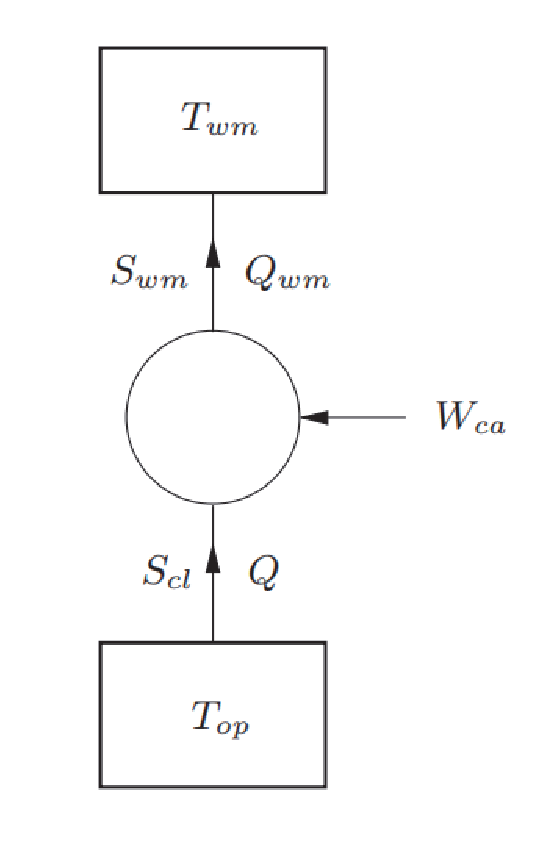
\includegraphics[scale=0.5]{chpt4/figs/fig4.3.eps}
	\caption{工作于两个热源之间的Carnot制冷机。}
\end{figure}

\subsubsection{问题4.1之解}
a) Carnot制冷机工作于两个热源之间,从低温热源$T_{op}$中提取热量$Q$,然后向高温热源$T_{wm}$释放热量$Q_{wm}$。
如图4.3所示,制冷机的运行需要功$W_{ca}$。

Carnot制冷循环由工质的四个可逆过程组成,如图4.4的$T$ vs. $S$图所示:
\begin{itemize}
	\item 工质的等熵压缩,开始于状态1($S_{wm},T_{op}$);
	\item 等温压缩,开始于状态2($S_{wm},T_{wm}$);
	\item 等熵膨胀,开始于状态3($S_{cl},T_{wm}$);
	\item 等温膨胀,开始于状态4($S_{cl},T_{op}$),结束于状态1。
\end{itemize}

b)热力学第一定律:
\begin{equation*}% S1.1
Q_{wm}=Q+W_{ca}=0 \tag{S1.1}
\end{equation*}

式中,$W_{ca}$是制冷机的输入功,等于$T$ vs. $S$图上的闭合面积(当图4.3中的$W_{ca}; Q; Q_{wm}$方向相反时,
Carnot循环代表理想做功机,$T$ vs. $S$图上的闭合面积表示输出功)。
因为每个过程都是可逆的,有$Q=T_{op}(S_{wm}-S_{cl})$和$Q_{wm}=T_{wm}(S_{wm}-S_{cl})$。有:
\begin{align*}% S1.2a
S_{wm}-S_{cl}&=\frac{Q}{T_{op}}\tag{S1.2a}\\
S_{wm}-S_{cl}&=\frac{Q_{wm}}{T_{wm}}\tag{S1.2b}
\end{align*}

令上面两个式子相等,有:
\begin{equation}% S1.3
\frac{Q}{T_{op}}=\frac{Q_{wm}}{T_{wm}} \tag{S1.3}
\end{equation}

联立S1.1和S1.3,有:
\begin{equation*}% S1.4
\frac{Q}{T_{op}}=\frac{Q+W_{ca}}{T_{wm}} \tag{S1.4}
\end{equation*}

解出S1.4中的$W_{ca}$,得到:
\begin{equation*}% 4.1
W_{ca}=Q(\frac{T_{wm}}{T_{op}}-1) \tag{4.1}
\end{equation*}

\begin{figure}[htbp]
	\centering
	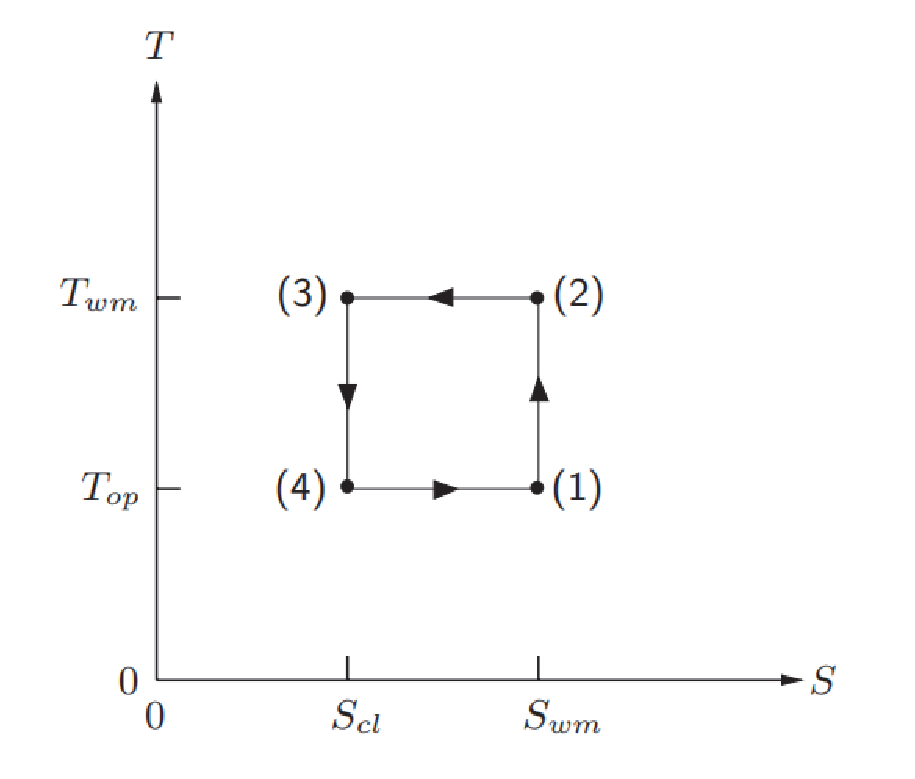
\includegraphics[scale=0.5]{chpt4/figs/fig4.4.eps}
	\caption{Carnot制冷机的$T$ vs. $S$图。}
\end{figure}

c)\textbf{$4.2–300\ \mathrm{K}$温区}:在$T_{op} = 4.2\ \mathrm{K}, T_{wm} = 300\ \mathrm{K}$
时,从方程4.1可得$W_{ca}/Q\simeq 70$;也就是说,4.2 K的1 W制冷量,需要制冷机70 W的输入功。
实际制冷机中,性能比定义为$W_{ca}/Q$($W_{cp}$是压缩功)随着$Q$增大而提高。
小单元($Q=1\ \mathrm{W}$)大概$\sim 10,000$,大单元($Q\sim 100\ \mathrm{kW}$)在$\sim 300$。

\textbf{$7.7–300\ \mathrm{K}$温区}:将$T_{op} = 77\ \mathrm{K}, T_{wm} = 300\ \mathrm{K}$
代入方程4.1,可得$W_{ca}/Q\simeq 3$;实际制冷机性能比在$\sim 50$(小单元,$1\ \mathrm{W}$)到$\sim 10$(大单元,$\sim 100\ \mathrm{kW}$)之间。

\subsection{讨论4.1:制冷机性能}
这里,我们简要从两个不同的角度看一下制冷机的性能:
1) 单一额定功率下的制冷机在不同运行温度下($Q/T_{op}$);
2) 组合额定功率下和运行温度,但运行在不同温度下。

\textbf{A. 特定温度下的特定制冷功率}

图4.5给出的是特定制冷功率$Q$($\mathrm{W}$)下的$W_{cp}/Q$ vs. $T_{op}$关系曲线[4.19]。
图中的$\otimes$符号表示Carnot循环。
\begin{figure}[htbp]
	\centering
	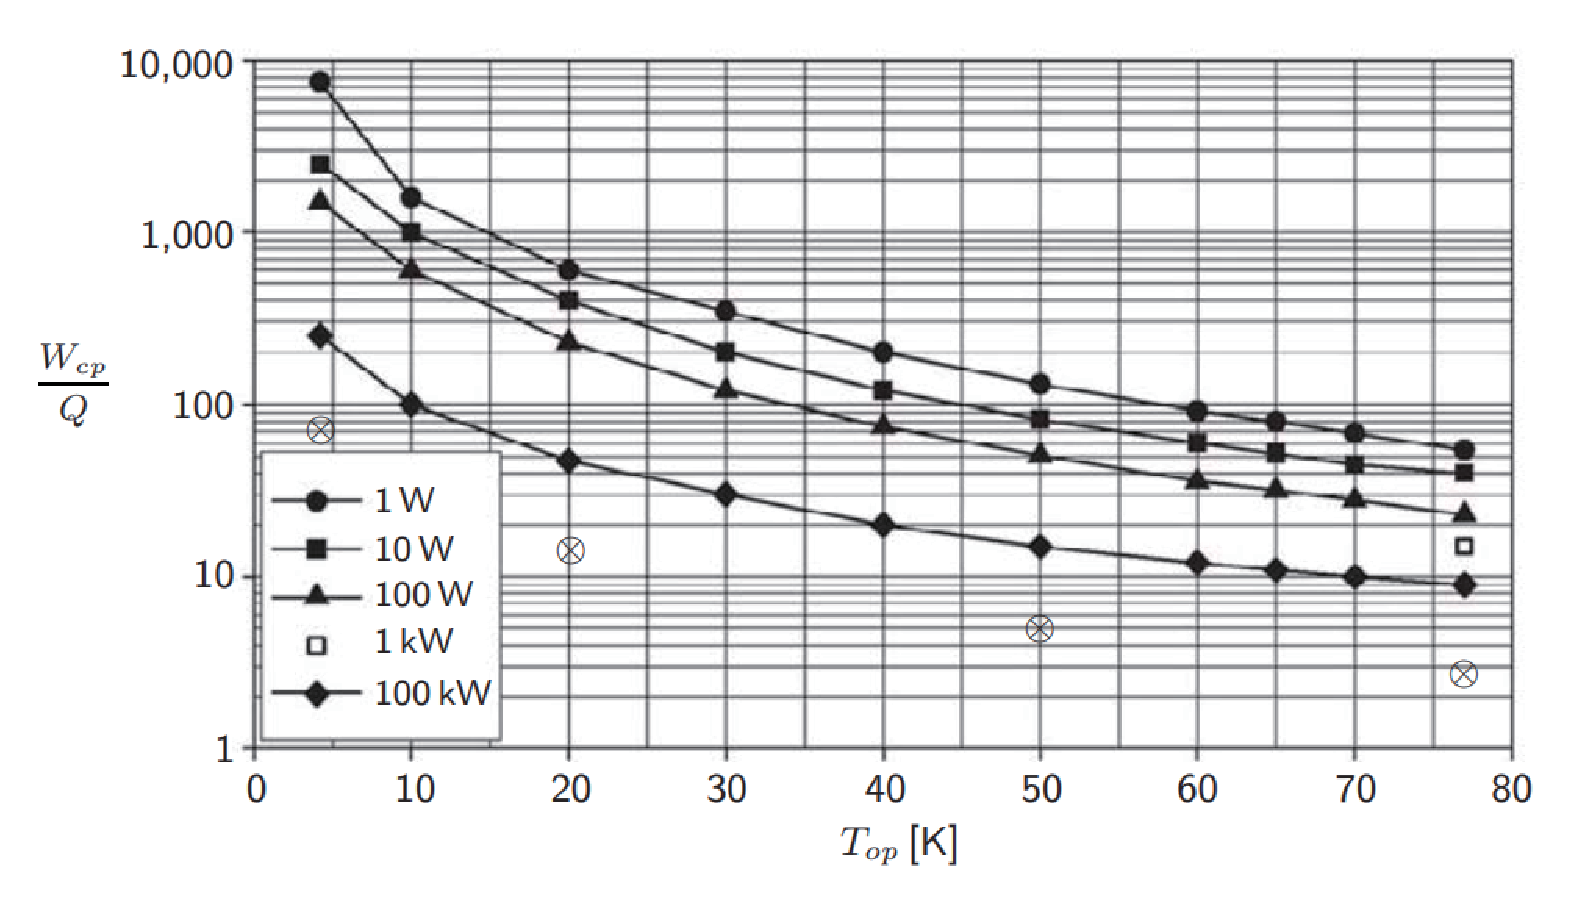
\includegraphics[scale=0.4]{chpt4/figs/fig4.5.eps}
	\caption{特定制冷功率$Q$($\mathrm{W}$)下的$W_{cp}/Q$vs. $T_{op}$关系曲线。$\otimes$符号表示选定温度下的Carnot循环,计算时取$T_{wm}=300\ \mathrm{K}$。}
\end{figure}

这样,对一个设计运行温度$T_{op}=4.2\ \mathrm{K}$的1 W制冷机(实心圈)的$W_{cp}/Q$是7500;
对运行温度$T_{op}=20\ \mathrm{K}$的1 W制冷机,$W_{cp}/Q$是600。
下面将论及,在特定温度4.2 K和20 K下优化的制冷机在不同温度区间$T_{op}$下的$W_{cp}/Q$是不同的。

\textbf{B.在非设计温度下的运行}

\begin{figure}[htbp]
	\centering
	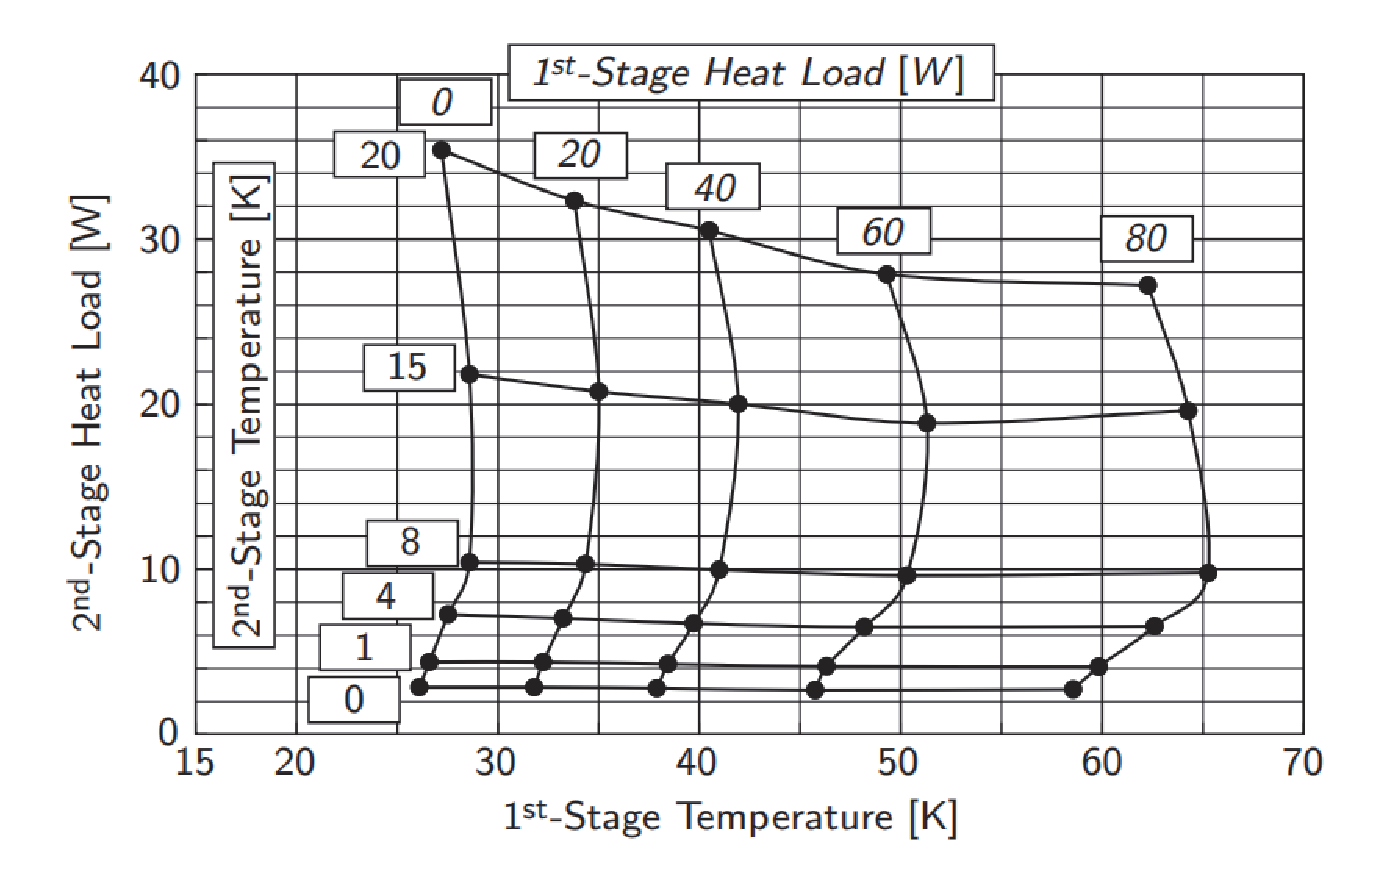
\includegraphics[scale=0.5]{chpt4/figs/fig4.6.eps}
	\caption{二级制冷机的性能数据。}
\end{figure}

图4.6给出了一台二级制冷机(住友重工Model RDK-408D2)的性能(一、二级制冷功率)数据,
性能是作为第一级和第二级运行温度的函数给出的。
它的标称最低二级运行温度是4.2 K,此时的制冷功率$Q=1\ \mathrm{W}$需要压缩功率$W_{cp}=7.5\ \mathrm{kW}$,
也即$W_{cp}/Q = 7500$。数据给出了制冷机在同样的压缩功率下的二级功率/温度比:从3 K时的0W,即$W_{cp}/Q = \infty$,到
20 K时的15 W,即$W_{cp}/Q = 500$。 (图4.5表明,一个15 W/20 K单元在20 K优化后的$W_{cp}/Q$大约是350。)
那些在给定二级温度为大约20 K时近乎水平的二级制冷线表明,在一级温度处于$\sim 25-\sim 60\ \mathrm{K}$区间时二级制冷功率几乎与之无关。

因为制冷机的压缩功率7.5 kW与一二级负荷无关,为了维持二级温度在一个理想水平,
总的热负荷,至少是二级的热负荷,必须匹配其制冷功率。
这样,如果二级运行温度希望是20 K——一级运行条件为 40 W/42 K——如果二级的实际热负荷是5 W,
那必须给二级提供额外的10 W的热负荷。因为如图4.6所示,二级在20 K提供15 W的制冷功率。
这个额外的10 W热负荷一般由附属于二级冷头的加热器产生,这会导致系统效率的降低。


\subsection{讨论4.2:湿磁体的冷却模式}
因为从体积上讲,LH2不仅在价格上比LN2至少贵一个数量级,而且其汽化潜热也仅是LN2的$\sim 1/60$。
LHe冷却的磁体通常经过两个步骤冷却:1)用LN2将磁体冷到77 K;2)从低温容器中吹除LN2,然后立即使用LHe继续冷却磁体。
对一个大型磁体 (>1吨),步骤2中的LN2将被减压至0.14 atm以改变其温度,此时的磁体会达到64 K。

\textbf{“理想”模式}

理想冷却模式下,磁体在一系列无限小的与冷氦气的理想能量交换中冷却。在第$n^{th}$步中,$T_n$的磁体被冷却至$T_n-\Delta T$,
$\Delta M_{he}$的液氦汽化,被加热到$T_n$。氦气在温度$T_n$和室温之间的可用焓并未用于冷却磁体。
如果$M_{he}$是将一个重为$M_{mg}$的磁体从$T_i$冷却至4.2 K所需的液氦质量,那么有:
\begin{equation}% 4.2
\frac{M_{he}}{M_{mg}}=\int_{4.2K}^{T_i}\frac{c_{cu}(T)dT}{h_{he}(T)-h_{he}(4.2K,liq.)}
\end{equation}

式中,$c_{cu}(T)$是铜的比热(表示绕组中的所有材料),$h_{he}(T)$是氦的比焓。

这个冷却模式实际不可能实现,但通过向磁体下面的低温容器空间非常缓慢的引入液氦的方法可以逼近理想模式。
不过,冷却速率不能任意的慢,因为那会耗费太长的时间,消耗大量的液氦去抵消低温容器的热泄露。

\textbf{“浸泡”模式}

冷却的一个极端模式是浸泡初始温度为$T_i$的整个磁体到温度为液氦沸腾温度4.2 K的容器中。在浸泡模式下,
从$T_i$冷却磁体至4.2 K,有$[M_{he}/M_{mg}]_{dk}$:
\begin{equation}% 4.3
\left[\frac{M_{be}}{M_{mg}}\right]_{dk}=\frac{[h_{cu}(T_i)-h_{cu}(4.2\ \mathrm{K})]}{h_L}
\end{equation}

式中,$h_L[\mathrm{kJ/kg}]$是LHe在4.2 K的汽化比热。$h_{cu}(T_i)$和$h_{cu}(4.2\ \mathrm{K})$分别是铜
在两个温度下的比焓。

\textbf{辅以LNe或LN2的冷却}

对于运行温度$T_{op}\ge 10\ \mathrm{K}$的制冷机冷却的HTS磁体,有时候要求以比单独用制冷机更快的速度将磁体从室温冷却到
$T_{op}$。我们用两步来满足这个需求:1) 如果$T_{op}<27\ \mathrm{K}$,使用液氖(LNe)达到27 K;如果$27\ \mathrm{K}<T_{op}<77\ \mathrm{K}$,就用液氮;2)用制冷机冷却到$T_{op}$。
上述两种制冷模式下需要的LNe或LN2量,可以由方程4.2或者4.3来计算,只是代入Ne或N2的焓值即可。

表4.3给出了液体制冷工质(LHe, LNe, LN2)在“理想”模式和“浸泡”模式下将1000 kg铜块从$T_i$冷却至4.2 K(LH2)、27 K(LNe)、77 K(LN2)分别所需的体积(以“升”计)。同时还给出了铜的比焓$h_{p_{cu}}$数据。
从表4.3,我们可以清晰的看到,对一个LH2冷却的磁体,采用LN2预冷极大的节省了LH2。
很明显,几种制冷工质的体积汽化潜热的巨大差异——LHe的2.6[$\mathrm{J/cm^3}$],LNe的104[$\mathrm{J/cm^3}$],LN2的161[$\mathrm{J/cm^3}$]——决定了所需的体积量。

\colorbox{red}{表4.3}



\subsection{讨论4.3:“制冷机冷却”HTS磁体}
本节我们研究一个干式HTS磁体,它由制冷机将其从初始温度$T_i$经过一个总的冷却时间$\tau_{cu}$冷却至运行温度$T_{op}$。
这个制冷机的二级冷却功率$Q_r(T)$与其温度$T$的关系见图4.7。
我们看到,这台制冷剂的制冷功率额定值是10 W@10 K(它的一级用来冷却磁体周围的辐射屏)。

为了简化讨论,我们考虑一个仅由磁体和制冷机组成的绝热控制体,系统冷却期间无额外热输入。
同时,我们假定磁体由铜块$M_{cu}$代表。
铜的热容$C_{cu}[\mathrm{kJ/m^3}]$图见附录III,该图基于铜密度为常数,即$\rho_{cu}=8960\ \mathrm{kg/m^3}$。
进一步我们假定冷却速率足够缓慢,在整个冷却期间,铜(磁体)的温度$T_{cu}$在整个绕组总是均匀的,并且总是等于制冷机的温度$T$,即$T_{cu}=T$。

在这个包含制冷机和质量为$M_{cu}$的铜(磁体)的控制体上应用热力学第一定律,并注意到$T_{cu}=T$,有:
\begin{equation}% 4.4
-Q_r(T)=\left(\frac{M_{cu}}{\varrho_{cu}}\right)C_{cu}(T)\frac{dT}{dt}
\end{equation}

方程4.4中$Q_r(T)$的符号表示制冷机提供的是制冷:磁体(铜块)正在冷却,即$dT/dt<0$。

\begin{figure}[htbp]
	\centering
	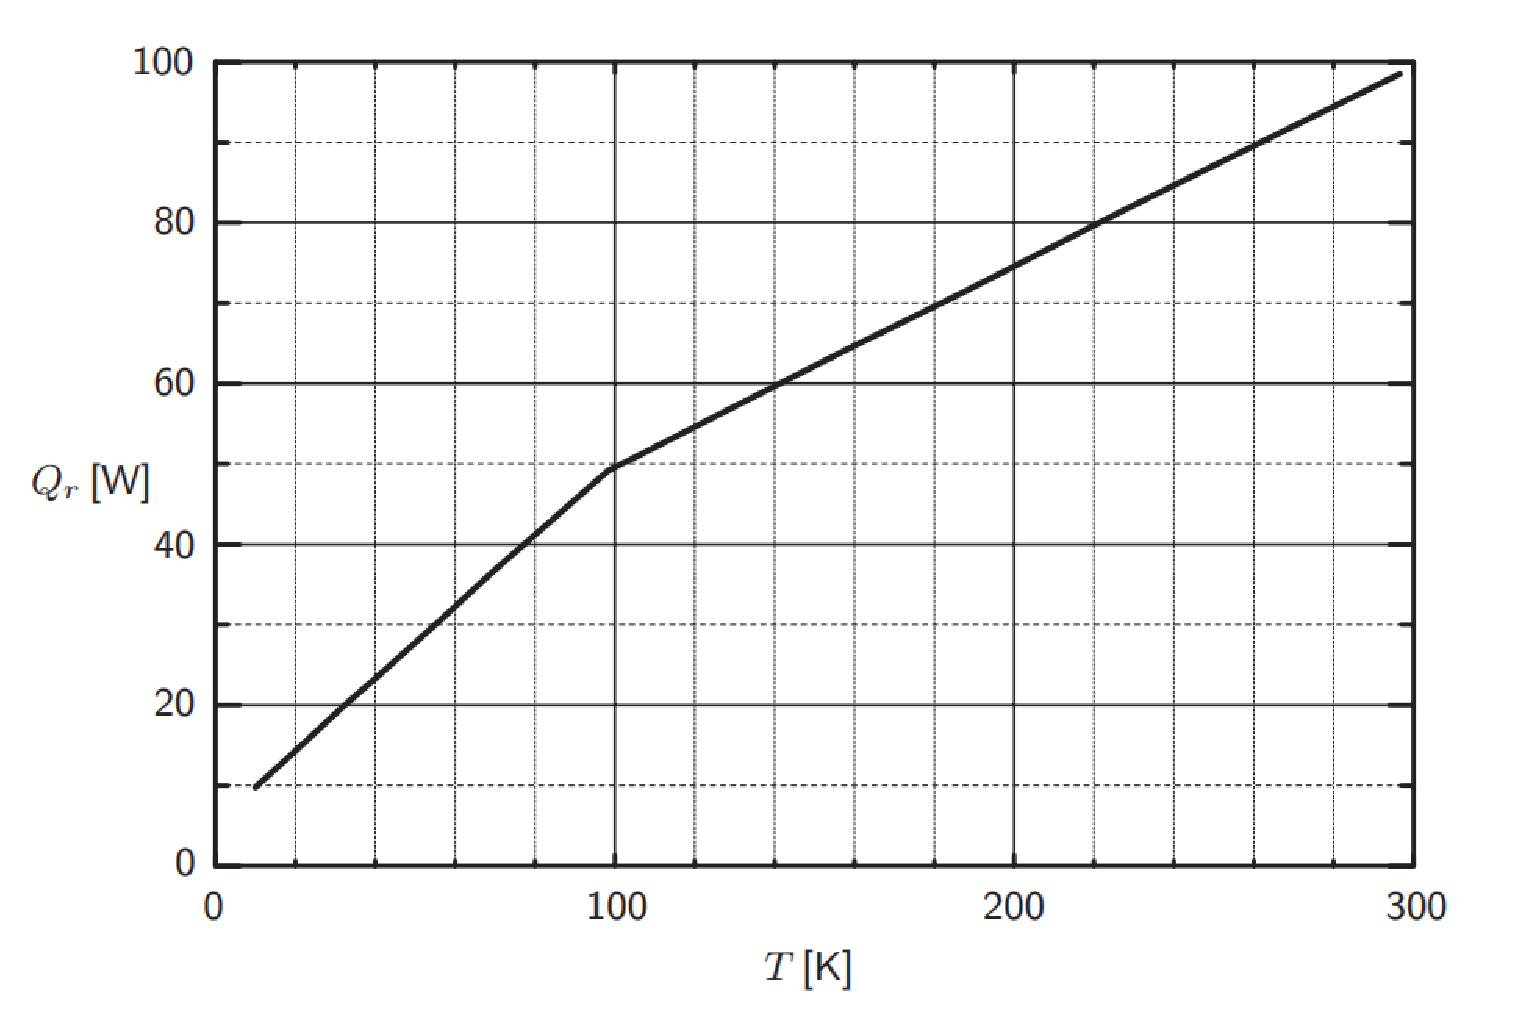
\includegraphics[scale=0.5]{chpt4/figs/fig4.7.eps}
	\caption{磁体制冷机的$Q_r(T)$曲线。}
\end{figure}
	
\colorbox{red}{表4.4}

表4.4列出了$Q_r(T)$,$C_{cu}(T)$和$\kappa(T)\equiv C_{cu}(T)/Q_{r}(T)$在给定温度下的值。
我们可以通过积分方程4.4,在特定的$T_i,T_{op},Q_r(T),M_{cu}$组合下解出$\tau_{cu}$:	
\begin{subequations}% 4.5
\begin{align}
\tau_{cn}&=\frac{M_{cu}}{\varrho_{cu}}\int_{T_{op}}^{T_i}\frac{C_{cu}(T)}{Q_r(T)}dT=\frac{M_{cu}}{\varrho_{cu}}\int_{T_{op}}^{T_i}\kappa(T)dT\\
M_{cu}&=\frac{\varrho_{cu}\tau_{cn}}{\int_{T_{op}}^{T_i}\kappa(T)dT}
\end{align}
\end{subequations}

在一些应用中,$\tau_{cu}$是主要的设计要求。可以看出,方程4.5b限制了在$\tau_{cu}$内可以冷却下来的铜的质量$\~{M}_{cu}$(这里代表磁体质量)。
对于给定的$T_i$和$T_o$组合,$\~{M}_{cu}$正比于$\tau_{cu}$。
表4.5给出了以图4.7中给出的$Q_r(T)$为基准的$T_i$,$T_o$和$\tau_{cu}$组合下的$\~{M}_{cu}$。
这样,如果磁体经4个小时从300 K冷却至30 K,受限的冷却质量是11.6 kg。

表4.5给出的结果清晰的指出了对于给定的$\tau_{cu}$,如果我们首先将磁体冷却至77 K,将可以极大的增加$\~{M}_{cu}$。
表4.3可以用于估计实现这个过程的所需LN2量。

\colorbox{red}{表4.5}


\subsection{讨论4.4:超流}
图4.8是常规氦($He^4$)的相图,其中给出了两种流体形式He I和He II[4.20]。
因为He II有独特的超高热导($k$)和超低黏性($\nu$)的独特性质,它被称为超流氦。
我们从相图中可以看出,沸点为4.22 K的常规氦 (He I)通过简单的加压即可变为He II。
当达到饱和压力5 kPa (37.8 torr)后,液体在2.18 K称为超流。
2.18 K被称为$\lambda$点,记为$T_\lambda$。
根据二流体模型,超流的比分在$T_\lambda$时为零,而随温度降低单调增加。
通过对比He II和常见物质的物性,我们可以看到超流氦的热导和黏性的独特性(表4.6)。

\textbf{传输性质}

因为超流氦的超高热导率,它常被用作超导磁体的制冷工质,通常运行于$\sim 1.8\ \mathrm{K}(<T_\lambda)$。
(尽管我们这里使用热导率的经典定义,即热导$\propto$温差。
在He II中,温差越小,等效热导率越大。等效热导率同样依赖于热通量。)
He II的搞热导率不允许液体中存在足以引起汽化的温度梯度。
这样,不像运行于4.2 K的He I冷却的磁体绕组,1.8 K的He II冷却的“无气泡”绕组不需要通道。
不过,这并不意味着He II可以在窄通道内无限制的传输热流。
类比于超导体中的临界电流,He II有一个临界热流密度。

\begin{figure}[htbp]
	\centering
	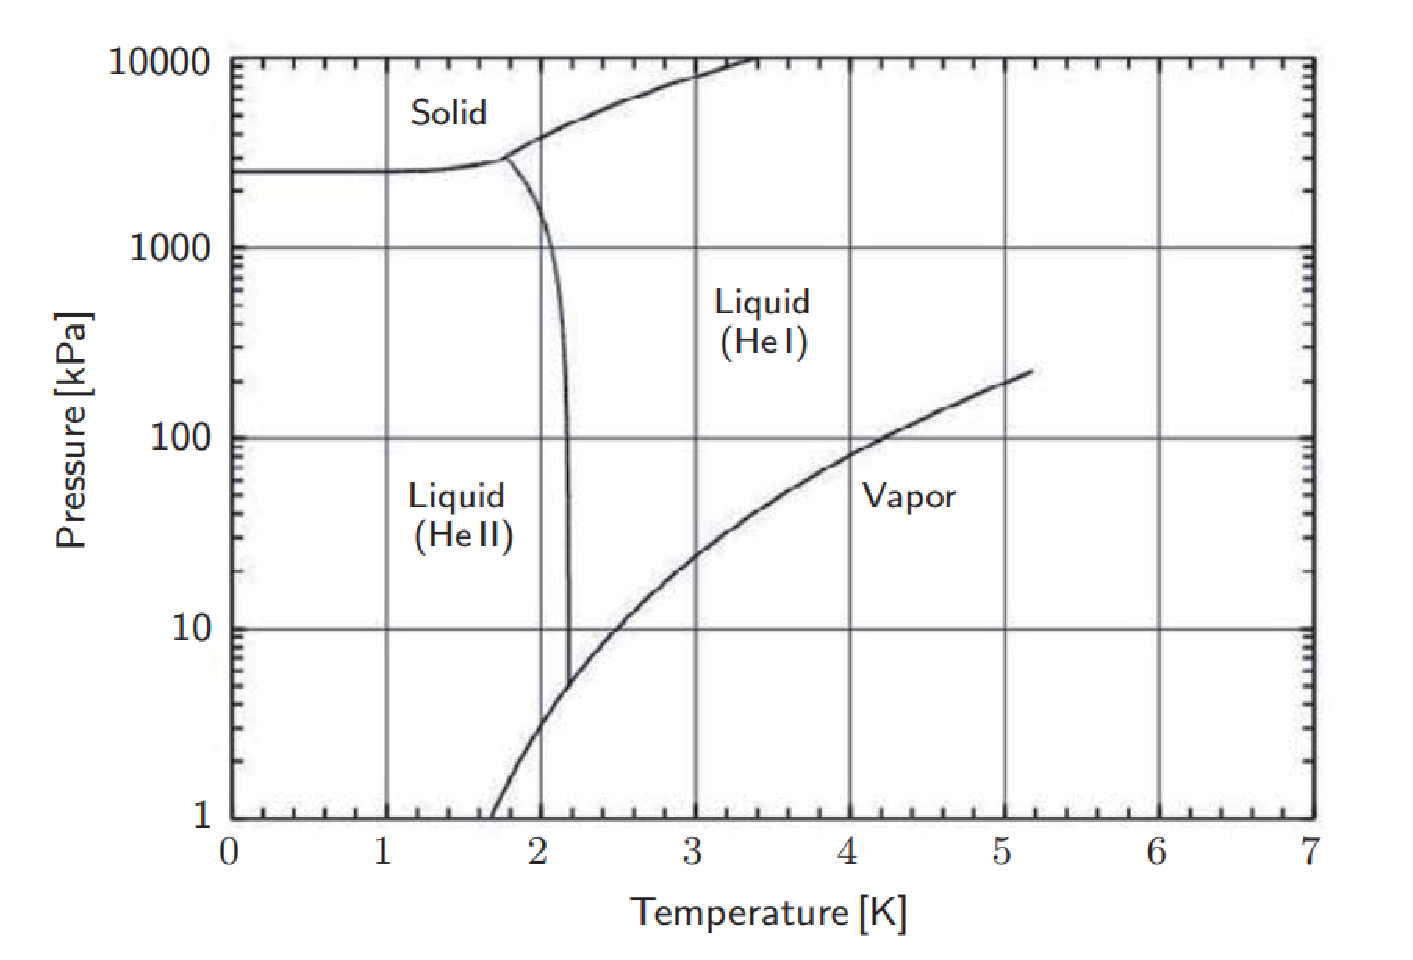
\includegraphics[scale=0.5]{chpt4/figs/fig4.8.eps}
	\caption{常规氦($He^4$)的相图。}
\end{figure}

\colorbox{red}{表4.6}

Bon Mardion、Claudet和Seyfert研究了He II通过窄通道的热流密度[4.21]。
图4.9以参数$X(T)$的形式给出了他们的结果:
\begin{equation}% 4.6a
X(T_{cl})-X(T_{wm})=q^{3.4}L
\end{equation}

式中,$T_{cl}$[K]是冷端温度,$T_{wm}$[K]是热端温度。$q[\mathrm{W/cm^2}]$是通过跨上述冷热两端
通道L [cm]的热流密度。方程4.6可用于通道自身不存在向液氮的额外热量输入的情况。
正常运行时,$T_{cl} = T_b$,其中$T_{b}$是容器温度;$T_{wm}$是绕组内部紧邻发热区域的液体问题,
不允许超过$T_\lambda$。当$T_{wm}=T_\lambda$时,从图4.9可以看出,$X(T_{wm})=0$,我们可将4.6简化为:
\begin{equation*}% 4.6b
X(T_b)=q_{c}^{3.4}L \tag{4.6b}
\end{equation*}

\begin{figure}[htbp]
	\centering
	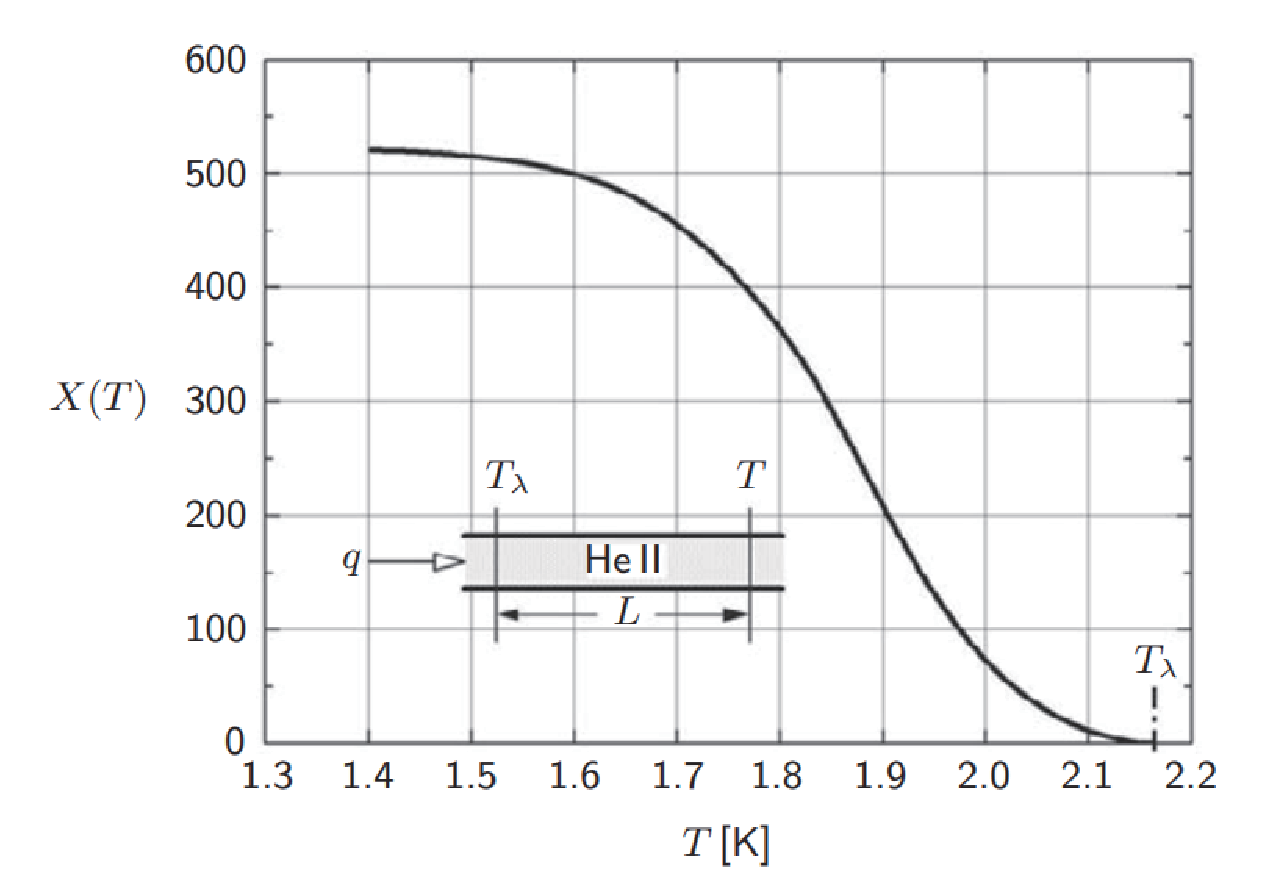
\includegraphics[scale=0.5]{chpt4/figs/fig4.9.eps}
	\caption{Bon Mardion、Claudet和Seyfert的研究结果。}
\end{figure}

对于$T_{wm} > T_\lambda$,从发热区域表面流出的热流被$q_{pk}$限定。
如图4.2所示,He I对应的值$\sim 1 \mathrm{W/cm^2}$。
方程4.6b指出,如果$T_b<2\ \mathrm{K}$,在磁体的尺度小于1 m时,极限将超过$1 \mathrm{W/cm^2}$。
在设计通道配置和尺度时,我们必须确保运行热流密度$q_{op}$不能超过方程4.6b给出的$q_c$。

\textbf{受热的通道}

当热量在通道的整个长度L上是均匀的而不是像上文讨论的仅在热端的时候,方程4.6b改为:
\begin{equation*}% 4.6c
X(T_b)=\frac{q_{c}^{3.4}}{4.4}L \tag{4.6c}
\end{equation*}

\textbf{B. 热传递——Kapitza热阻}

金属或其他热导材料与He II之间的热传递收到Kapitza热阻的限制。表面温度为$T_{cd}$[K]和处于温度为$T_b$[K]
之间的热传递通量$q_k[\mathrm{W/cm^2}]$为:
\begin{equation}% 4.7
q_k=a_k(T_{cd}^{nk}-T_{b}^{nk})
\end{equation}

表4.7给出了$a_k$和$n_k$的典型值。

\textcolor{red}{表4.7}



\subsection{讨论4.5:1.8 K过冷低温容器}
这里我们讨论一个浸泡于1 atm和1.8 K过冷潮流氦的超导磁体的低温容器。
随着运行温度从4.2 K降到1.8 K,磁体的性能显著提高,特别是浸泡冷却的NbTi磁体[4.25],因为
它在以下方面都有了显著提高:1)临界电流密度;2)导体和制冷剂之间的传热。

图4.10给出了用于混合III磁体系统的过冷1.8 K低温容器的示意图[4.26]。
位于容器外部的泵驱动液氦以质量流量$\.{m}_h$流动,这是由位于磁体腔内的1.8 K蒸发器决定的。
1.8 K/1 atm磁体腔通过管路连接至4.2 K/1 atm热源,热源位于窄通道上,一方面维持磁体腔在1 atm(过冷),
另一个方面降低从热源到磁体腔的液氦传导热输入。
电流引线穿过4.2 K热源,进入磁体腔,为两个液体腔提供电流连接。诸如支撑件等非直接与制冷循环有关的组件未在图中画出。
\begin{figure}[htbp]
	\centering
	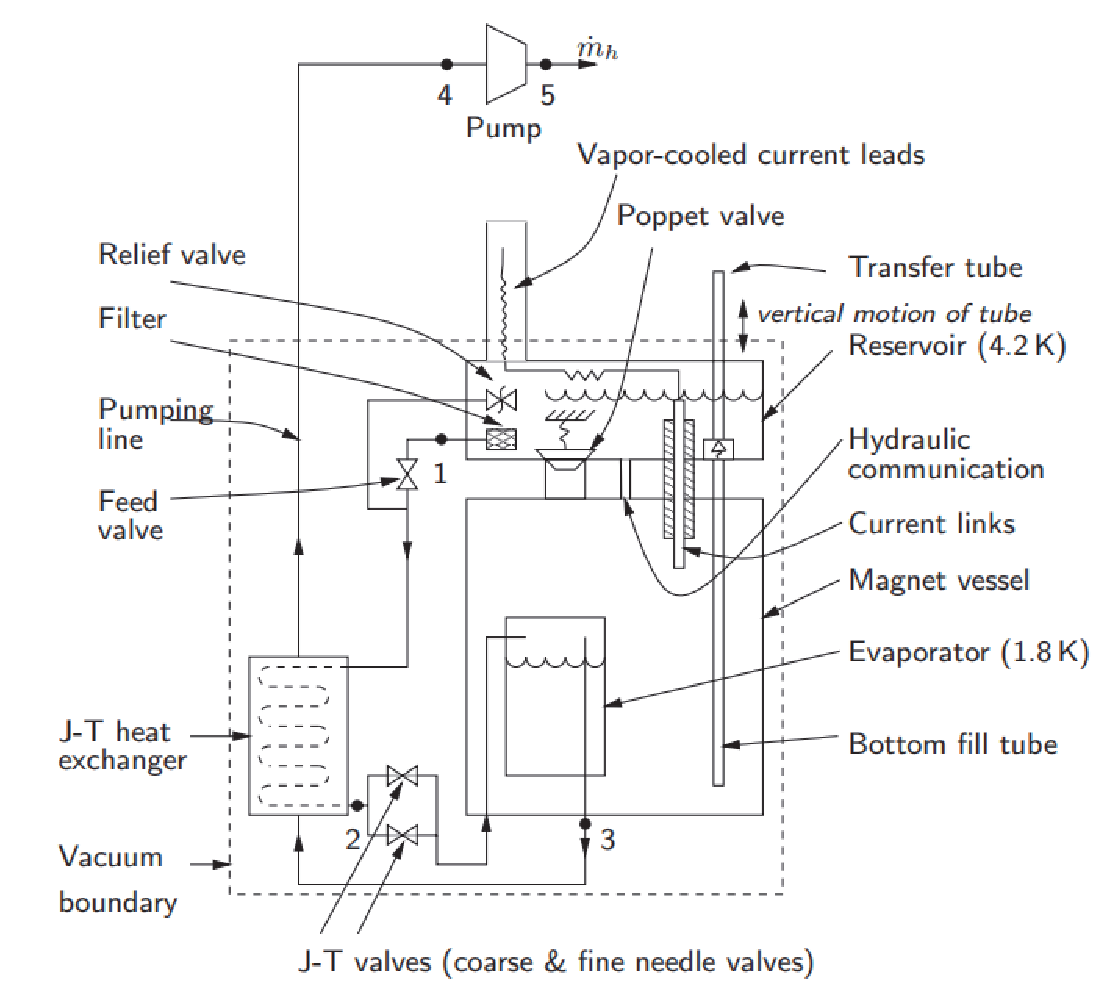
\includegraphics[scale=0.6]{chpt4/figs/fig4.10.eps}
	\caption{1.8 K过冷低温容器结构示意。}
\end{figure}

热源外部的点1透入的4.2 K/1 atm(760 torr)液氦是由J-T热交换器冷却后流过J-T阀的。
该阀将液氦等焓的从760 rorr减压至12.3 torr——J-T过程的更多问题,将在讨论4.6涉及——形成1.8 K/12.3 torr的气液混合物。
1.8 K液体进入汽化器,将磁体腔内的1 atm液体冷却,就像瓶子里的水被冰块冷却一样。
在它的回路上,1.8 K气体离开蒸发器,冷却J-T热交换器中流过来的4.2 K液体。

离开泵的时候,氦气得以纯化,而后存储在压力容器中。
从4.2 K热源排出的氦气通过气冷电流引线,也被存储于容器中。
来自容器的氦被液化然后转移至500 L存储杜瓦,在这里再不断的传输至4.2 K冷源以维持冷源的液位。
所以,该1.8 K低温容器是一个封闭系统。

在正常运行条件下,汽化器内的1.8 K/12.3 torr超流氦保持近乎不变的液位。
磁体腔的总的热负荷$Q_{1.8}$因此由汽化器产生的制冷量匹配。
$Q_{1.8}$从腔体通过汽化器壁面进入汽化器。

\textbf{1.8 K的制冷功率}

由汽化器提供的1.8 K的制冷功率,$Q_{1.8}$,可从应用于包围汽化器的控制体(c.v.)的热力学第一定律导出,如图4.11所示。
图中,$\.{m}_h$是进出控制体的质量流量。在稳态条件下,总的热输入$Q_{in}$和总的热输出$Q_{out}$之差即为
$Q_{1.8}$:
\begin{equation}% 4.8
Q_{out}-Q_{in}=Q_{1.8}
\end{equation}

\begin{figure}[htbp]
	\centering
	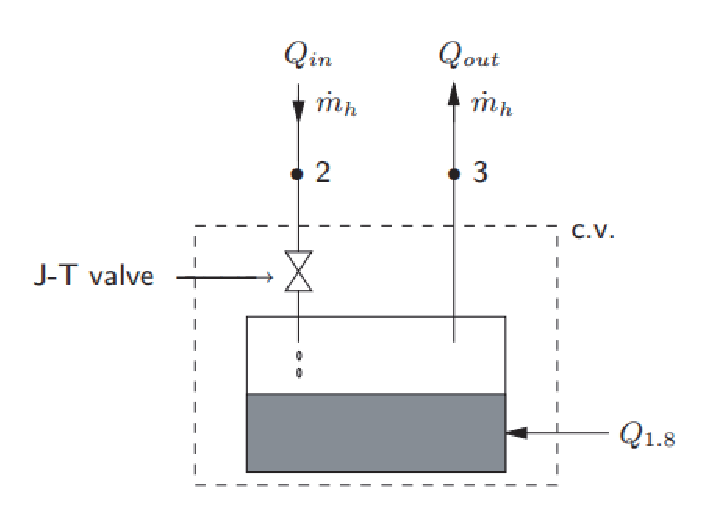
\includegraphics[scale=0.6]{chpt4/figs/fig4.11.eps}
	\caption{汽化器的热平衡。点2和点3在低温容器的位置见图4.10。}
\end{figure}

注意到,$Q_{1.8}$还等于汽化器的制冷负荷。$Q_{1.8}$主要由以下组成:
\begin{itemize}
	\item 磁体内的耗散——接头损耗和磁场变化时的交流损耗;这些损耗将在第七章讨论。
	\item 向磁体腔的热输入——传导:通过支撑结构和工作于4.2 K热源和1.8 K腔体之间的电流引线;
	超流通过压力变换通道热传导;腔体表面的热辐射和残余气体对流。
\end{itemize}

控制体的热输出,$Q_{out}$,可由$Q_{out}=\.{m}_h h_3$给出,式中,$h_3$是氦(气)在点3的焓。
类似的,$Q_{in}=\.{m}_h h_2$,式中$h_2$是氦(液)在点2的焓。解方程4.8,有:
\begin{equation}% 4.9
Q_{1.8}=\dot{m}_h(h_3-h_2)
\end{equation}

点1处于4.2 K,点3处于1.8 K。为了在给定流量下最大化$Q_{1.8}$,方程4.9中的$(h_3-h_2)$必须最大化:
点2的氦温度必须尽量接近1.8 K。
J-T热交换器将流入的4.2 K/760 torr液氦冷却为1.8 K/12.3 torr气氦。

\textbf{实例}\qquad 用下列参数确定$\.{m}_h$[g/s]以令$Q_{1.8}=20\ \mathrm{W}$:$P_2$ = 1 atm; $T_2$ = 3.0 K; $P_3$ = 12.3 torr,$T_3$ = 1.8 K。查附录II,我们有$h_3$(1.8 K, 12.3 torr; vapor)=24.02 J/g,$h_2$(3.0 K, 1 atm; liquid)=5.64 J/g,于是: 
\begin{equation*}% 4.9
Q_{1.8}=\dot{m}_h(24.02\ \mathrm{J/g}-5.64\ \mathrm{J/g})=20\ \mathrm{W}
\end{equation*}

解出上面的方程,我们得$\.{m}_h$=1.09 g/s,这相当于液氦的供应流量为31 L/s(4.2 K, 1 atm)。
除了这31 L/s的液氮供应,将液氦供应到热源以移除电流引线和其他热负荷也是必要的。

\textbf{B. 制冷泵功率需求}

假设泵过程是等焓、氦气是理想气体,我们可以计算足以将氦以$\.{m}_h$=1 g/s的流量从点4(12.3 torr/300 K)泵到点5(760 torr)的最小输入功。
对一个等焓泵,需要的泵功率为:
\begin{equation}% 4.10
P_s=Q_{1.8}=\dot{m}_h(\frac{\gamma}{\gamma-1})(P_4\nu_4)[(\frac{P_5}{P_4})^{\frac{\gamma-1}{\gamma}}-1]
\end{equation}

式中,理想气体的$\gamma=C_p/C_v$是5/3;$v_4$是点4的比体积,对300 K/12.3 torr的氦,该值为371$\mathrm{m^3/kg}$。带入$P_4=12.3\ \mathrm{torr}=1.64\times 10^3\ \mathrm{Pa}, P_5/P_4=61.8,\.{m}_h=0.001\ \mathrm{kg/s}$,我们得到$P_s=6400\ \mathrm{W}$。
注意到这是按理想气体得到的;实际的泵功率大约是20 kW。

\textbf{管线压降}\qquad 将点3(运行压力点)和点4之间的压降保持在12.3 torr以下是很重要的。
$P_4$越低——小于12.3 torr以保持$P_3=12.3$ torr——对$P_s$的要求越高。
就混合磁体III系统而言低温容器外的泵系统包一条内径15 cm,长13 m,有5个$90^\circ$弯,1个开闭阀的管路。它最大流速可达$\sim 2\ \mathrm{g/s}$,对应总压降小于1 torr。

同时,需要注意不要将污染物引入到汽化器。污染杂物可能会在最狭窄的区域——比如J-T阀——冻结,堵住管路。
在混合磁体III中,每一个J-T阀都有一个加热器以融化冻结的污物。

\textbf{C. 液压交换通道的漏热}

对混合磁体III的低温容器,用以保持磁体腔内压1 atm的液压交换通道有效截面为$2.6\ \mathrm{mm^2}$。
它的连接热源的氦和磁体腔的有效长度L是10 cm。使用图4.9中给出的Bon
Mardion-Claudet-Seyfert图,假设氦在热源下部的温度为$T_\lambda$,在磁体腔的温度为1.8 K。我们可以计算这个通道内的超流氦从4.2 K热源传入1.8 K磁体腔的热输入。

正如4.4A论及的,对于一个充满1 atm超流氦的狭窄通道,我们可以使用方程4.6。其中涉及通道长度$L[\mathrm{cm}]$和对应两个末端温度的$X(T)$——热端$T_{wm}$和冷端$T_{cl}$,相应的传导热$q\ \mathrm{W/cm^2}$。
现有$T_{wm}=T_\lambda, T_{cl}=1.8,L=10$,以及从图4.9读出的$X(T_\lambda)=0,X(1.8)=360$。
将上述值带入4.6,我们有$q=2.87\ \mathrm{W/cm^2}$。通道的截面积是$2.6\ \mathrm{mm^2}$,那么通过液压通道进入到1.8 K磁体腔的总传导热输入为$\sim 75\ \mathrm{mW}$。

热源的底部区域放置碳电阻以测量该区域的液体温度。尽管测量表明这个特定热源底部的液体温度是$\sim 3\ \mathrm{K}$(此类1.8 K低温容器的典型值),但热源底部的液体应该非常接近$T_\lambda$。
因为$2.6\ \mathrm{mm^2}$在磁体失超时对限制1.8 K磁体腔的过压不够,低温容器还设置一个$40\ \mathrm{mm^2}$的提升阀。正常运行时,提升阀由弹簧控制常闭;磁体腔内压力过高时,阀打开。

\textbf{D. 4.2 K液体补液}

混合磁体III的冷却模式的最后步骤之一是将磁体腔内的液氦从4.2 K冷至1.8 K。
冷量由汽化器提供,汽化器内源源不断的充入液氦,液氦从最初热源中的4.2 K经J-T换热器冷却后进入汽化器,而后泵走。
对一个250 L的磁体腔的需液量,我们可以估算出液氦从4.2 K冷至1.8 K磁体腔所需的补液量。

液体密度在1 atm、4.2 K和1.8 K时分别为$125\ \mathrm{kg/m^3}$和$147\ \mathrm{kg/m^3}$。
这样,对混合III,250L的腔体开始需要大约31 kg的4.2 K液氦,最终需要大约37 kg的1.8 K液氦。
也就是说,必须向腔体补充大约6 kg的液氦。以4.2 K的体积计。相当于大约50 L。 

尽管交换通道$2.6\ \mathrm{mm^2}$的截面足以提供在2小时冷却时间传输上述额外质量液体,
总流体截面$40\ \mathrm{mm^2}$的提升阀在此过程保持开启,直到腔内液体温度达到$T_\lambda$。

\textbf{E. 4.2 K热源和1.8 K腔体之间的电流引线}

电流引线必须从热源底部连接到1.8 K腔体内磁体的端部。
习惯上常采用复合超导体做电流引线。
在这个应用中,常规金属(铜)的截面占比必须足够小,以减小金属从热源到腔体的热传导;同时又要足够大以稳定复合超导体。
“干式”引线标准(讨论4.15)于此应,因为引线两端在混合III低温容器内本质上是隔离的,
分隔热源和1.8 K腔的垂直间隙处于真空中。

我们可以证明,载流为$I_t$的正常态引线稳态温度峰值出现在引线的热源端。
通过选择引线复合超导体的电流分布温度($T_{cs}$)远大于热源底部液氦温度$T_\lambda$,
我们可以确保电流引线的稳定运行(第六章讨论 $T_{cs}$)。

正常态引线的稳态温度特性的表达式可以从方程4.52得到(讨论4.15):
\begin{equation}% 4.11
T(z)=-\frac{\tilde{\rho}I_{t}^{2}}{2A^2\tilde{k}}z^2+[\frac{(T_\ell-T_0)}{\ell}+\frac{\tilde{p}I_{t}^2\ell}{2A^2\tilde{k}}]z+T_0
\end{equation}

方程4.11中,复合超导体的$z=0$处于1.8 K腔内,$z=\ell$在热源内。
$\tilde{\rho}$和$\title{k}$分别是复合常规金属的电阻率和热导率。
$A$和$\ell$分别是引线的截面积和冷端$T_0$(1.8 K)、热端$T_\lambda$($\simeq T_\lambda$)间的长度。
根据讨论4.15,额定载流$I_t=I_0$的干式引线满足以下关系:
\begin{equation}% 4.12
(\frac{I_0\ell}{A})_{dr}=\sqrt{\frac{2\tilde{k}(T_\ell-T_0)}{\dot{\rho}}}
\end{equation}

联立上面两个方程,定义一个新的变量$\xi\equiv z/\ell$,有:
\begin{equation}% 4.13
T(\xi)=-(T_\ell-T_0)\xi^2+2(T_\ell-T_0)\xi+T_0
\end{equation}

$\xi=1$时,$dT/d\xi=0$,对应最高温度。
因为这个位置是在$\xi=1$处,也即最高温度是$T_\ell\simeq T_\lambda$。
换句话说,即使引线在超导态滑入正常态,如果引线满足方程4.12给出的标准,那么传导冷却仍足以限制最高温度到$T_\lambda$,不会超过引线的热端温度。


\subsection{讨论4.6:J-T过程}
焦耳-汤姆森(J-T)过程,是指气体通过受限通道,即J-T阀,而降低压力并改变温度的过程,该过程是不做功的绝热膨胀(等焓)。这个过程是正、负或是零,取决于气体性质、起始温度和始末压力。对于初始压力为10 atm,终了压力为1 atm的氦,如果初始温度小于$\sim 7.5\ \mathrm{K}$,就能被液化。因为过程不可逆,J-T过程液化的结果总是比等熵膨胀产生的液化量要少。例如,初始温度为6 K,压力为10 atm——液化器的典型值——下面的等焓关系可以用来计算4.2 K和1 atm下可液化的氦量。
\begin{equation}% 4.14
h_g(6\ \mathrm{K},10\ \mathrm{atm})=x_\ell h_\ell(4.2\ \mathrm{K},1\ \mathrm{atm})+(1-x_\ell)h_g(4.2\ \mathrm{K},1\ \mathrm{atm})
\end{equation}

从4.14,我们得到$x_\ell=0.47$。如果同样的气体等熵膨胀,类似于方程4.14焓关系的熵关系给出的数值是$x_\ell=0.85$。尽管液体产生效率低,但J-T膨胀以其结构的简单性,被用于很多氦液化器的最后阶段。


\subsection{问题4.2:基于制冷机的小型氦液化器}
如本章开始提到的,随着制冷机的大规模使用,多数的直流超导磁体,无论是LTS还是HTS,都将
可能采用由制冷机冷却的“干式”(无制冷剂)运行方式。
多数的制冷剂冷却的磁体,其制冷机/磁体组合体是安装于同一低温容器内的。而对于一些应用,
磁体和制冷机分别装在不同的低温容器中。
图4.12给出了一个这样的系统的示意图,它是慢“神奇角自旋(MAS)”NMR磁体。
在这样一个磁体中,主磁场与磁体角度为54.73$\circ$(问题2.5),磁体绕轴旋转。
如图4.12可见,磁体的主要冷源可以由安装在距离磁体大约1 m的静态制冷机提供。 
系统中的标示数字的组件,在图注中都给出了名称。

简单来说,系统容许磁体/低温容器组合体(图4.12中的组件2)旋转,液氦流源源不断的以流量$\.{m}_h$
由小型液氦液化器中经旋转轴输送到磁体低温容器内。小型液化器的初级冷源来自第二低温容器(14)内的制冷机。
基于制冷机的小型液化器的热力学过程是本问题的核心。
\begin{figure}[htbp]
	\centering
	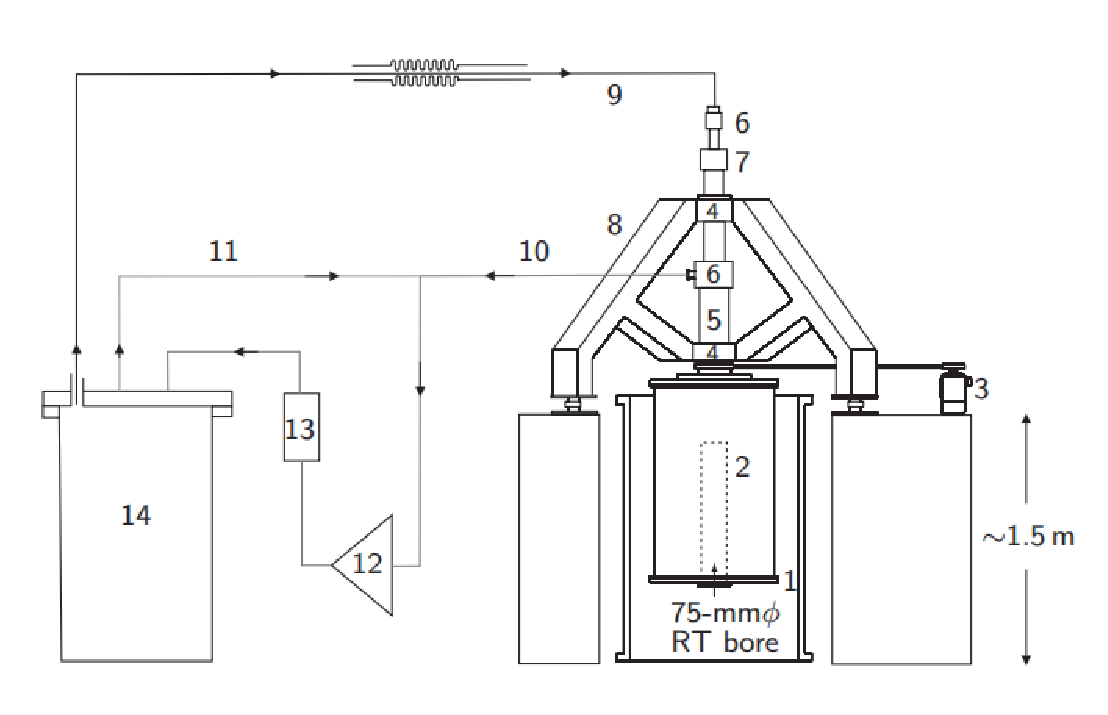
\includegraphics[scale=0.7]{chpt4/figs/fig4.12.eps}
	\caption{配合一个基于制冷机的小型氦液化器的超导磁体系统示意图,它应用于慢MAS NMR系统。其中,
	运行于持续模式的超导磁体由来自基于制冷机的小型液化器的液氦冷却,
	产生一个与旋转轴为$54.73\circ$的磁场。1:地磁补偿线圈(静止);2:磁体/低温容器组合体;3:驱动电机;
4:轴承;5:旋转轴;6:旋转关节;7:滑环;8:支撑三脚架;9:液氦输运管;10:氦恢复管;11:热氦回流管;
12:压缩器;13:冷阱;14:基于制冷机的小型液化器。}
\end{figure}

\begin{figure}[htbp]
	\centering
	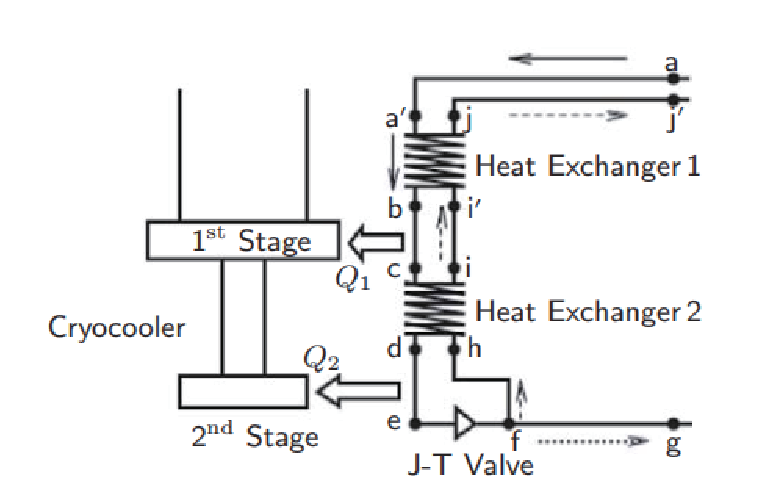
\includegraphics[scale=0.7]{chpt4/figs/fig4.13.eps}
	\caption{基于制冷机的小型氦液化器示意图。}
\end{figure}

图4.13给出了小型液化器的细节。它由热-冷流(质量流量$\.{m}_{he}$,压力10 atm)和冷-热氦气流($\.{m}_v$,1 atm)
和作为冷源的制冷机的一二级冷头组成。
整个过程假设为理想的,也就是无压降;两个流之间是无温差的理想热交换。

\textbf{热-冷氦流}——图4.13中的实箭头

点$a$:小型液化器的入口,来自冷阱(图4.12中的13):$T_a=295\ \mathrm{K}; P_a=10\ \mathrm{atm}$。

点$a^\prime$:热交换器1的入口:热力学等同于点a。

点$b$:热交换器1的出口(一级冷头入口):$T_b$。

点$c$:热交换器2的入口(一级冷头出口):$T_c$。点b和点c之间,一级冷头从氦流中带走热量$Q_1$。

点$d$:热交换器2的出口(二级冷头入口):$T_d$。

点$e$:二级冷头出口(J-T阀入口):$T_e$。点d和点e之间,二级冷头从氦流中带走热量$Q_2$。

点$f$:J-T阀出口:$T_f=4.22\ \mathrm{K};P_f=1\ \mathrm{atm};\.{m}_v;\.{m}_{\ell p}$(液化质量流量)。
LHe到点g,由点箭头标识。

\textbf{冷-热氦流}——图4.13中的虚线箭头

点$g$:到LHe输运管(图4.12中的9):$T_g=4.22\ \mathrm{K};P_g=1\ \mathrm{atm};\.{m}_{\ell}$。

点$h$:热交换器2入口:$T_h=4.22\ \mathrm{K};P_h=1\ \mathrm{atm};\.{m}_v;\.{m}_{\ell r}=\.{m}_{\ell p}-\.{m}_{\ell}$(LHe回流质量流量)。

点$i$:热交换器2出口:$T_i=T_c;P_i=1\ \mathrm{atm}$。

点$i^\prime$:热交换器1入口:热力学上等同于点i。

点$j$:热交换器1出口:$T_j=295\ \mathrm{K};P_j=1\ \mathrm{atm}$。

点$j^\prime$:到热氦出管(图4.12中的10)。

a) 证明在J-T过程实现氦液化速率$\.{m}_{\ell p}\simeq0.202\ \mathrm{g/s}$和$\.{m}_{he}=1.0\ \mathrm{g/s}$,点e的温度$T_e=7\ \mathrm{K}(P_e=10\ \mathrm{atm})$。

b) 在$T_d$=8 K (和$P_d$ =10 atm)时,计算7 K时的制冷机二级冷头功率$Q_2$。注意应用$T_e=7\ \mathrm{K}(P_e=10\ \mathrm{atm})$。

c) 对一台有二级冷头的制冷机,4.22 K时它的$Q_2$是多少?

d) 在$T_b$ = 46 K和$T_c$ = 30 K ($P_b = P_c =$ 10 atm)时,计算30 K时一级冷头的制冷功率$Q_1$。

e) 假设热交换器2是理想的,即对环境无热损耗,热-冷流($\.{m}_{he}$=1.0 kg/s)和冷-热流($\.{m}_{v}$和$\.{m}_{\ell r}$)之间的热交换是完全的,证明
$\.{m}_{\ell r}$=0.158 g/s,从而$\.{m}_{\ell}$=0.044 g/s。假设$T_c=T_d$=30 K。

f) 类似的,证明两个流之间的热交换器1的完全热交换与$\.{m}_{\ell r}$=0.158 g/s一致。
假设$T_b$=46 K,$T_{i^\prime}$=30 K,$T_{a^\prime}=T_j$=295 K。

g) 应用方程4.10,计算压缩机(图4.12中的12)为了驱动$\.{m}_{he}$=1.0 kg/s的热氦流从$P_j$=1 atm到
$P_a$=10 atm所需的等熵功率。

\subsubsection{问题4.2之解}
a) 因为J-T过程焓不变,下面的焓等式关系保持:
\begin{equation*}% S2.1
h_{he}(7\ \mathrm{K},10\ \mathrm{atm})=x_\ell h_\ell(4.22\ \mathrm{K},1\ \mathrm{atm})+(1-x_\ell)h_v(4.22\ \mathrm{K},1\ \mathrm{atm}) \tag{S2.1}
\end{equation*}

式中,$h_{he}(7\ \mathrm{K},10\ \mathrm{atm})$=26.00 J/g,是氦在7 K和10 atm下的焓;
$x_\ell$是4.22 K和1 atm时的液体质量占比;$h_\ell(4.22\ \mathrm{K},1\ \mathrm{atm})$=9.71 J/g,
是液氦在4.22 K和1 atm时的焓;$h_v(4.22\ \mathrm{K},1\ \mathrm{atm})$=30.13 J/g,是气氦在4.22 K和1 atm
时的焓。解方程S2.1,我们有:
\begin{align*}% s2.2
x_\ell&=\frac{h_{he}(7\ \mathrm{K},10\ \mathrm{atm})-h_v(4.22\ \mathrm{K},1\ \mathrm{atm})}{h_\ell(4.22\ \mathrm{K},1\ \mathrm{atm})-h_v(4.22\ \mathrm{K},1\ \mathrm{atm})}\\ \notag
&=\frac{(26.00\ \mathrm{J/g}-30.13\ \mathrm{J/g})}{(9.71\ \mathrm{J/g}-30.13\ \mathrm{J/g})}=0.202  \tag{S2.2}
\end{align*}

在$\.{m}_{he}$=1.0 g/s时,有$x_\ell$=0.202,$\.{m}_{\ell p}$=0.202 g/s,$\.{m}_{v}$=0.798 g/s。

b) 在点d和点e之间应用下面的功率方程:
\begin{equation*}% S2.3
\dot{m}_{he}h_{he}(8\ \mathrm{K},10\ \mathrm{atm})=Q_2+\dot{e}_{he}h_{he}(7\ \mathrm{K},10\ \mathrm{atm})
\end{equation*}

从S2.3中解出$Q_2$,有:
\begin{align*}% s2.3
Q_2&=\dot{m}_{he}[h_{he}(8\ \mathrm{K},10\ \mathrm{atm})-h_{he}(7\ \mathrm{K},10\ \mathrm{atm})]\\\notag
&=(1\ \mathrm{g/s})(33.44\ \mathrm{J/g}-26.00\ \mathrm{J/g})=7.44\ \mathrm{W}
\end{align*}

c) 图4.6给出的二级冷头的性能数据表明该制冷机在4.2 K时的制冷容量1 W可已在7 K时提供4 W冷量。
于是,一台7 K时容量为7.44 W的制冷机大概在4.2 K可以提供2 W冷量。
4.22 K时具有冷量$\sim 2$ W的制冷机有望在2010年前后可以商业化。

d) 类似于S2.3的方程可以应用在点b和点c之间:
\begin{equation*}% 2.4
\dot{m}_{he}h_{he}(46\ \mathrm{K},10\ \mathrm{atm})=Q_1+\dot{m}_{he}h_{he}(30\ \mathrm{K},10\ \mathrm{atm})
\end{equation*}

从S2.4中,我们可以得到:
\begin{align*}% S2.4
Q_1&=\dot{m}[h_{he}(46\ \mathrm{K},10\ \mathrm{atm})-h_{he}(30\ \mathrm{K},10\ \mathrm{atm})]\\\notag
&=(1\ \mathrm{g/s})(252\ \mathrm{J/g}-168\ \mathrm{J/g})\simeq 84\ \mathrm{W}
\end{align*}

图4.6给出的性能数据表明,尽管一台制冷机在4.22 K时可以提高到2 W,也不能实现$Q_1\simeq 84$ W。
这时要求一台具有增强二级制冷功率的制冷机。

e) 从点$c$到点$d$的热-冷流的总焓减必须等于从点$h$到点$i$的冷-热流的总焓增:
\begin{align*}% S2.5
&\dot{m}[h_{he}(30\ \mathrm{K},10\ \mathrm{atm})-h_{he}(8\ \mathrm{K},10\ \mathrm{atm})]\\\notag
&=(\dot{m}_v+\dot{m}_{\ell r})h_v(30\ \mathrm{K},1\ \mathrm{atm})-[\dot{m}_vh_v(4.22\ \mathrm{K},1\ \mathrm{atm})+\dot{m}_{\ell r}h_l(4.22\ \mathrm{K},1\ \mathrm{atm})] \tag{S2.5}
\end{align*}

从S2.5中解出$\dot{m}_{\ell r}$:
\begin{align*}% page 246
\dot{m}_{\ell r}&=\frac{\{\dot{m}_{he}[h_{he}(30/10)-h_{he}(8/10)]-\dot{m}_v[h_v(30/1)-h_{v}(4.22/1)]\}}{h_v(30/1)-h_{l}(4.22/1)}\\\notag
&=\frac{(1\ \mathrm{g/s})(168.4\ \mathrm{J/g}-33.44\ \mathrm{J/g})-(0.798 \ \mathrm{g/s})(170.2J\ \mathrm{J/g}-30.13\ \mathrm{J/g})}{(170.2\ \mathrm{J/g}-9.71\ \mathrm{J/g})}\\\notag
&\simeq 0.144 \ \mathrm{g/s}
\end{align*}

因为$\dot{m}_{\ell}=\dot{m}_{\ell p}-\dot{m}_{\ell r}$,我们得到$\dot{m}_{\ell}\simeq 0.202-0.144=0.058\ \mathrm{g/s}$,这对应液体体积流量$\sim$ 1.7 L/h以及制冷功率1.2 W。

f) 从点$a^\prime$到点$b$的热-冷流热损耗等于从点$i^\prime$到点$j$的冷-热流热增:
\begin{align*}% S2.6
\dot{m}_{\ell r}[&h_{he}(295\ \mathrm{K},10\ \mathrm{atm})-h_{he}(46\ \mathrm{K},10\ \mathrm{atm})]\\\notag
&=(\dot{m}_v+\dot{m}_{\ell r})[h_v(295\ \mathrm{K},1\ \mathrm{atm})-h_{v}(30\ \mathrm{K},1\ \mathrm{atm})] \tag{S2.6}
\end{align*}

方程S2.6等式左侧:
\begin{align*}% S2.7a
\dot{m}_{he}[h_{he}(295\ \mathrm{K},10\ \mathrm{atm})&-h_{he}(46\ \mathrm{K},10\ \mathrm{atm})]\\\notag
&=(1\ \mathrm{g/s})(1550.0\ \mathrm{J/g}-253.9\ \mathrm{J/g})\\\notag
&\simeq 1296\ \mathrm{W} \tag{S2.7a}
\end{align*}

类似的,方程S2.6等号右侧:
\begin{align*}% 2.7b
(\dot{m}_v+\dot{m}_{\ell r})&[h_{he}(295\ \mathrm{K},1\ \mathrm{atm})-h_{he}(30\ \mathrm{K},1\ \mathrm{atm})]\\\notag
&\simeq(0.798\ \mathrm{g/s}+0.144\ \mathrm{g/s})(1547.0\ \mathrm{J/g}-170.2\ \mathrm{J/g})\\\notag
&\simeq 1297\ \mathrm{W/s} \tag{S2.7b}
\end{align*}

事实上,方程S2.7a和S2.7b是相等的,舍入误差在$\sim 0.1\%$以内。

g) 应用方程4.10,我们可以得到理想压缩功率:
\begin{equation*}% s2.8
P_s=\dot{m}_h\left(\frac{\gamma}{\gamma-1}\right)(P_jv_j)[\left(\frac{P_a}{P_j}\right)^{\frac{\gamma-1}{\gamma}}-1]\tag{S2.8}
\end{equation*}

式中,理想气体的$\gamma=C_p/C_v$是5/3;$v_i$是压缩机入口在$P_j$=1 atm时的比体积,对295 K的氦,
该值$\simeq 6\ \mathrm{m^3/kg}$。代入$P_j$=1 atm$\simeq 1\times 10^5$ Pa,$P_a/P_j$=10,$\.{m}_h$=0.001 kg/s,
我们得到$P_s$=2.3 kW(或3马力)。
上面的计算是针对理想气体的,实际的泵功率大概要到7 kW。

当然,实际的小型氦液化器中,由于热交换的“不完全”以及热-冷流和冷-热流的压降,产液量必然小于理想液化器情况:
$\.{m}_{\ell p}$以及$\.{m}_{\ell}$仅能达到理想情况的1/2。


\subsection{讨论4.7:制冷机 vs. 制冷回环器}
本节讨论两种干式磁体(无制冷剂)的冷源。

\textbf{制冷机}\qquad 当前,所有的干式(无制冷剂)磁体,不论LTS还是HTS,都是由制冷机制冷的。制冷机的冷头连接于
作为磁体一部分的低温恒温器的一端。图4.14给出了制冷机制冷干式磁体的示意图:
一级冷头连接于热辐射屏,二级冷头连接于磁体腔。对于大型的干式LTS磁体,满足LTS磁体的稳定性是个挑战,即满足
$\Delta T_{op}/T_{op}\simeq 0$。其中,$\Delta T_{op}$是最冷点(接近二级冷头)和最热点(据二级冷头最远处)的温差。
\begin{figure}[htbp]
	\centering
	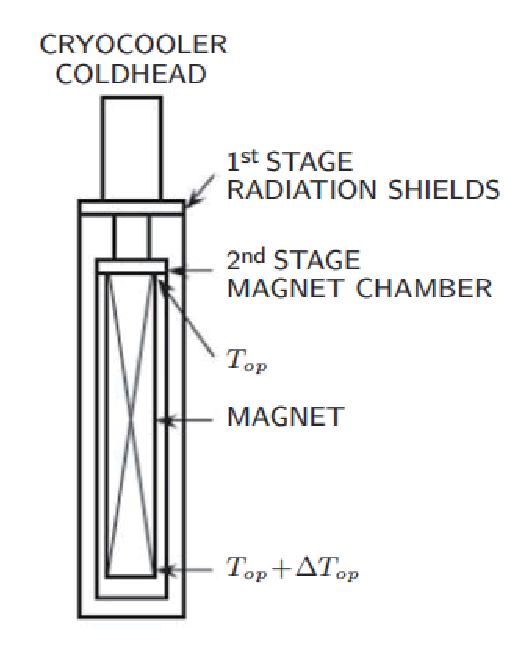
\includegraphics[scale=0.6]{chpt4/figs/fig4.14.eps}
	\caption{制冷机制冷的干式磁体示意图。}
\end{figure}

\textbf{制冷回环器}\qquad 为了保持磁体温度的均匀,即$\Delta T_{op}/T_{op}\simeq 0$,为制冷机配套制冷回环器
是有利于干式超导磁体的。如图4.15所示,制冷回环器是二级均配套了冷氦回环器的二级制冷机。
辐射屏壁面或磁体腔壁面装有冷却绕组,回环器迫使高压冷液氦通过上述绕组。
制冷回环器相比制冷机有两个优势:1) 它可实现对磁体腔体表面大部分区域的冷却,这样磁体不论大小,都可以满足$\Delta T_{op}/T_{op}\simeq 0$的条件。尽管对HTS磁体,$\Delta T_{op}$很容易超过1 K;2) 冷源和磁体恒温器通过柔性液氦管连接,
可以简单的解耦。

制冷回环器的一个早期应用是混合III磁体[3.14]。低温容器的辐射屏维持于其运行温度,一个回环器保持一组辐射屏为90 K,另一组
回环器保持另一组——用于1.8 K磁体恒温器的——在20 K。

\begin{figure}[htbp]
	\centering
	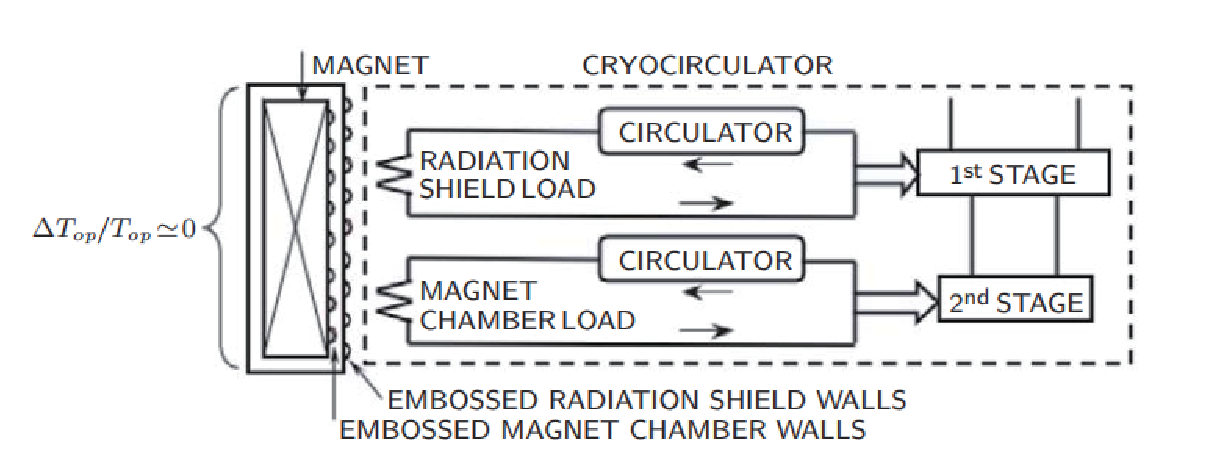
\includegraphics[scale=0.6]{chpt4/figs/fig4.15.eps}
	\caption{制冷回环器冷却磁体示意图。}
\end{figure}



\subsection{讨论4.8:辐射传热}
本节我们以混合III磁体为例,讨论由辐射传入恒温容器内的热。辐射传热的理论基础是Stefan-Boltzmann方程:
\begin{equation}% 4.15
q_r=\epsilon_r\sigma T^4
\end{equation}

式中,$q_r$是温度为$T$[K]的表面的辐射热流$[\mathrm{W/m^2}]$。$\epsilon_r$是$T$下的总发射系数。
$\sigma$是Stefan-Boltzmann常数,$5.67\times 10^{-8}\ \mathrm{W/m^2 K^4}$。
实际计算低温容器的辐射热输入并不像上式给出的这样直接,主要是确定辐射热量的两个表面的$\epsilon_r$准确值很难。
对于发射系数分别为$\epsilon_{cl}$和$\epsilon_{wm}$的平行板,一板处于低温$T_{cl}$,一板处于高温$T_{wm}$,
有效总发射系数可由下式给出:
\begin{equation}% 4.16
\epsilon_r=\frac{\epsilon_{cl}\epsilon_{wm}}{\epsilon_{cl}+\epsilon_{wm}-\epsilon_{cl}\epsilon_{wm}}
\end{equation}

尽管理论上区分平行板、圆柱、球等配置方式,但多数低温容器中,平行板公式可用于上述三种配置
(非平行配置通常是有不等面积的表面)。
这是因为:1) 多数低温容器中,分隔两个板的军力通常远小于表面的尺度;2) 由这种几何近似引起的热辐射计算误差远小于
表面发射系数计算的不确定性误差。于是,方程4.15修正为:
\begin{equation}% 4.17
q_r=\epsilon_r\sigma(T_{wm}^4-T_{cl}^4)
\end{equation}

表4.8给出了一些材料在两种特定温度下的$\epsilon_r$和$q_r$典型值。

\textbf{实例}\qquad 这里我们首先计算混合III的4.2 K磁体腔接收的来自20 K和80 K屏的总热输入。
磁体腔表面均为机械抛光的不锈钢,面积为:1) 面向20 K辐射屏为7.3 $\mathrm{m^2}$;2)面向80 K辐射屏为2.8 $\mathrm{m^2}$。
为了简化计算,我们使用方程4.17的平行板模型,并且认为冷热面积相同。
使用表4.8给出的机械抛光不锈钢表面$q_r$近似值,有:
\begin{align*}
\mbox{20 K板对腔体:} &Q_r\simeq (0.4\times 10^{-3}\ \mathrm{W/m^2})(7.3\ \mathrm{m^2})\simeq 3\ \mathrm{mW}\\
\mbox{80 K板对腔体:} &Q_r\simeq (162\times 10^{-3}\ \mathrm{W/m^2})(2.8\ \mathrm{m^2})\simeq 3\ \mathrm{mW}
\end{align*}

\textcolor{red}{表4.8}

我们还可以计算对着300 K表面的80 K辐射屏的热输入;对着300 K表面的80 K板的总面积是$11.7\ \mathrm{m^2}$。
同样,我们假设平行板的形状相同,即对着80 K板的300 K板的总面积也是$11.7\ \mathrm{m^2}$。

使用表4.8中机械抛光不锈钢表面的合适$q_r$值,我们有:
\begin{align*}
\mbox{300 K板对80 K板:} &Q_r\simeq (55\ \mathrm{W/m^2})(11.7\ \mathrm{m^2})=644\ \mathrm{W}
\end{align*}

\textbf{A. 超级绝热层的效果}

可以从表4.8看出,传入低温容器最大的辐射热负荷是来自80 K屏,它从300 K表面接收热量。
于是,习惯上在80 K和300 K表面间的真空空间($<10^{-4}$torr)之间放置一定数量的0.5$\mu $m的铝膜Mylar片——即超级绝热。
加入$N_i$层超级绝热后,方程4.17修改为:
\begin{equation}% 4.18
q_r=\frac{\epsilon_r}{N_i+1}\sigma(T_{wm}^4-T_{cl}^4)
\end{equation}

方程4.18表明,一层超级绝热就可以将$q_r$降低两个量级。通常的规则是在1 cm间隙使用大约10-20层。
同时,为了最小化固体导热路径,超级绝热层要么本身起皱的,要么就要在两层之间垫间隔物(表4.8最后三行给出的
是在三个温区内超级绝热层的$q_r$测量值)。

\textbf{B. 发射系数的实际考虑}

辐射是一种电磁现象。发射系数$\epsilon_r$随金属表面电阻增加而增加。
也即,金属的发射系数和金属的表面电阻率受相同的因素影响。
这样,我们可以大致列出影响发射系数的因素:
\begin{itemize}
	\item 同样的温区,铜的$\epsilon_r$要比铝的小,铝的又比不锈钢的小。
	\item 同样的表面,$\epsilon_r$随温度降低而减小;铜的$\epsilon_r$要比不锈钢的减小的更多。
	\item 相比于非导体材料,金属的$\epsilon_r$对表面污染更敏感。污染包括氧化和合金等。
	\item 机械抛光有时候提高(增加)$\epsilon_r$,但有时也会降低之。如果机械抛光能去除导体金属的表面氧化层,
	结果就是提高。如果是加工硬化导致金属电阻率增加,那结果就是降低。
\end{itemize}


\subsection{讨论4.9:残余气体的对流传热}
残余气体在低温容器的真空空间内传热。在LTS磁体低温容器中,仅有的残余气体是氦。在运行于20 K以上的HTS磁体中,
氢、容器结构材料(金属或非金属)表面的泄露气体是主要的参与气体。

\textbf{A. “高”压极限}

当气体压力足够高,它的平均自由程 ($\lambda_g$)远小于低温容器中不同温度表面之间的典型距离($d$)。
在$\lambda_g\ll d$条件下,根据动力学理论,气体热导率($k_g$)仅正比于分子的平均速度($\={v}$),
而平均速度又随$\sqrt{T}$变化。此处的关键点是:当$\lambda_g\ll d$时,$k_g$与气体压力$P_g$无关。

动力学理论还指出,$\lambda_g\propto \eta/P_g$,其中$\eta$是气体年度。
在T = 300 K和$P_g$ = 760 torr (1 atm)时,对氦有$\lambda_g\simeq 0.2\ \mathrm{\mu m}$;对氢有$\simeq 0.1\ \mathrm{\mu m}$。于是,条件$\lambda_g\ll d$在高压极限下是明显得到满足的。
不过,在真空压力$P_g<10^{-4}$ torr下,两种气体都不满足条件$\lambda_g\ll d$。

\textbf{B. “低”压极限}

在$P_g\sim 10^{-4}$或更小时,$k_g$直接正比于$P_g$。对于温度为$T_{cl}$的冷板和温度为$T_{wm}$的热板的平行配置,
压力$P_g$下的残余气体热流$q_r$如下给出[4.29]:
\begin{equation}% 4.19
q_g=\eta_g P_g(T_{wm}-T_{cl})
\end{equation}

$\eta_g$不仅与温度$T_{cl}$和$T_{wm}$有关,还和适应系数有关。300 K时,氦和氢都是0.3;4.2 K时,氦是1;20 K时,氢是0.6。
表4.9给出了在$P_g=10^{-5}$ torr下,跨越温度为$T_{cl}$和$T_{wm}$的平行板的氦和氢的$\eta_g$和$q_g$[4.29]。

\textbf{实例}\qquad 混合III的磁体腔的主要面积在4.2 K($T_{cl}$)下近似为:
对着20 K辐射屏的是$7.3\ \mathrm{m^2}$,对着80 K辐射屏的是$2.8\ \mathrm{m^2}$。
采用平行板近似,我们可以计算出真空空间内压力为$10^{-5}$ torr的参与氦气导入的总的热输入。

温度为4.2 K的磁体腔表面,暴露于20 K辐射屏,在$P_g=10^{-5}$ torr下的$q_g$是$27\ \mathrm{mW/m^2}$(表4.9)。
于是,平行板假设下的表面积$7.3\ \mathrm{m^2}$对应总热输入为$\sim 300\ \mathrm{mW}$。
类似的,温度为4.2 K的磁体腔表面,暴露于80 K辐射屏,从表4.9可知,$q_g$是$86\ \mathrm{mW/m^2}$,
对应$2.8\ \mathrm{m^2}$下的总热输入$\sim 240\ \mathrm{mW}$。
这样,进入磁体腔的总热输入为$\sim 540\ \mathrm{mW}$,这个值对本系统过大了;应当维持真空水平在$10^{-6}$ torr才行。
因此,将低温容器的真空压力维持在小于$\sim 10^{-5}$ torr很重要。

\textcolor{red}{表4.9}


\subsection{讨论4.10:真空泵系统}

图4.16给出的是超导磁体运行中使用的典型真空泵系统框图。
低温容器真空口连接在涡轮分子泵上,分子泵在过去的十年内已经开始取代
曾经广泛使用的扩散泵/冷阱系统。涡轮分子泵是唯一的可以无需冷阱即可运行于$10^{−10}$ torr的
纯机械真空泵。尽管在它自身的机械泵上加装了涡轮泵,在多数磁体应用中,由于低温容器真空空间可能很大,所以一般都会再额外加一台机械泵,如图所示。低温容器真空空间的抽真空流程是,开始先用机械泵将真空
达到$\sim 5$ torr,接下来启动涡轮泵(或扩散/冷阱),将真空达到$10^{-5}-10^{-6}$ torr。
\begin{figure}[htbp]
	\centering
	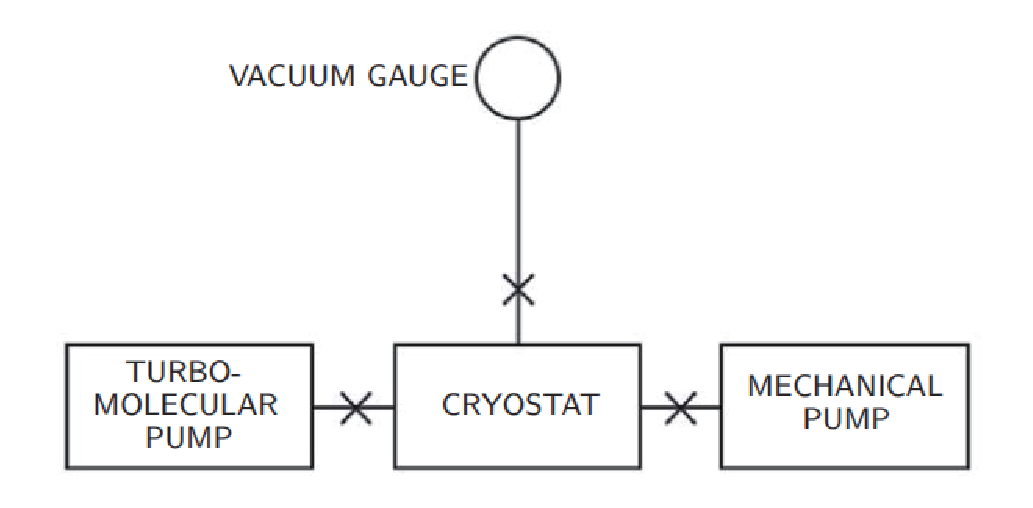
\includegraphics[scale=0.5]{chpt4/figs/fig4.16.eps}
	\caption{超导磁体运行中使用的典型真空泵系统框图。}
\end{figure}

\textbf{真空度量}

低温容器常用的两种真空度量方法是:1) 热电偶;2)电离计。下面是两种类型的简要描述。

\textbf{热电偶:} 热电偶度量的原理是在上面讨论的“低”压极限下压力对气体热导率的依赖关系。
热电偶节安装于连接到待测真空空间的管内,它的温度由加热器设定。
随压力变化的气体冷却热电偶;热电偶节电路的感应电流变化反映了真空压力。这种度量方法的应用
区间是$10^{-3}\sim 1$ torr,即机械泵覆盖的区间。

\textbf{电离计:} 对$\sim 10^{-6}$ torr和$10^{-4}$ torr之间的真空度,这也是多数低温容器
运行的区间,电离计广泛使用。有两种电离计:1) 热阴极;2) 冷阴极。

\textit{热阴极:} 这种度量器由加热丝(热阴极)、阳极、负偏置粒子采集板组成,上述部件都放置在
连接于待测量真空空间的管子内。电子从加热丝运动到阳极,与气体分子碰撞,产生离子化分子,被吸引到采集板。
测量电路测得相应的电流。由于分子是由电子离子化的,离子电流还依赖于撞击分子的电子数量:
精确的压力测量因而要求对加热丝电流的精细控制。
用于混合III低温容器的热电极度量器在磁体运行区间是关闭的,以最小化“加热器疲劳”。所谓加热丝疲劳,
是由加热丝的振荡运动产生的,源于加热丝供电电流和磁体边缘场的Lorentz相互作用。

\textit{冷阴极:} 也称为Philips或Penning度量,它使用一个冷阴极和两个平行阳极,磁场施加于阳极板法向,
每次开启($\sim 2$ kV)一个。冷阴极产生的少量电子于是被驱使沿螺旋轨迹交替运动向两个板中的一个。
这种配置有效的增加了少量电子和气体分子之间的碰撞几率。和加热丝不同,冷阴极不会“污染”气体也
不会为真空失效而损毁。但它的精确度要比热阴极差。

\subsection{讨论4.11:固态制冷工质/磁体}
\textbf{A. 设计和运行概念}

通常来说,超导磁体(LTS或HTS)在额定运行温度$T_{op}$ 和最高运行温度区间内应保持全超导并稳定运行。
相比于LTS,HTS的临界温度$T_c$高得多,差不多相同大小和场性能的HTS磁体的
运行区间$\Delta T_{op}$要比LTS大一个量级:典型的HTS值是$\Delta T_{op}$ > 1 K;而典型LTS值
$\Delta T_{op}$< 1 K (LTS和HTS磁体的温度裕度概念将在第6章讨论)。

FBML发展的设计/运行概念识别出了HTS磁体的大$\Delta T_{op}$,并将它与固体介质的大热容组合起来[4.30–
4.32]。在这个设计/运行概念中,$\Delta T_{op}$不再认为是LTS磁体允许的暂态偏离,而被看做磁体的新的机遇。

将运行温区扩展(主要是HTS,LTS也并非不可能)与增强的热容的组合提供了新的运行方式。下面将给出一个例子,
它在“传统”的设计/运行概念下,不管是不含固态介质的“干式”,或是浸泡于制冷剂中的“湿式”,抑或制冷剂迫冷的方式都不可行。注意,即使是固态介质冷却的磁体,主要冷源还是制冷机或者制冷回环器(讨论4.7)。
这样的磁体一般安装于磁体腔内,填充固体制冷工质。

\textbf{永久模式磁体应用}

这个设计/运行概念的一个应用是恒定场磁体,比如NMR和MRI这种通常运行在永久模式的。
这些磁体运行温度区间一般设计的很大,这个概念能让这种磁体在特定设计时间范围内,甚至在主要冷源
关闭或从冷体热解耦的情况下,都能维持恒定运行磁场。
冷源可能是故意关闭的,比如创造无冷源振动的测量环境,又如冷源维护,又如故障模式。

\textbf{B. 固体中的热扩散}

在均匀各向同性固体 (密度$\rho$,热导率$k$,比热$c_p$)中,通过固体的热扩散由它的热扩散系数 $D_{th}[\mathrm{m^2/s}]$描述:
\begin{equation}% 4.20
D_{th}=\frac{k}{\rho c_p}
\end{equation}

某点的暂态热在固体中传导$\delta_{sd}$距离的时间尺度于是为:
\begin{equation}% 4.21
\tau_{sd}=\frac{1}{D_{th}}(\frac{\delta_{sd}}{\pi})^2
\end{equation}

\textcolor{red}{表4.10}

表4.10列出了固氖 (SNe)、固氮(SN2)、铜(Cu)在4–60 K区间$\delta_{sd}$=10 mm时,$D_{th}$和对应的$\tau_{sd}$的近似值,数值基于$\rho(T)$, $c_p(T)$和$k(T)$数据[4.33–4.35]。
在这个温度区间,SN2的热扩散系数比铜小3-5个量级——相比固氮,热更容易传入铜。
例如,30 K时,如表4.10所列,对$\delta_{sd}$=10 mm,固氮中的$\tau_{sd}$=46 s,而在铜中只需1.3 ms。
不过,SN2单位体积可吸收的热量要比铜大得多。

\textbf{“缓慢”加热}

如果需要一定体积固态工质在合适的热扩散距离下吸收的热可以是缓慢吸收的,也即时间比$\tau_{sd}$长得多,
整个固体将维持近乎温度均匀。实际上,如前文所述,固体工质用于通常运行于永久模式的MRI和NMR是最佳的。
下面的问题4.3将研究,固体工质冷却的磁体的扩散距离1-2 cm的加热时间需要几个小时,整体固氮体积可以假定为
均匀温度分布的。

\textbf{暂态加热}

在快速暂态状态下,仅固体工质的一小薄层——注意
$\delta_{sd}\propto\sqrt{\tau_{sd}}$(方程4.21)——可有效吸收热量,多余热量将引起磁体绕组温升。
即使在这个极限下,尽管可能发生“热烧干”(下文),SN2业已被证明可有效抑制暂态加热下的HTS测试绕组温升[4.36, 4.37]。
最近,Kyoto大学的小组证明他们命名的“热干烧”现象在暂态热源表面和固体介质表面的接触面上产生了很大的温差[4.38–4.40]。下面将讨论热干烧和一个克服这个现象的解决方法。

\begin{figure}[htbp]
	\centering
	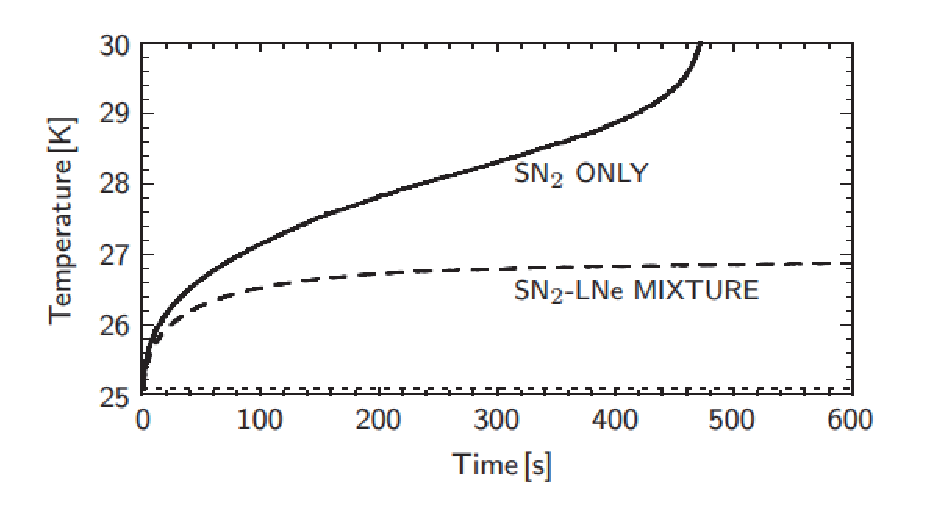
\includegraphics[scale=0.7]{chpt4/figs/fig4.17.eps}
	\caption{过流扰动下的HTS超导带的温度和时间关系。实线:仅由SN2冷却;虚线:由SN2-LN2混合物冷却;点线:初始温度25.1 K。}
\end{figure}


\textbf{C. “热烧干”}

Kyoto大学的Nakamura及其合作者试验展示了SN2的表面处于大的热流密度下,将发生热干烧[4.38–4.40]。
比如,对60 K的固氮,热干烧开始于能量密度$\sim 1.5\ \mathrm{W/cm^2}$。
很明显,接触面上的薄气膜是产生温度不连续的原因。

图4.17给出了过流扰动下的HTS超导带的温度和时间关系。扰动持续长达$\sim 600$ s。实线对应超导带仅与固氮
接触的运行方式;25.1 K的水平点线给出的是超导带和固氮的初始温度。
$\sim 400$ s之后,热流$14.3\ \mathrm{W/cm^2}$,对应温差($\Delta T$)超过3 K,发生热失控。如果
过流继续,将导致导体损毁。

\textbf{固氮-液氖混合物抑制热烧干}

Kyoto研究组证明固氮-液氖混合物——液氖占总体积的$\sim 1\%$——对抑制热烧干十分有效。
当然,LNe的使用将运行温区限制的更窄,大气压下为24.5-27.1 K。
图4.17中的虚线对应超导带由SN2-LNe混合物冷却的典型运行情况。
甚至在反复过流冲击下,他们观察到超导带温度仍维持在26.9 K,这是由LNe锚定的。
注意这里$Delta T<$ 2 K;更重要的是,至少对600 s,并无热失控发生迹象。
(两类测量方法中,“冷体”由作为系统冷源的制冷机持续冷却)

对液氮温区的应用,或许运行于65-77 K的固氩(SAr)和过冷液氮的混合物是一个提高固体工质固有劣热接触性质的有效方法。氖的熔点是83.8 K,沸点是87.3 K。



\subsection{问题4.3:固态制冷剂冷却的磁体}
本节我们处理固体工质冷却的磁体。

a) 使用图4.2给出的$C_p$ vs. $T$图,画出Cu、Pb、SNe、SN2的初始温度为4 K,终了温度为60 K,在1 W热输入下的$T(t)$与体积(1 L)的关系图;SNe终了温度为25 K。
假定加热期间体积内温度分布均匀。

b) 使用SN2的$T(t)$图——或者直接用图4.2——证明在恒定热输入0.25 W条件下,15 L的SN2从10 K加热到14 K需要$\sim 30$小时。忽略冷体中包括磁体本身在内的其他材料的热容,假定加热期间固氮内部温度分布均匀。

如讨论4.11论及,固态制冷工质冷却的磁体运行在一个大于LTS磁体典型$\sim 1$ K(或更小)温区是很有价值的。在一个SN2冷却的永久模式运行HTS磁体,例如,一个典型运行模式就是标称温度10 K下的有冷源运行。当冷源因有意消除噪声或意外断电而关闭,即它就和冷体热解耦,磁体将开始加热,
在温升$\Delta T_{op}$内保持运行磁场——对这个磁体该值为5 K。

为了充分利用冷体中固体制冷工质可提供的巨大热容,要求系统设计具有冷源关闭后冷体可自动与冷源热解耦的能力。

c) 15 L固氮置于冷体中,包围住外径896 mm(内径860 mm)、绕组高300 mm的磁体。
假设固氮是圆柱形, 内径$\simeq$ 896 mm,长300 mm,厚$\Delta r_{N2}$。(因为
冷体由足够厚的铜片构造,大部分热量从磁体内侧经冷体壁面通过固体导热到外壁面后进入冷体) 计算15 L固氮的$\Delta r_{N2}$,假定通过固氮层进入冷体的热量都是沿径向的。证明,对应这个
层厚度的热扩散系数$\sim 0.6$ s,它远比从10 K到15 K的加热时间小。

d) 证明如果装入的是固氖,b)中的冷体中的15 L制冷固氮工质可以折半。(因为SN2的单位体积价格
至少比SNe便宜$\sim 200$倍,除非必须用氖,否则还是用氮更合适)


e) 证明将这15 L固氮从15 K加热到60 K还需要大约80小时。
在15-60温度区间,假定向冷体的平均热输入是3.3 W。
忽略磁体升温到一定程度失超而由磁体中储存的磁能转化而来的热能。

f) 在15 K以上的加热过程中,当绕组的最高场部分达到比如说20 K,磁体开始失超,从而磁场下降。
对于这个绕组体积为15,000 $\mathrm{cm^3}$,储能量75 kJ的磁体,计算它的最终温度。
其初始温度20 K,假定在这整个暂态过程中全部磁能仅转换为绕组内的热能。
假定绕组能量转换结束时温度是均匀的,绕组的焓可由铜来近似。
因为总热能$\sim 1$ MJ被固氮吸收,从15 K升温至60 K,忽略e)中的附加75 kJ热能是合理的。

尽管磁体除了场衰减及随后这段时间都是温度均匀的,因为绕组内的场不均匀,故失超并非在绕组内部同时发生。
然而,场衰减仅持续几秒——这是基于实际HTS磁体的失超分析得到的。

g) 证明,在恒定热输入为10 W时,同样的HTS磁体需要$\sim 3$小时从初始运行温度30 K升温至最终的35 K。
假定b)中的假设都成立。

h) 在温区为35–40 K,同样的恒定热输入10 W,重复g),证明
同样是温升5 K,35.61 K的相变焓令温升时间翻倍。

固氮还可以用于稳定易于受到暂态扰动的HTS绕组。试验证实,一薄层($\sim 0.5$ mm)与Bi2223超导带
接触的固氮确实能够抑制导体在恒定传输电流过流脉冲下趋向正常态的温升[4.36, 4.37]。
由于固氮的不良热扩散性,仅一个薄层($\sim 0.5$mm)在吸收暂态能量耗散时是有效的。

i) 使用讨论4.11中的方程4.21,证明初始温度30 K,暂态恒定幅值(方波)的加热$\sim 0.1$ s时长,
在固氮层中扩散距离是0.4 mm。尽管加热过程固氮层升温,可使用30 K时的恒定值$D_{th}=2.4×10^{−3}\ \mathrm{cm^2/s}$ (表4.10中,$D_{th}=0.24\ \mathrm{mm^2/s}$).


j) 对于i)中的这个0.1 s暂态加热,证明固氮层被加热至35 K,可吸收的功率流为$4.2\ \mathrm{W/cm^2}$。

k) 讨论当被加热层必须在35.61 K经过固-固相变时,受到暂态加热的薄层固氮的有效性。
如表4.10的脚注所言,35.61 K时的固氮$D_{th}$理论上是0。

l) 讨论磁体在其允许运行温度区间(这里是10 K到15 K)的温升过程中,磁体的膨胀在何种程度上影响空间场的均匀性。

\subsubsection{问题4.3之解}
a) 图4.18给出了1 L体积Cu, Pb, SNe和SN2初始温度4.2 K,终了温度60 K(SNe是25 K)在恒定热输入1 W,$T(t)$图
——它还包括一条4.2 K水平点线,给出了1 L的4.2 K液氦挥发所需的时间。
从该图可清晰看出,在这些物质中,至少以体积算,4-25 K区间的SNe和25-60 K区间的SN2分别是
最好的热容增强剂。因为SNe的比密度($1.25\ \mathrm{g/cm^3}$@25 K)和SN2的比密度($1\ \mathrm{g/cm^3}$@25 K)
要比Pb($11.4\ \mathrm{g/cm^3}$)和Cu ($8.96\ \mathrm{g/cm^3}$)小一个量级,
热容增强剂在冷体中占有同样的额外体积时,这些固体工质都不仅能起到很好的效果,还仅增加了很小的系统质量。

以SN2为例,因为整个加热(4.2 K–60 K)过程需要$\sim 18$小时,
我们可以放心的说,扩散距离$\sim 10$ cm的1 L固体体积内的温度均匀分布假设是可行的。
均匀温度假设很明显对铜和铅都是合理的。

b) 从图4.18中,我们知道对于1 L的SN2,$T(t\simeq 400\ \mathrm{s})$ = 10 K,$T(t\simeq 2,150\ \mathrm{s})$ = 15 K。
对1 L的SN2,在1 W的热输入下,从10 K加热到15 K的时间为:$[\Delta t(10 \ \mathrm{K}\rightarrow 15\ \mathrm{K})]_{1\ \mathrm{L}}^{1\ \mathrm{W}}\simeq 1,750$ s = 0.486 h。在0.25 W的热输入下,15 L的固氮从10-15 K的加热时间$[\Delta t(10 \ \mathrm{K}\rightarrow 15 \ \mathrm{K})]_{15 \ \mathrm{L}}^{0.25\ \mathrm{W}}$由下式给出:
\begin{align*}% page260
[\Delta t(10\mathrm{K}\rightarrow 15\ \mathrm{K})]_{15\mathrm{L}}^{0.25\mathrm{W}}&=(\frac{1\mathrm{W}}{0.25\ \mathrm{W}})(\frac{15\mathrm{L}}{1\mathrm{l}})[\Delta t(10\mathrm{K}\rightarrow 15\mathrm{K})]_{1\mathrm{L}}^{1\mathrm{W}}\\\notag
&\simeq (4)(5)(0.486\mathrm{h})=29-30\mathrm{h}
\end{align*}

\begin{figure}[htbp]
	\centering
	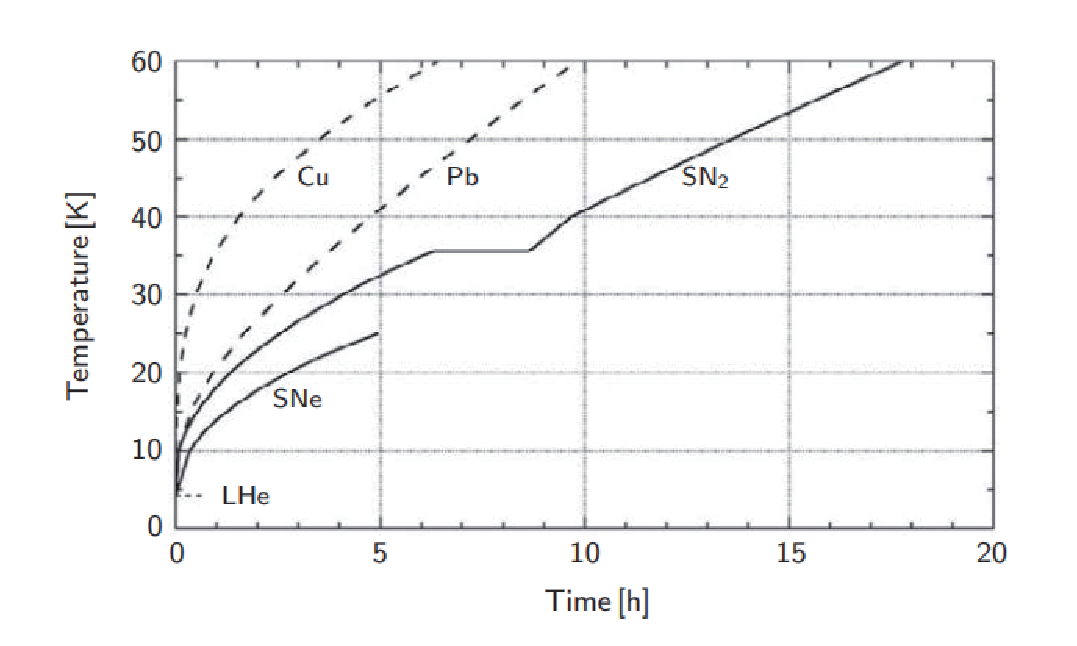
\includegraphics[scale=0.6]{chpt4/figs/fig4.18.eps}
	\caption{初始温度4.2 K,终末温度60 K,。。。$T(t)$。}
\end{figure}

另一种解法,我们可以直接使用图4.2,通过在10 K和15 K间对SN2应用$\int C_p(T)dT$计算$h(15\ \mathrm{K})−h(10\ \mathrm{K}) [\ \mathrm{J/cm^3}]$:
\begin{align*}% page260
h(15\ \mathrm{K})-h(10\ \mathrm{K})&\simeq\frac{C_p(10\ \mathrm{K})+C_p(15\ \mathrm{K})}{2}(15\ \mathrm{K}-10\ \mathrm{K})\\
&\simeq\frac{(0.175\ \mathrm{J/cm^3K}+0.475\ \mathrm{J/cm^3K} )}{2}(5\ \mathrm{K})\\
&\simeq 1.625\ \mathrm{J/cm^3}
\end{align*}

于是,在0.25 W的热输入下,15 L的固氮从10-15 K的加热时间$[\Delta t(10\ \mathrm{K}\rightarrow 15\ \mathrm{K})]_{15\ \mathrm{L}}^{0.25 W}$可由下式给出: 
\begin{equation*}% page260
[\Delta(10\ \mathrm{K} \rightarrow 15\ \mathrm{K})]_{15\ \mathrm{L}}^{0.25\ \mathrm{W}}=\frac{(15000\ \mathrm{cm^3})(1.625\ \mathrm{J/cm^3})}{(0.25\ \mathrm{W})(3600\ \mathrm{s/h})}\simeq 27.1\ \mathrm{h}\sim 30\ \mathrm{h}
\end{equation*}

c) 直径$D$,长度为$\ell$,壁厚$\Delta r_{N2}\ll D$的圆柱体内的固氮体积$V_{N2}$为:
\begin{equation*}% S3.1
\nu_{N2}=\pi D\ell\Delta r_{N2} \tag{S3.1}
\end{equation*}

代入$V_{N2}=15000\ \mathrm{cm^3},D=90\ \mathrm{cm},\ell= 30\ \mathrm{cm}$,有:
\begin{equation*}% S3.1
\Delta r_{N2}=\frac{\mu_{N2}}{\pi D\ell}=\frac{(15000\ \mathrm{cm^3})}{\pi(90\ \mathrm{cm})(30\ \mathrm{cm})}=1.8\ \mathrm{cm}
\end{equation*}

我们可以令$\Delta r_{N2}$=1.8 cm与方程4.21中的$\delta_{sd}$相等,代入10 K和15 K之间的大致平均值
$D_{th}\simeq 55\times10^{−2}\ \mathrm{cm^2/s}$解4.21,有:
\begin{equation}% 4.21
\tau_{sd}=\frac{1}{D_{th}}(\frac{\delta_{sd}}{\pi})^2
=\frac{1}{(55\times 10^{-2}\ \mathrm{cm^2/s})}(\frac{1.8\ \mathrm{cm}}{\pi})^2\sim 0.6\ \mathrm{s}
\end{equation}

扩散时间$\sim$ 0.6 s相比30小时的加热时间是很短的。于是,在15 L的SN2内的均匀温度分布假设是合理的。

d) 我们颠倒b)中给出的两种方法的顺序。即,使用图4.2中给出的固氖$C_p(T)$数据,计算SNe的$C_p(T)$曲线在10 K和15 K之间
与坐标轴围成的面积,有:
\begin{align*}% page260
h(15\ \mathrm{K})-h(10\ \mathrm{K})&\simeq\frac{C_p(10\ \mathrm{K})+C_p(15\ \mathrm{K})}{2}(15\ \mathrm{K}-10\ \mathrm{K})\\\notag
&\simeq\frac{(0.400\ \mathrm{J/cm^3K}+0.875\ \mathrm{J/cm^3K})}{2}(5\ \mathrm{K})\\\notag
&\simeq 3.2\ \mathrm{J/cm^3}
\end{align*}

在0.25 W热输入下,对15 L固氮从10 K到15 K的同样的加热时间$[\Delta t(10\ \mathrm{K}\rightarrow 15\ \mathrm{K})]_{15\ \mathrm{L}r}^{0.25\ \mathrm{W}}\simeq 27.1$ h下,固氖的体积$V_{Ne}(10\ \mathrm{K}\rightarrow 15\ \mathrm{K})$由下式给出:
\begin{equation*}% page261
V_{Ne}(10\ \mathrm{K} \rightarrow 15\ \mathrm{K})=\frac{(27.1\ \mathrm{h})(3600\ \mathrm{s/h} )(2.5\ \mathrm{W})}{(3.2\ \mathrm{J/cm^3})(1000 \ \mathrm{cm^3/L})}
\simeq 7.6\ \mathrm{L}\sim\frac{1}{2}\times 15\ \mathrm{L}
\end{equation*}

从图4.18中,我们看到对1 L固氖, $T(t\simeq 0.33\ \mathrm{h})=10\ \mathrm{K}$和$T(t\simeq
1.22\ \mathrm{h})=15\ \mathrm{K}$,有$[\Delta t(10\ \mathrm{K}\rightarrow 15\ \mathrm{K})]_{1\ \mathrm{L}}^{1\ \mathrm{W}}\simeq 0.89$ h。
对1 L的SN2,有:
$[\Delta t(10\ \mathrm{K}\rightarrow 15\ \mathrm{K})]_{1\ \mathrm{L}}^{1\ \mathrm{W}}\simeq 0.486$ h。
于是我们有:
\begin{equation*}% page261
V_{Ne}(10\ \mathrm{K}\rightarrow 15\ \mathrm{K})=\frac{(0.486\ \mathrm{h})}{0.89\ \mathrm{h}}(15\ \mathrm{L})\simeq 8.2 \ \mathrm{L}\simeq\frac{1}{2}\times(15\ \mathrm{L})
\end{equation*}

e) 从图4.18,我们看到对1 L的固氮,$T(t\simeq 0.6 h)=15 K$和$T(t\simeq 17.75\ \mathrm{h}) = 60\ \mathrm{K}$,
或者$[\Delta t(15\ \mathrm{K}\rightarrow 60\ \mathrm{K})]_{1\ \mathrm{L}}^{1\ \mathrm{W}}\simeq 17.15\ \mathrm{h}$。
对平均热输入3.3 W和15 L的SN2,有:
\begin{align*}% page261
[\Delta t(15\ \mathrm{K} \rightarrow 60\ \mathrm{K})]_{15\ \mathrm{L}}^{3.3\ \mathrm{W}}&=(\frac{15\ \mathrm{L}}{1\ \mathrm{L}})(\frac{1\ \mathrm{W}}{3.3\ \mathrm{W}})[\Delta t(15\ \mathrm{K}\rightarrow 60\ \mathrm{K})]_{1\ \mathrm{L}}^{1\ \mathrm{W}}\\
&\simeq(15)(0.303)(17.15\ \mathrm{h})\\
&=78\sim 80\ \mathrm{h}
\end{align*}

f) 在这转变中,能量以密度$5\ \mathrm{J/cm^3}[= (75\ \mathrm{kJ})/(15,000\ \mathrm{cm^3})]$流入初始温度为20 K的铜。
这样,我们可以由下式确定最终温度$T_f$:
\begin{equation*}% S3.2
\int_{20\ \mathrm{K}}^{T_i}[C_p(T)]_{cu}dT=5\ \mathrm{J/cm^3}
\end{equation*}

根据图4.2,我们发现S3.2满足$T_f\simeq 40$ K。

g) 使用图4.2中的SN2的$C_p(T)$数据,计算SN2的$C_p(T)$曲线在30 K和35 K之间
与坐标轴围成的面积,有
\begin{align*}% page261
h(35\ \mathrm{K})-h(30\ \mathrm{K})&\simeq\frac{C_p(30\ \mathrm{K})+C_p(35\ \mathrm{K})}{2}(35\ \mathrm{K}-30\ \mathrm{K})\\\notag
&\simeq\frac{(1.24\ \mathrm{J/cm^3 K}+1.55\ \mathrm{J/cm^3 K})}{2}(5\ \mathrm{K})\\\notag
&\simeq 7.0\ \mathrm{J/cm^3}
\end{align*}

于是我们有:
\begin{equation*}% page262
[\Delta t(30\ \mathrm{K} \rightarrow 35\ \mathrm{K})]_{15\ \mathrm{L}}^{10\ \mathrm{W}}=\frac{(15000\ \mathrm{cm^3})(7.0\ \mathrm{J/cm^3})}{(10\ \mathrm{W})(3,600\ \mathrm{s/h})}
\simeq 2.9\ \mathrm{h}\sim 3\ \mathrm{h}
\end{equation*}

h) 类似g),除了必须增加35.61 K时的能量吸收值$\Delta h(35.61 K)=8.2 J/cm3$。
同时,焓面积计算必须在两个温度区间进行:35–35.61 K和35.61–40 K。于是:
\begin{align*}% page262
h(40\ \mathrm{K})-h(35\ \mathrm{K})\simeq&\frac{C_p(35\ \mathrm{K})+C_p(35.61\ \mathrm{K})}{2}(35.61\ \mathrm{K}-35\ \mathrm{K}) \\\notag
&+\Delta h(35.61\ \mathrm{K})+\frac{C_p(35.61\ \mathrm{K})+C_p(40\ \mathrm{K})}{2}(40\ \mathrm{K}-35.61\ \mathrm{K})\\\notag
\simeq&\frac{(1.60\ \mathrm{J/cm^3 K}+1.62\ \mathrm{J/cm^3 K})}{2}(0.6\ \mathrm{K})\\\notag
&+8.2\ \mathrm{J/cm^3}+\frac{(1.29\ \mathrm{J/cm^3 K}+1.33\ \mathrm{J/cm^3 K})}{2}(4.39\ \mathrm{K})\\\notag
\simeq&0.98\ \mathrm{J/cm^3}+8.2\ \mathrm{J/cm^3}+5.75\ \mathrm{J/cm^3}\\\notag
\simeq& 14.9\ \mathrm{J/cm^3}\\\notag
\end{align*}

\begin{align*}
[\Delta t(30\ \mathrm{K} \rightarrow 35\ \mathrm{K})]_{15\ \mathrm{L}}^{10\ \mathrm{W}}=&\frac{(15,000\ \mathrm{cm^3})(14.9\ \mathrm{J/cm^3})}{(10\ \mathrm{W})(3,600\ \mathrm{s/h})}\\\notag
\simeq&6.2\sim 6\ \mathrm{h} \notag
\end{align*}

于是,在相同的温升5 K下,35.61 K时的额外的焓贡献令加热时间翻倍(2.1倍)。

i) 方程4.21用于计算$\tau_{sd}$ for $D_{th} = 2.4\times 10^{−3} \ \mathrm{cm^2/s}$和$\delta_{sd}=0.04\ \mathrm{cm}$,给出了$\tau_{sd}$实际是 $\sim 0.1$ s,即:
\begin{align}% 4.21
\tau_{sd}&=\frac{1}{D_{th}}(\frac{\delta_{sd}}{\pi})^2
\end{align}

j) 在30 K到35 K温度区间,0.067 s内可能注入0.04 mm厚的SN2层的最大功率流$p_{sd}$可由下式计算:
\begin{align*}% page 262
p_{sd}&=[h(35\ \mathrm{K})-h(30\ \mathrm{K})]\frac{\delta_{sd}}{\tau_{sd}}\\
&=(7.0\ \mathrm{J/cm^3})\frac{(0.04\ \mathrm{cm})}{(0.067\ \mathrm{s})}=4.2 \ \mathrm{W/cm^2}
\end{align*}

k) 如表4.10的脚注给出的,固氮在35.61 K下有$D_{th} = 0$。这是因为能量是由固体吸收而不是被扩散——8.2 $\mathrm{J/cm^3}$——
由于它经历相变,SN2热容近乎趋于无限大。
不过,暂态试验结果[4.36, 4.37]已经证明在扩展相变温度的很大的范围内,固氮的吸收暂态能量效果不减。

l) 因为绕组温升对磁体空间磁场均匀性的影响对NMR和MRI应用非常重要,我们将在讨论4.12中论及。



\subsection{讨论4.12:温升和场均匀性}
对NMR或MRI磁体,空间磁场均匀性是设计/运行的关键问题。
本节,我们将定量的计算在允许的温升区间内,加热何种程度上会影响磁场均匀性。
这里,我们在10–15 K区间内进行计算。

线性热膨胀系数$\alpha(T)$定义为:
\begin{equation}% 4.22
\alpha(T)=\frac{1}{L_o}(\frac{\partial L}{\partial T})_P
\end{equation}
式中,$L_0$是初始长度。下标$P$表示等压过程。在低温下,$\alpha(T)$可由下式给出:
\begin{equation}% 4.23
\alpha(T)=aT+bT^3
\end{equation}
基于铜在$0\le T\le 50$ K范围内试验得到的$\alpha(T)$图我们发现铜的$a$和$b$为:
$a_{Cu}= 5\times 10^{-9} K^{−2}$,$b_{Cu} = 3\times 10^{−11} K^{−4}$。
对于10 K和15 K之间的$\Delta T_{op} = 5$ K,我们可以计算铜的$\Delta L/L_0$。通过在10 K和15 K之间对方程4.23积分,可得
$(\Delta L/L_0)_{Cu}$。这里,铜被选做绕组材料的代表。
附录III的表A3.4列出了给定金属和非金属的平均线性热膨胀数据。我们可以导出,这些材料在20 K和80 K之间的膨胀变化百分比
是一个数量级的。于是,我们可以确认,选择铜来定量计算$\Delta L/L_0$没问题,于是:
\begin{equation}% 4.24
(\frac{\Delta L}{L_0}_{Cu})=\int_{10\ \mathrm{K}}^{15\ \mathrm{K}}(5\times 10^{-9}T+3\times 10^{-11}T^3)dT=0.62\times 10^{-6}
\end{equation}
线性变化发生在三个维度上。如果绕组在各方向等量膨胀,不会对均匀性有损害。
实际上,因为各绕组是各向异性的,磁场均匀性将会退降,但在何种程度上退降则取决于有多少介质是各向异性的;所以,
这个膨胀量是难于精确预测的。

注意到,所有材料的$\Delta L/L_0$不仅与$\Delta T_{op}$,且与初始温度有关。
增长。因此,由于固态介质冷却的NMR或MRI磁体存在潜在的在运行温度偏移下的磁场均匀性退降,故小心的保持他们的初始运行温度
在$\sim 20$ K之下,并保证$\Delta T_{op}$不大于10 K。

\subsection{讨论4.13:低温热测}
温度在超导磁体的导体、制冷、机械、保护和稳定性等关键设计与运行问题中举足轻重,这在
图1.6中可推知一二。于是,温度测量成为超导磁体运行和试验的一个不可或缺的条件。
这是一个很大的课题,有专著[4.41]或专门章节[4.42]研究它。
Rubin通过将近500多篇论文的钩沉,给出了一个1982-1997年间有关低温下热的测量的透彻的进展综述[4.43]。
这里,我们的范围仅涵盖测热传感器,而不是热测,深度为简介或略深。
特别的,我们讨论那些在超导磁体领域已可用并常用温度传感器;而不涉及仪器和校准技术——尽管它在热测领域
是重要课题。因为我们仅处理超导磁体和相关实验用的传感器,我们对测热传感器的讨论覆盖2-300 K温区。

\textbf{A. Kelvin温标}

1854年Kelvin提出将绝对领域作为热力学温标起点。1954年,kelvin (K)被选为热力学温度的单位,
定义为水的三相点温度(0.0100$\circ C$)的1/273.16。
这样,Celsius温标下水的冰点0$\circ C$对应273.15 K。K本身就表示了温标的单位,所以应该用
4.2 K或4.2 kelvins,而不能用4.2◦K或4.2度Kelvin。

\textbf{B. 要求}

如其他传感器一样,温度传感器有多种要求。这些要求包括(序号不代表重要性;括号内为期望):
1) 信号水平(高); 2) 灵敏度(高); 3) 响应时间(快,检测转变事件);4) 尺寸(小);
5) 磁场效应(小);6) DC偏置(零);和7) 费用(低)。其他想望的性能还包括可重复性、
稳定性和线性。尽管每一个传感器在小范围内对每一个变量都是线性函数,但明显在任意大范围内保持线性
是不可能的。随着基于计算机的数据采集技术的大规模使用,对线性的要求已不像过去那样高了。

\textbf{C. 温度传感器类型}

超导磁体及其试验中常用三种温度传感器:1) 二极管; 2) 电阻;和3) 热电偶。
气压量热计曾普遍使用,尤其是在实验室里,但现在已经罕用了。下面简要介绍上述三种温度传感器。

\textbf{二极管} 二极管等半导体器件的结电压在恒定电流的正向偏置下随温度降低而增加。
最广泛使用的二极管温度传感器是Si和GaAlAs结二极管;未校准的和校准的商业温度传感器均可购得。
校准的要比未校准的贵约4倍,价格的差异主要是由传感器的运行温区决定的。

\textbf{电阻} 两种温度系数的电阻温度传感器均有使用:基于半导体的负系数和基于金属的正系数
(一般来说,金属纯度高则传感器敏感性高,$\Omega/K$)。

负温度系数传感器包括germanium, carbon resistors, carbon-glass (主要用于磁场中)和ruthenium oxide。
正温度系数传感器包括platinum, platinum alloys和rhodium-iron。
zirconium oxynitride传感器,特别是Lake Shore Cryotronics, Inc的Cernox产品,越来越流行。
基于金属的传感器之中,基于纯铂的这一种最为突出,是高准确度要求下的必选;实际上,标准铂电阻
温度传感器定义了氢三相点13.8033 K到300 K以上的国际温度标准(International Temperature Standard)。

\textbf{温度谱}

图4.19给出了跨越100 pK到1 GK区间的温度谱。我们看到,超导磁体运行跨过不到2个log尺度,1 K–100 K。

\begin{figure}[htbp]
	\centering
	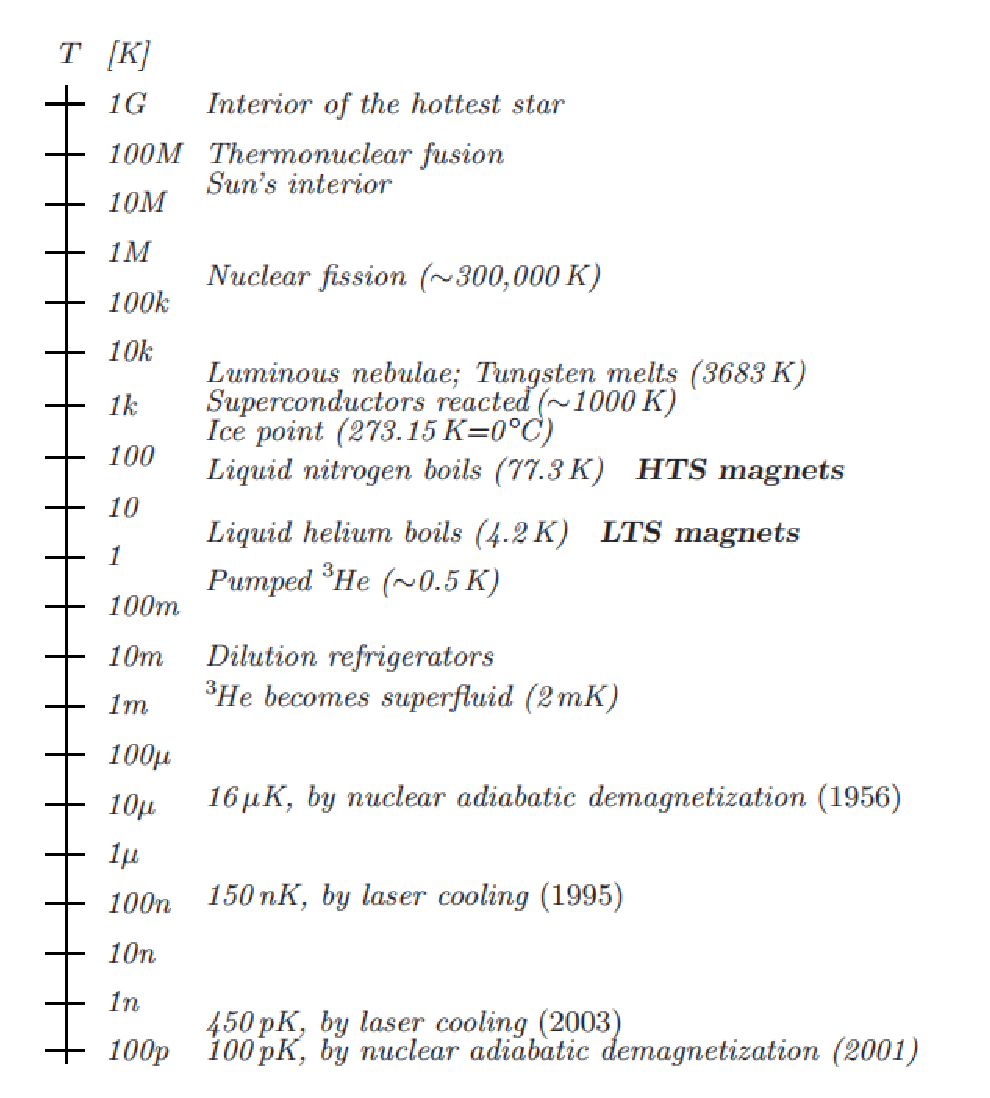
\includegraphics[scale=0.7]{chpt4/figs/fig4.19.eps}
	\caption{涵盖19个数量级的温度谱。}
\end{figure}

\textbf{热电偶} 对可容忍5\%温度不确定性的制冷应用——比如20 K下可容忍1 K——热电偶广泛使用。
这主要是由于热电偶符合上面列出的多项要求——尺寸小、响应快——比二极管和电阻温度传感器要好。
另外,热电偶也是这三种中最便宜的。

\textbf{D. 几种热传感器的信号水平和敏感性}

表4.11给出了6种常用热传感器的信号水平(V)和敏感性($\delta V/\delta T$)在2-300 K区间几个温度下的近似值。三种类型,每种选两个,二极管[4.44],电阻[4.44],热电偶[4.45]。
Note that these values are given here to demonstrate that both
signal levels and sensitivities vary over a wide range among thermometers and as
a “guide” in the selection process for appropriate sensors. 
这些传感器的商业渠道通常提供准确的“典型”数据;各校准的传感器都提供它自己的特定数据。
下面简要讨论表4.11中的各传感器,包括其磁场下的效应。

\textbf{评论,含磁场效应}

\textbf{Diode} 二极管热传感器,比如silicon和GaAlAs,在我们感兴趣的温区内具有最高的敏感性。
从表4.11中还可以推断出,传感器的V (T)曲线线性化很好,即在50-300 K区间,V大体上是随T线性减小的。
另一个吸引人之处是,大多数应用都可接受5\%的不确定性,仅依赖于制造商标准校准曲线的未校准的传感器
也是可用的。仅有的负面问题是它不适合用于磁场中,特别是低于60 K的温区内[4.45]。

\textbf{GaAlAs} 相比Si,GaAlAs有两处重要不同:1) V (T)具有更强的非线性;
2) 对$\sim 5$ T以内的磁场不敏感。

\textbf{Cernox} 尽管不如二极管敏感,仅次于Si的Cernox得到了广泛使用。
不像Si,它对磁场十分不敏感。制造商Lake Shore Cryotronics的数据[4.44]表明,
20 K下该传感器在20 T内的$\delta T/T$对磁场的不确定性小于0.2\%;误差随温度降低而增加,
在2 K时达到$\sim 5$\%。

\textbf{Platinum} 铂传感器在温度$\sim 40$ K以上对磁场十分不敏感:例如,40 K和5 T时,
$\delta T/T$是1.5\%,80 K和5 T时下降10倍[4.44]。

\textbf{E型热电偶} E型和Chromel-Au0.07\%Fe热电偶相比于其他四种传感器,信号水平和敏感性
都是最低的。以冰点($0^\circ$)为基准,E型在20 K的偏置电压为$\sim 11$ mV,
其敏感度仅为$\sim 10\mu$V/K。然而,当仅测量在特定运行点附近的温度变化时,它的准确度有很大提升。
同时,如果$\sim 5$\%的温度不确定性可以接受,并且需要大量传感器,那E型热电偶是一个极好的选择。
它的磁场的敏感性是中等的,比如在8 T磁场下,20 K时为2\%,45 K时<1\%[4.44]。

\textbf{AuFe(0.07\%)-Chromel} 所有的热电偶中,chromel-AuFe(0.07\%)具有最高的敏感性,于是
它最适合$\sim 20$ K之下的温度测量。不过,当AuFe(0.07\%)线有应变时,它的V (T) 值很容易偏离公开值[4.45]——它必须小心处理。
它对磁场的敏感性大致上要比E型热电偶高一个数量级。

\textbf{电容式热传感器}

尽管上面的讨论未涉及,但电容式热传感器,如strontium titanate传感器,因其对磁场依赖性很小也有所使用。
几种其他类型的基于玻璃或塑料材料的传感器在1 K以下温度测量上应用很多。

\subsection{讨论4.14:气冷铜电流引线}
对于浸于4.2 K液氦中的超导磁体,气冷铜引线会为制冷系统带来很大的热负荷。
优化的气冷铜引线的基本设计概念是令焦耳热和传导热大致相等,通过引线注入冷氦气带走这些热量。
气冷引线的工作开始于1960s,现在还在继续[4.47–4.52]。100 A-75 kA的气冷引线现在已可商业化购得。
最近,最大电流已经达到的100 kA水平[4.53]。这里,我们给出引线关键参数的解析表达式。

\textbf{A. 功率密度方程}

图4.20所示的载有额定电流$I_0$的气冷引线的微元体积$A\Delta z$内产生和流入的总功率$Q_{in}$为:
\begin{equation}% 4.25
Q_{in}=[Ak(T)\frac{dT}{dz}]_{z+\Delta z}+\dot{m}_Ic_p(T)T+\frac{\rho(T)I_{o}^{2}}{A}\Delta z
\end{equation}
式中,$z$是引线轴向距离,$z=0$位于引线的冷末端。
$k(T),A, \rho(T)$分别是引线(一般是铜)的热导率、有效截面积、电阻率。
$\.{m}_I$和$c_p(T)$分别是氦气的质量流量和比热。
氦气和引线之间的热传递假定为理想的。
$T$是$z$处引线和氦的温度。流出微元体积$A\Delta z$的总功率$Q_{out}$为:
\begin{equation}% 4.26
Q_{out}=[Ak(T)\frac{dT}{dz}]_z+\dot{m}_Ic_p(T)(T+\Delta T)
\end{equation}

稳态条件下,有$Q_{in}=Q_{out}$,于是:
\begin{equation}% 4.27
[Ak(T)\frac{dT}{dz}]_{z+\Delta z}-[Ak(T)\frac{dT}{dz}]_z-\dot{m}_Ic_p(T)\Delta T+\frac{\rho(T)I_{o}^{2}}{A}\Delta z=0
\end{equation}

\begin{figure}[htbp]
	\centering
	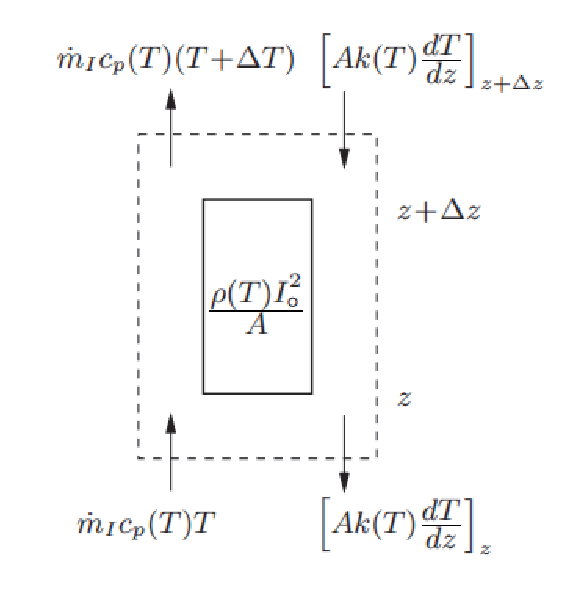
\includegraphics[scale=0.6]{chpt4/figs/fig4.20.eps}
	\caption{气冷引线的体积微元热平衡。}
\end{figure}

让方程4.27除以$\Delta z$,并令$\Delta z\rightarrow 0$,我们有:
\begin{equation}% 4.28
\frac{d[Ak(T)\frac{dT}{dz}]}{dz}-\dot{m}_Ic_p(T)\frac{dT}{dz}+\frac{\rho(T)I_{o}^{2}}{A}=0
\end{equation}

\textbf{B. 冷端热输入\&蒸发率}

在大电流极限下,即$|d[Ak(T)dT/dz]/dz|\ll\rho(T)I_O^2/A$时,方程4.28在$z=0$处有$T(0)=T_0$,可以简化为:
\begin{equation}% 4.29a
-\dot{m}_Ic_{p0}\frac{dT}{dz}\mid_{z=0}+\frac{\rho(T)I_{o}^{2}}{A}\simeq 0
\end{equation}
式中,$c_{p0}c_{p}(T_0)$,$\rho_0=\rho(T)$。由方程4.29a,我们可以解得$(dT/dz)_{z=0}$:
\begin{equation}% 4.29b
\frac{dT}{dz}\mid_{z=0}\simeq\frac{\rho_0I_{o}^{2}}{A\dot{m}_Ic_{p0}}
\end{equation}
因为$z=0$处$Q_{I_0}$完全是热传导,代入$k_0=k(T_0)$有:
\begin{equation}% 4.30
Q_{I_o}=Ak(T_0)\frac{dT}{dz}\mid_{z=0}=\frac{k_0\rho_0I_{0}^{2}}{\dot{m}_Ic_{p0}}
\end{equation}
进入液体的功率$Q_{I_0}$以$\.{m}_I$的速率令液体汽化:
\begin{equation}% 4.31a
\dot{m}_I=\frac{Q_{I_o}}{h_L}
\end{equation}
式中,$h_L$是液氦的汽化潜热[K/kg]。联立方程4.30和4.31a,解出$\.{m}_I$,有:
\begin{align*}% 4.31b
\dot{m}_I=I_o\sqrt{\frac{k_0\rho_0}{c_{p0}h_L}} \tag{4.31b}
\end{align*}
将方程4.31b给出的$\.{m}_I$代入方程4.30,解出$Q_{I_o}/I_o$,有:
\begin{equation}% 4.32a
\frac{Q_{I_o}}{I_o}=\sqrt{\frac{h_Lk_0\rho_0}{c_{p0}}}
\end{equation}

注意到,$Q_{I_o}$既不依赖于引线自底部($z = 0$)至顶部($z =\ell$)的有效长度$\ell$,
也不依赖于引线导体截面积$A$。不过,它正比于引线额定电流$I_o$。
如果引线载流$I<I_o$,冷端热输入将不再是$(I/I_o)Q_{I_o}$。

在这个讨论中,气冷引线冷端温度$T_0$假定为$T_0$=6 K之下的温度。
然而,由于经常需要提供高于磁体的液氦源,在实际气冷引线中,引线冷端($z = 0$)可能位于磁体顶部(和最低液位)以上——在一些情况下,要高出25 cm或更多。 然后,冷端在电气上和热上连接到超导体旁路的铜延伸段
,另一端($z<0$)插入液体中。超导体旁路(通常是铜/NbTi合物)载流通向磁体的电流$I_o$,
铜向液体传导热量$Q_{I_o}$。铜延伸段必须有足够的截面积以传导$Q_{I_o}$,甚至在其整个区段上无液氦,
也不应提高$T_0$过大,这样超导旁路才能以超导的状态载流$I_o$。


代入液氦的$h_L = 20.7 \times 10^3$ J/kg和$c_{p0}\simeq 5.26\times 10^3$ J/kg K;铜的
 $k_0 =600$ W/mK和$\rho_0\simeq 2.5\times 10^{-10}\ \mathrm{\Omega m}$,有:
\begin{align*}% 4.32b
\frac{Q_{I_o}}{I_o}&\simeq\sqrt{\frac{(20.7\times 10^3\ \mathrm{J/kg})(600\ \mathrm{W/mK})(2.5\times 10^{-10}\ \mathrm{\Omega m})}{5.26\times 10^3\mathrm{J/kgK}}}\\
&=7.7\times 10^{-4}\ \mathrm{W/A}=0.77\ \mathrm{mW/A}\sim 1\ \mathrm{mW/A} \tag{4.32b}
\end{align*}

对于一根优化的气冷引线,1 mW/A是估算进入液氦的热量的一个有用的典型值。
对一根额定运行于10 kA的引线,热负荷是$\sim $10 W;一对儿就是$\sim $20 W。

\textbf{C. 优化电流引线参数}

方程4.28的大电流近似为:
\begin{equation}% 4.33
\dot{m}_Ic_p(T)\frac{dT}{dz}+\frac{\rho(T)I_{o}^{2}}{A}=0
\end{equation}
对4.33,基于氦的从$T_0$到$T_{\ell}$温区的平均热容$c_p(T)\simeq \~{c}_p$,
在合适的区间对两端积分,解出$dT/\rho(T)$:
\begin{equation}% 4.34a
\int_{T_o}^{T_i}\frac{dT}{\rho(T)}=\int_{0}^{\ell}\frac{I_{o}^{2}dz}{A\dot{m}_I\tilde{c}_p}=\frac{I_{o}^{2}\ell}{A\dot{m}_I\tilde{c}_p}
\end{equation}
对铜,积分$\int_{T_0}^{T_\ell} dT/\rho(T)$可由下式近似给出:
\begin{align*}% 4.34b
\int_{T_o}^{T_i}\frac{dT}{\rho(T)}\simeq 1.2\times 10^{11}K\Omega m\tag{4.34b}
\end{align*}
上式中,$T_0$ = 6 K,$T_\ell$= 273 K。
将方程4.31b代入4.34a,假定$\~{c}_p\simeq c_{p0}$(这对氦是合理的),我们有:
\begin{align*}% 4.34c
\int_{T_o}^{T_i}\frac{dT}{\rho(T)}\simeq(\frac{I_{o}^{2}\ell}{Ac_{p0}})\frac{1}{I_0}\sqrt{\frac{c_{p0}h_L}{k_0\rho_0}} \tag{4.34c}
\end{align*}
我们用额定电流$I_o$、引线长度$\ell$和截面积$A$表示优化电流引线参数比$(I_o \ell/A)_{ot}\equiv \zeta_o$,有:
\begin{equation}% 4.35a
(\frac{I_o\ell}{A})_{ot} \equiv \zeta_o\simeq[\int_{T_0}^{T_i}\frac{dT}{\rho_(T)}]\sqrt{\frac{c_{p0}k_0 \rho_0}{h_L}}
\end{equation}
在上述方程中代入合适的数值,我们可以在数值上解出$\zeta_o$:
\begin{align*}
\zeta_o\simeq (1.2\times 10^11\ \mathrm{K/\Omega m})\sqrt{\frac{5.26XXX}{20.7XXX}}
\end{align*}
于是:
\begin{equation}% 4.35b
(\frac{I_o\ell}{A}_{ot})\simeq2.3\times10^7\ \mathrm{A/m}
\end{equation}
举例来说,对于=$I_o$=6 kA,$\ell$=38 cm,方程4.35b给出:$A\simeq 1\ \mathrm{cm^2}$。

\textbf{D. 静态热输入}

优化的引线无电流通过时的液氦蒸发率——称为静态蒸发率,$\.{m}_0$——仅取决于传导到氦中的热输入。
将$I_o$= 0代入方程4.28,我们有:
\begin{equation}% 4.36
A\tilde{k}\frac{d^2T}{dz^2}-\dot{m}_0\tilde{c}_p\frac{dT}{dz}=0
\end{equation}
式中,$\~{k}$和$\~{c}_p$分别是氦在温度区间$T_0$至$T_\ell$的平均热导率和平均比热。
\begin{equation}% 4.37
\tilde{k}=\frac{1}{T_\ell-T_0}\int_{T_0}^{T_\ell}k(T)dT
\end{equation}
表4.18给出了四种材料(G-10,不锈钢304,紫铜和黄铜)在三个制冷应用中常用温区的$\~{k}$值:
4–80 K;4–300 K;和80–300 K。

给定边界条件$T(z=0)=T_0$和$A\~{k}(dT/dz)_{z=0}=\.{m}_0 h_L$,$T(z)$可以表示为:
\begin{equation}% 4.38a
T(z)=T_0+\frac{h_L}{\tilde{c}_p}[\exp(\frac{\dot{m}_0\tilde{c}_pz}{A\tilde{k}})-1]
\end{equation}
于是:
\begin{align*}% 4.38b
T(\ell)\equiv T_\ell=T_0+\frac{h_L}{\tilde{c}_p}[\exp(\frac{\dot{m}_0\tilde{c}_p\ell}{A\tilde{k}})-1]\tag{4.38b}
\end{align*}
从方程4.38b中解出$\dot{m}_0\tilde{c}_p\ell/A\tilde{k}$,有:
\begin{equation}% 4.39a
\frac{\dot{m}_0\tilde{c}_p\ell}{A\tilde{k}}=\ln[\frac{\tilde{c}_p(T_\ell-T_0)}{h_L}+1]
\end{equation}
从方程4.39a中,我们可以解出$\.{m}_0$:
\begin{align*}% 4.39b
\dot{m}_0=\frac{\tilde{k}}{\tilde{c}_p}(\frac{A}{\ell})\ln[\frac{\tilde{c}_p(T_\ell-T_0)}{h_L}+1]\tag{4.39b}
\end{align*}
联立方程4.39b和$Q_0=\.{m}_0 h_L$,我们有:
\begin{equation}% 4.40a
Q_0=\frac{\tilde{k}h_L}{\tilde{c}_p}(\frac{A}{\ell})\ln[\frac{\tilde{c}_p(T_\ell-T_0)}{h_L}+1]
\end{equation}
对于优化的引线,有$(I_o \ell/A)_{ot}=\zeta_o$。于是:
\begin{align*}% 4.40b
Q_0=\frac{\tilde{k}h_L}{\tilde{c}_p}(\frac{I_o}{\zeta_o})\ln[\frac{\tilde{c}_p(T_\ell-T_0)}{h_L}+1]\tag{4.40b}
\end{align*}
对于优化的气冷铜引线,$Q_0$和$Q_{I_o}$的比值可由下式给出:
\begin{equation}% 4.41
\frac{Q_0}{Q_{I_o}}\frac{\tilde{k}}{\tilde{c}_p\zeta_o}\sqrt{\frac{h_Lc_{p0}}{k_0p_0}}\ln[\frac{\tilde{c}_p(T_\ell-T_0)}{h_L}+1]
\end{equation}
将$\~{k}$=660 W/mK;$\~{c}_p\simeq$5.2 kJ/kg K;$T_{\ell}$=300 K;$T_0$=4 K;以及
$\zeta_o\simeq2.3\times 10^7$  A/m代入方程4.11,有:
\begin{equation}% 4.42
\frac{Q_0}{Q_{I_o}}\simeq 0.69
\end{equation}
也即,气冷引线的静态挥发率大致上是引线通过额定电流时的挥发率的70\%。

\textbf{E. 优化电流引线的压降}

载流为$I_o$时,整条铜引线上的压降$V_o$为:
\begin{equation}% 4.43a
V_o=\frac{I_o}{A}\int_{0}^{\ell}\rho_{cu}dz
\end{equation}
有必要在引线长度$\ell$上作积分,因为铜的电阻率$\rho_{cu}$依赖于温度,也即随$z$变化。
方程4.43a可以改写为:
\begin{align*}% 4.43b
V_o=\tilde{\rho}_{cu}(\frac{I_o\ell}{A})_{ot}=\tilde{\rho}_{cu}\zeta_o \tag{4.43b}
\end{align*}
式中,
\begin{equation}% 4.44
\tilde{\rho}_{cu}=\frac{1}{\ell}\int_{0}^{\ell}\rho_{cu}dz\simeq\frac{1}{T_\ell-T_0}\int_{T_0}^{T_\ell}\rho_{cu}(T)dT
\end{equation}
方程4.44假设电流引线上的温度梯度是线性的。与方程4.43b和4.35b联立,其中$\~{\rho}_{cu}$的单位是$\Omega m$,我们有:
\begin{equation}% 4.45
V_o\simeq2.3\times 10^7\tilde{\rho}_{cu}\ \mathrm{V}
\end{equation}
也即,对任意额定电流优化的引线的$V_{ot}$是相同的。

对铜,$\~{\rho}_{cu}\sim 2.5\times 10^{−10}\ \mathrm{\Omega m}$ ($\sim$50 K之下)并且在
$\sim$50 K以上时与温度呈线性,273 K时为$1.75\times 10^{−8}\ \mathrm{\Omega m}$。
根据方程4.44,我们有:$\~{\rho}_{cu}\simeq 0.4\times 10^{-8}\ \mathrm{\Omega m}$。
优化引线在其额定电流运行时的压降与额定电流值无关;对铜引线,这个值$\sim$100 mV。
这样,100 A引线在载流为100 A时,或10 kA引线在载流为10 kA时,都有$V_o\sim$100 mV;
当热端被冷却——这在气冷引线中是很常见的——$V_{o}$将小于100 mV。
这个结论在数量级上与1 kA-30 kA的气冷铜引线的试验数据吻合很好[4.54]。

\textbf{F. 流体阻塞端的热负荷}

一旦发生冷却气体的流体阻塞,基于稳态解的优化引线设计方法就不再适用。
如果引线在无冷却的情况下持续通过额定电流$I_o$,引线可能发生“流体阻塞熔化”,通常是在热端附近。
优化引线微元的时变能量方程[W/m]为:
\begin{equation}% 4.46
AC_{cu}(T)\frac{dT}{dt}=\frac{d}{dz}[Ak(T)\frac{dT}{dz}]-\dot{m}_Ic_p(T)\frac{dT}{dz}+\frac{\rho_{cu}(T)}{A}I_{o}^{2}
\end{equation}
式中,$C_{cu}(T)$是引线金属(铜)的单位体积热容。
在无冷却($\.{m}_I=0$)和传导项为零(保守假设)时,方程4.46变为:
\begin{equation}% 4.47
AC_{cu}(T)\frac{dT}{dt}=\frac{\rho_{cu}(T)}{A}I_{o}^{2}
\end{equation}
优化的引线满足$(I_o\ell/A)=\zeta_o=2.3\times10^7$ A/m。于是:
\begin{equation}% 4.48
C_{cu}(T)\frac{dT}{dt}\frac{\rho_{cu}(T)\zeta_{o}^{2}}{\ell^2}
\end{equation}
因为流体阻塞熔化通常发生在近热端,我们用$C_o$(常数)替代$C_{cu}(T)$,以及
$\rho_{cu}(T)=\rho_o+\gamma_{cu}T$($\rho_o$和$\gamma_{cu}$都是常数):
\begin{equation}% 4.49
\frac{dT}{dt}=\frac{\rho_o\zeta_{o}^{2}}{C_o\ell^2}+\frac{\gamma_{cu}\zeta_{o}^{2}}{C_o\ell^2}T=\frac{\rho_o}{\gamma_{cu}\tau_\ell}+\frac{T}{\tau_\ell}
\end{equation}
引线的热常数$\tau_{\ell}$由下式给出:
\begin{equation}% 4.50
\tau_\ell=\frac{C_o\ell^2}{\gamma_{cu}\zeta_{o}^{2}}
\end{equation}
方程4.49的解为:
\begin{equation}% 4.51
T(t)=Ke^{t/\tau_\ell}-\frac{\rho_o}{\gamma_{cu}}
\end{equation}
式中,$K$是常数。方程4.51表明,在气流阻塞时,$T(t)$指数式升高,时间常数$\tau_\ell$。 因为$\tau_\ell$正比于$\ell^2$,更长的优化引线达到金属熔化温度的时间也更长。
因为$\zeta_o=(I_o \ell/A)$,我们还可以得出对同样额定电流的引线,粗的优化引线要比细的优化引线
更能抗受流体阻塞故障。

举例来说,对于一个优化的长为$\ell$=1 m的10 kA引线,其
$C_o=3.5\times 10^6\ \mathrm{J/m^3 K}$,$\gamma_{cu}=68\times 10^{-12}\ \mathrm{\Omega m/K}$,$(I_o \ell/A)\equiv\zeta_o=2.3\times 10^7$A/m,我们有:
\begin{align*}
\tau_\ell=\frac{(3.5\times 10^6\ \mathrm{J/m^3K})(1\ \mathrm{m})^2}{(68\times 10^{-12}\ \mathrm{\Omega m/K})(2.5\times 10^7\ \mathrm{A/m})^2}\sim 90\ \mathrm{s}
\end{align*}

注意,对优化的10 kA、$\ell$=1.4 m引线,$\tau_\ell$翻倍。

\subsection{讨论4.15:干式引线——正常金属和高温超导体}
对一个干式超导磁体,电流引线通常也必须运行于真空环境。
这里,我们讨论两类额定值为$I_o$的引线:1) 常规金属[4.55];2) 在其可用温度范围的HTS[4.56]。

\textbf{A. 正常金属}

单位引线长度上的稳态能量微分方程为:
\begin{equation}% 4.52
A\tilde{k}\frac{d^2T}{dz^2}+\frac{\tilde{\rho}I_{o}^{2}}{A}=0
\end{equation}
式中,$A$引线的有效截面积;$\~{k}$和$\~{\rho}$分别是金属的温度平均热导率和电阻率。
在$T(z = 0) = T_0$和$T(z =\ell) = T_\ell$边界条件下解方程4.52,我们得到了4.11,其中的冷端热输入$Q_{I_o}$可以导出:
\begin{equation}% 4.53
Q_{I_o}=A\tilde{k}\frac{dT}{dz}\mid_{z=0}=\tilde{k}(T_\ell-T_0)(\frac{A}{\ell})+\frac{\tilde{\rho}I_{o}^{2}}{2}(\frac{\ell}{A})
\end{equation}
将方程4.53对$\ell/A$微分,设$(I_o\ell/A)_{dr}$为零,我们可以得到以最小化$[Q_{I_o}]_{dr}$优化的
干式引线的$(I_o\ell/A)_{dr}$(方程4.12):
\begin{align*}% 4.12
(\frac{I_o\ell}{A})_{dr}=\sqrt{\frac{2\tilde{k}(T_\ell-T_0)}{\tilde{\rho}}}\tag{4.12}
\end{align*}
由方程4.12和4.53,我们得到$[Q_{I_o}]_{dr}$的表达式:
\begin{equation}% 4.54
[Q_{I_o}]_{dr}=I_o\sqrt{2\tilde{k}\tilde{\rho}(T_\ell-T_0)}
\end{equation}
代入$\~{k}$=600 W/mK和$\~{\rho}=1\times 10^{-8}\ \mathrm{\Omega m}$(紫铜在80-300 K区间的平均值),
方程4.54给出$[Q_{I_o}]_{dr}/I_o\simeq$ 45 mW/A;对黄铜,方程4.54给出 32 mW/A[4.19]。
也就是说,对于传导冷却的引线,黄铜要优于紫铜。

\textbf{B. HTS延伸}

YBCO发现之后,开始用HTS制作常规金属导线在冷端(小于$\sim$80 K)的延伸段[4.57, 4.58]。
HTS延伸段传入温度为$T_0$的磁体环境的热输入$[Q_{I_{hts}}]_{dr}$是理想热传导,由平均热导率$k_{hts}$,
截面积$A_{hts}$,长度$\ell_{hts}$和热端温度$T_{w_{hts}}$确定:
\begin{equation}% 4.55
[Q_{I_hts}]_{dr}=k_{hts}A_{hts}\frac{(T_{\omega_{hts}}-T_0)}{\ell_{hts}}
\end{equation}

在一个实际的常规金属/HTS引线中,常规金属的冷端热量(方程4.54给出,$T_0\simeq T_{w_{hts}}$),
一般由制冷机的一级冷头所吸收;二级冷头用于维持磁体在$T_0$。
同时,不论是块材还是带材制成的HTS引线都必须有保护;Bi2223带材电流引线的保护将在讨论8.5中涉及。
除了这里考虑的HTS引线,还存在气冷HTS引线变种,将在问题4.4-4.6中研究。


\subsection{问题4.4:气冷HTS电流引线——全超导型(FSV)}

气冷HTS电流引线与传导冷却HTS电流引线是最早实用化成功的HTS器件。
这项工作始于1989年,至今仍在进行[4.59–4.73]。HTS引线的额定电流现在已经达到了60 kA [4.69]和70 kA [4.74]。

这里,我们研究气冷HTS电流引线,特别是超导带制成的那种。对这种引线,HTS热端被热铆定于77–80 K;
在这个点上,HTS引线连接于气冷常规金属引线上以接入室温终端。
Hull将电流引线总共分为11类 [4.60]。其中就有全超导型(fully-superconducting version, FSV)气冷引线,
即在4.2K到77–80 K的整个温区都运行于超导态。
因为这种引线依赖于与氦气的对流冷却,它主要适用于浸泡于液氦中的超导磁体。

\begin{figure}[htbp]
	\centering
	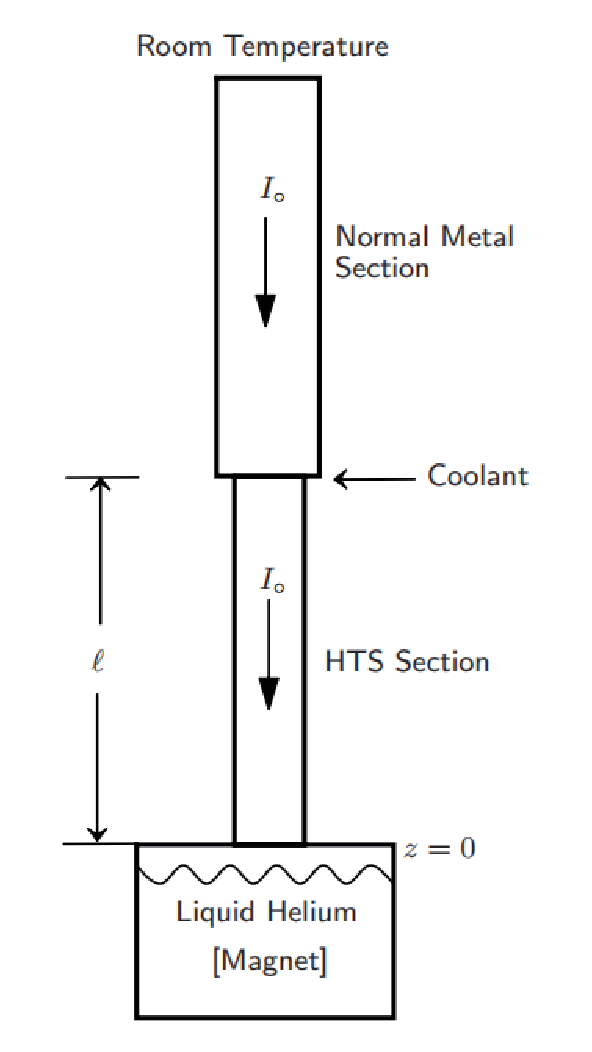
\includegraphics[scale=0.6]{chpt4/figs/fig4.21.eps}
	\caption{耦合于优化气冷常规金属的二元气冷引线。HTS引线从4.2 K的$z=0$处延伸至77-80 K的$z=\ell$。在$z=\ell$处,有额外制冷工质流入。}
\end{figure}

图4.21给出了我们要研究的气冷HTS引线的基本配置。它由$N_{fs}$条并联的HTS带组成,各带有效长度$\ell$。
HTS引线的额定电流$I_o$,冷端($z=0$)温度$T_0$,热端 ($z =\ell$)温度$T_\ell$。
HTS引线传导热量$Q_{in}$进入液氦,产生氦气的质量流量为$\~{m}_h$,这些氦气吸收引线长度$\ell$内的全部热量。

在$T_\ell$和室温之间,任何气冷HTS引线都必须耦合于以相同额定电流$I_o$优化的
气冷常规金属(通常是铜)引线上。
因为HTS引线的$Q_{in}$通常小于铜的对应值——这个$Q_{in}$的减小是采用HTS引线的唯一理由——
HTS部分产生的氦流量$\.{m}_h$对常规金属部分并不够用。
从而,常规金属气冷引线的冷端还要引入其他制冷剂,这在图4.21是可以看出来的。

由氦气冷却的HTS电流引线的微元的稳态时变能量方程:
\begin{equation}% 4.56
\frac{d}{dz}\left[[A_m]_{fs}k_m(T)\frac{dT}{dz}\right]-[\dot{m}_h]_{fs}c_p(T)\frac{dT}{dz}=0
\end{equation}
这里假定引线和氦气之间的热传递是理想的,两者之间温差为零。

方程4.56中,$[A_m]_{fs}$是FSV引线中HTS常规基底金属——如B92223带的Ag-Cu——的总截面积:
$[A_m]_{fs}=N_{fs} a_m$,其中$a_m$是各超导带的基底截面积;
$N_{fs}$是并联HTS带材数量;$k_m(T)$是基底金属的热导率;
$[\.{m}_h]_{fs}$是氦流量;$c_p(T)$是氦的比热。
我们分别令$k_m(T)=\~{k}$和$c_p(T)=\~{c}_p$,即令$k_m(T)$和$c_p(T)$均取$z=0$处的$T_0$至$z=\ell$处的$T_\ell$温区间的平均数。于是:
\begin{equation}% 4.57
[A_m]_{fs}\tilde{k}\frac{d^2T}{dz^2}-[\tilde{m}_h]_{fs}\tilde{c}_p\frac{dT}{dz}=0
\end{equation}
从方程4.57解出$T(z)$:
\begin{equation}% 4.58
T(z)=T_0+(\frac{T_\ell-T_0}{e^{[\alpha]_{fs}}-1})[e^{[\alpha]_{fs}(z/\ell)}-1]
\end{equation}
式中,$[\alpha]_{fs}$是无量纲数,定义为:
\begin{equation}% 4.59
[\alpha]_{fs}=\frac{[\dot{m}_h]_{fs}\tilde{c}_p\ell}{\tilde{k}[A_m]_{fs}}
\end{equation}

a) 证明,输入到氦池$(z=0)$的热量$[Q_{in}]_{fs}$为:
\begin{equation}% 4.60
[Q_{in}]_{fs}=\frac{\tilde{k}[A_m]_{fs}h_L}{\tilde{c}_p\ell}\ln\left[\frac{\tilde{c}_p(T_\ell-T_0)}{h_L}+1\right]
\end{equation}
式中,$h_L$是氦的汽化潜热。注意到$[Q_{in}]_{fs}$不仅正比于电流,而且由于$[A_m]_{fs}= N_{fs} a_m$,还正比于$N_{fs}$。这和气冷铜引线的$Q_{I_o}\propto I_o$是不同的。

b) 证明,铜引线$z =\ell$处传导到FSV引线的热量,即$[Q_{in}]_{fs}$和$[Q]_{fs}$之差,等于
氦气在$z=\ell(T_\ell)$和$z=0 (T_0)$间的焓差:
\begin{equation}% 4.61
[Q_\ell]_{fs}-[Q_{in}]_{fs}=[\dot{m}_h]_{fs}\tilde{c}_p(T_\ell-T_0)
\end{equation}

\subsubsection{问题4.4之解}
a) 利用方程4.58,我们可以首先解出$dT/dz|_0$。然后,$[Q_{in}]_{fs}$为:
\begin{align*}
[Q_{in}]_{fs}=\tilde{k}[A_m]_{fs}\frac{dT}{dz}\mid_0=[\dot{m}_h]_{fs}h_L \tag{S4.1}
\end{align*}
由方程4.58计算$dT/dz|_0$,将$[\alpha]_{fs}$代入方程4.59,有:
\begin{align*}
\tilde{k}[A_m]_{fs}\frac{dT}{dz}\mid_0&=\tilde{k}[A_m]_{fs}(\frac{T_\ell-T_0}{e^{[\alpha]_{fs}-1}})\frac{[\alpha]_{fs}}{\ell}\\
&=(\frac{T_\ell-T_0}{e^{[\alpha]_{fs}}-1})[\dot{m}_h]_{fs}\tilde{c}_p=[\dot{m}_h]_{fs}h_L\tag{S4.2}
\end{align*}
解出$e^{[\alpha]_{fs}}$:
\begin{align*}
e^{[\alpha]_{fs}}=\frac{\tilde{c}_p(T_\ell-T_0)}{h_L}+1 \tag{S4.3a}
\end{align*}
\begin{align*}
[\alpha]_{fs}=\ln\left[\frac{\tilde{c}_p(T_\ell-T_0)}{h_L}+1\right]\tag{S4.3b}
\end{align*}
联立方程4.59和S4.3b,有:
\begin{align*}
[\dot{m}_h]_{fs}=\frac{\tilde{k}[A_m]_{fs}}{\tilde{c}_p\ell}\ln\left[\frac{\tilde{c}_p(T_\ell-T_0)}{h_L}+1\right]\tag{S4.4}
\end{align*}
将S4.4代入S4.1,有:
\begin{align*}% 4.60
[Q_{in}]_{fs}=\frac{\tilde{k}[A_m]_{fs}h_L}{\tilde{c}_p\ell}\ln\left[\frac{\tilde{c}_p(T_\ell-T_0)}{h_L}+1\right] \tag{4.60}
\end{align*}

严格来说,方程4.60仅在系统制冷剂连续补液进而液位保持不变的条件下成立;如果不是这样,
$[\.{m}_h]_{fs}h_L$需要一个校正系数$(1−\rho_v/\rho_\ell)$[4.63],
其中$\rho_v$和$\rho_\ell$分别是气体和液体在的饱和密度。
4.2 K时,密度比是0.135:f$(1−\rho_v/\rho_\ell)$=0.865.

b) 上端在$z=\ell$处传导到引线中的热量$[Q_{\ell}]_{fs}$为:
\begin{align*}
[Q_\ell]_{fs}&=\tilde{k}[A_m]_{fs}\frac{dT}{dz}\mid_\ell=[\dot{m}_h]_{fs}\tilde{c}_p(\frac{T_\ell-T_0}{e^{[\alpha]_{fs}-1}})e^{[\alpha]_{fs}}\\ \tag{S4.5a}
&=[\dot{m}_h]_{fs}h_L\left[\frac{\tilde{c}_p(T_\ell-T_0)}{h_L}+1\right]\\
&=[\dot{m}_h]_{fs}\tilde{c}_p(T_\ell-T_0)+[\dot{m}_h]_{fs}h_L\tag{S4.5b}
\end{align*}
联立方程S4.1和S4.5b的外部项,有:
\begin{align*}% 4.61
[Q_\ell]_{fs}-[Q_{in}]_{fs}=[\dot{m}_h]_{fs}\tilde{c}_p(T_\ell-T_0v)\tag{4.61}
\end{align*}
方程4.61表明,三个功率项是平衡的。也即,$z=\ell$处进入引线的热量与$z=0$处流出引线的热量差
恰好等于氦气的热功率增加量。

\subsection{问题4.5:气冷HTS引线——电流共享型(CSV)}

这里我们研究气冷HTS电流引线,其中热端($T_\ell$) 的一小段设计运行于所谓的“电流共享”模式[4.75–
4.77]——电流共享将在第六章研究。电流共享型(CSV)的气冷HTS引线和问题4.4中研究的FSV型的额定电流相同。
图4.22给出了引线超导体的线性化$I_c(T)$图,其在$T_0 (z = 0)$时临界电流$I_{c0}$,
在$T_\ell(z=\ell)$时为$I_{c\ell}$。水平点线图还给出了引线的额定传输电流$I_o$。
如图指出的,电流共享开始的温度$T_{cs}$时,$I_c(T_{cs})=I_o$。
虚线给出了$I_o$流过超导体常规金属基底的部分。在$T_\ell$时,超导体载流$I_{c\ell}$,基底载流
$I_o-I_{c\ell}$。HTS引线的这个很小的部分产生焦耳热,必须用足够的氦将之带走。

\textbf{CSV的优势}

在相同的额定传输电流下,相比于FSV型,CSV型引线含有较少($N_{cs}$)的贵重HTS带材 ($N_{cs} <N_{fs}$)。
并且,如问题4.6讨论的6 kA引线所给出的,CSV引线的冷端的热输入要小于FSV的。

\textbf{超导段分析}($0\le z\le \ell_{cs}$)

我们首先分析这条CSV引线的超导部分。它位于温度为$T_0$的$z = 0$到温度为$T_{cs}$的$z =\ell_{cs}$之间。
由归一化$z$($\xi\equiv z/\ell$)表示的温度$T(\xi)$以及材料物性常数与方程4.58类似。于是:
\begin{equation}% 4.62
T(\xi)=(\frac{T_{cs}-T_0}{e^{[\alpha_\ell]_{cs}\xi_{cs}}-1})(e^{[\alpha_\ell]_{cs}\xi}+\frac{e^{[\alpha_\ell]_{cs}\xi_{cs}T_0-T_{cs}}}{T_{cs}-T_0})
\end{equation}
由于$[A_m]_{cs}=N_{cs}a_m$,$[\alpha_{1}\ell]_{cs}$可由下式给出:
\begin{equation}% 4.63
[\alpha_\ell]_{cs}\equiv\frac{[\dot{m}_h]_{cs}\tilde{c}_p\ell}{\tilde{k}[A_m]_{cs}}
\end{equation}

\begin{figure}[htbp]
	\centering
	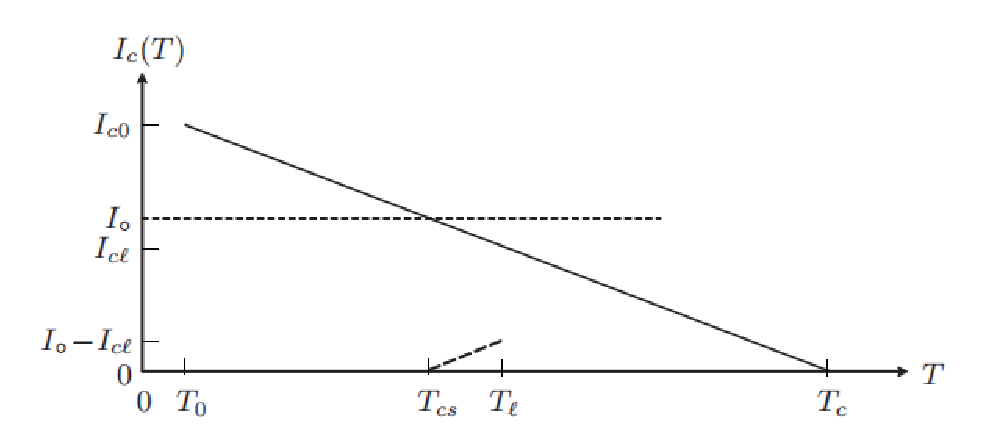
\includegraphics[scale=0.7]{chpt4/figs/fig4.22.eps}
	\caption{$I_c(T)$图(实线),对HTS温区内近似为线性。水平点线是引线的额定电流$I_o$。
		虚线给出了在电流分享区域通过母体的电流$I_o-I_c(T)$。}
\end{figure}

a) 证明在方程4.62中,$T(\xi=0)=T_0$,以及$T(\xi=\xi_{cs}=T_{cs}$。
	
b) 证明CSV引线的$z=0$处的热输入$[Q_{in}]_{cs}$由下式给出:
\begin{equation}% 4.64
[Q_{in}]_{cs}=\frac{\tilde{k}[A_m]_{cs}h_L}{\tilde{c}_p\ell_{cs}}\ln\left[\frac{\tilde{c}_p(T_{cs}-T_0)}{h_L}+1\right]
\end{equation}
我们将在问题4.6中看到,实践中数值上处理时,$\ell_{cs}$和$T_{cs}−T_0$分别近似等于
FSV中对应的$\ell$和$T_\ell−T_0$。于是,$[Q_{in}]_{cs}<[Q_{in}]_{fs}$主要源自$[A_m]_{cs} < [A_m]_{fs}$。在推导4.64过程中,同时证明$[\alpha_\ell]_{cs}$由下式给出:
\begin{subequations}
	\begin{align*}
e^{[\alpha_\ell]_{cs}\xi_{cs}}&=\frac{\tilde{c}_p(T_{cs}-T_0)}{h_L}+1\\
[\alpha_\ell]_{cs}&=\frac{1}{\xi_{cs}}\ln\left[\frac{\tilde{c}_p(T_{cs}-T_0)}{h_L}+1\right]
	\end{align*}
\end{subequations}

\textbf{电流分享段分析}($\ell\lg z\le \ell$)

在电流分享区域,即温度为$T_{cs}$的$z=\ell_{cs}$处至温度为$T_\ell$的$z=\ell$处,
假定材料物性为常数的导体单位长度功率方程为:
\begin{equation}% 4.66
\tilde{k}[A_m]_{cs}\frac{d^2T}{dz^2}-[\dot{m}_h]_{cs}\tilde{c}_p\frac{dT}{dz}+\frac{\tilde{\rho}_xI_o(I_o-I_{c\ell})}{[A_m]_{cs}(T_\ell-T_{cs})}(T-T_{cs})=0
\end{equation}
方程4.66中的第三项给出了运行于电流分享模式的CSV引线在这个区段产生的焦耳热。
$\~{\rho}_x$是这个区域内引线的温度平均电阻率。
考虑边界条件$T(\ell_{cs})=T_{cs}$和$T(\ell)=T_\ell$,并用$\ell$归一化$z$,$\xi\equiv z/\ell$,
我们得到在$\xi_{cs}\le\xi\le 1$范围内:

\begin{equation}% 4.67
T(\xi)=T_{cs}+\frac{(T_\ell-T_{cs})}{e^{\frac{[\alpha_\ell]_{cs}}{2}}\sin\beta_{cs}(1-\xi_{cs})}
\end{equation}
式中,$\beta_{cs}$也是无量纲数,由下式给出:
\begin{equation}% 4.68a
\beta_{cs}=\sqrt{\frac{\tilde{\rho}_xI_o(I_o-I_{c\ell})\ell^2}{\tilde{k}[A_m]_{cs}^{2}(T_\ell-T_{cs})}-\frac{1}{4}(\frac{[\dot{m}_h]_{cs}\tilde{c}_p\ell}{\tilde{k}[A_m]_{cs}})^2}
\end{equation}
联立方程4.68a和4.63,有:
\begin{equation}% 4.68b
\beta_{cs}=\sqrt{\frac{\tilde{\rho}_xI_o(I_o-I_{c\ell})\ell^2}{\tilde{k}[A_m]_{cs}^{2}(T_\ell-T_{cs})}-\frac{1}{4}[\alpha_\ell]_{cs}^{2}}
\end{equation}
联立4.68b和4.65b,我们有:
\begin{equation}% 4.68c
\beta_{cs}=\sqrt{\frac{\tilde{\rho}_xI_o(I_o-I_{c\ell})\ell^2}{\tilde{k}[A_m]_{cs}^{2}(T_\ell-T_{cs})}-\frac{1}{4}\{\frac{1}{\xi_{cs}}\ln\left[\frac{\tilde{c}_p(T_{cs}-T_0)}{h_L}+1\right]\}^2}
\end{equation}

c) 令方程4.62和方程4.67分别给出的热传导相等,两者都有$\xi_{cs}=\ell_{cs}/\ell$,证明
$\xi_{cs}$可以写为:
\begin{equation}% 4.69
[\alpha_\ell]_{cs}e^{\frac{[\alpha_\ell]_{cs}(1+\xi_{cs})}{2}}=\frac{\beta_{cs}}{\sin\beta_{cs}(1-\xi_{cs})}\left[\frac{\tilde{c}_p(T_\ell-T_{cs})}{h_L}\right]
\end{equation}
联立4.65a,4.65b和4.69,并注意到:
\begin{subequations}
	\begin{align*}
e^{\frac{[\alpha_\ell]_{cs}}{2}}&=\left[\frac{\tilde{c}_p(T_{cs}-T_0)}{h_L}+1\right]^{1/(2\xi_{cs})}\\
e^{\frac{[\alpha_\ell]_{cs}\xi_{cs}}{2}}&=\left[\frac{\tilde{c}_p(T_{cs}-T_0)}{h_L}+1\right]^{1/2)}
	\end{align*}
\end{subequations}
我们得到:
\begin{equation}% 4.71
\frac{1}{\xi_{cs}}\left[\frac{h_L}{\tilde{c}_p(T_\ell-T_{cs})}\right]\ln\left[\frac{\tilde{c}_p(T_{cs}-T_0)}{h_L}+1\right]\left[\frac{\tilde{c}_p(T_{cs}-T_0)}{h_L}+1\right]
\end{equation}

对于一组CSV引线参数——$\~{\rho}_x, \~{k}, [A_m]_{cs}, I_o, I_{c\ell}$——方程4.71中
唯一不知道的参数是$\xi_{cs}$。因为$\beta_{cs}$(方程4.68c)中唯一不知道的参数也是$\xi_{cs}$,
$\xi_{cs}$必须同时满足方程4.68c和4.71。

d) 证明在该CSV引线的整个超导段 ($0\le z\le \ell_{cs}$),三个功率项是平衡的: 
\begin{equation}% 4.72
[Q_{\ell_{cs}}]_{cs}-[Q_{in}]_{cs}=[\dot{m}_h]_{cs}\tilde{c}_p(T_{cs}-T_0)
\end{equation}
式中,$[Q_{\ell_{cs}}]$是在$z=\ell_{cs}$进入全超导段的传导热。

e) 证明在电流共享区域,四个功率项——在$z =\ell$处进入CSV引线的传导热$[Q_\ell]_{cs}$;
区域内产生的总焦耳热耗散$Q_j$;在$z =\ell_{cs}$处流出引线的传导热$[Q_{\ell_{cs}}]$;以及对流冷量$\.{m}_h \~{c}_p (T_\ell-T_{cs})$——是平衡的。
\begin{equation}% 4.73
[Q_\ell]_{cs}+Q_j-[Q_{\ell_{cs}}]_{cs}=[\dot{m}_h]_{cs}\tilde{c}_p(T_\ell-T_{cs})
\end{equation}

f) 证明:
\begin{equation}% 4.74
[Q_\ell]_{cs}+Q_j-[Q_{\ell_{cs}}]_{cs}=[\dot{m}_h]_{cs}\tilde{c}_p(T_\ell-T_0)
\end{equation}
即,在整个CSV引线范围内,能量是平衡的。


\subsubsection{问题4.5之解}
a) 将$\xi=0$代入方程4.62,有:
\begin{align*}
T(0)&=\left(\frac{T_{cs}-T_0}{e^{[\alpha_{1}\ell]_{cs}\xi_{cs}}-1}\right)\left(1+\frac{e^{[\alpha_{1}\ell]_{cs}\xi_{cs}}T_0-T_{cs}}{T_{cs}-T_0}\right)\\
&=\left(\frac{T_{cs}-T_0}{e^{[\alpha_{1}\ell]_{cs}\xi_{cs}}-1}\right)\left[\frac{T_0({e^{[\alpha_{1}\ell]_{cs}\xi_{cs}}-1})}{T_{cs}-T_0}\right]=T_0 \tag{S5.1}
\end{align*}
类似的,将$\xi=\xi_{cs}$代入方程4.62,有:
\begin{align*}
T(\xi_{cs})&=(\frac{T_{cs}-T_0}{e^{[\alpha_\ell]_{cs}\xi_{cs}}-1})(e^{[\alpha_\ell]_{cs}\xi_{cs}}+\frac{e^{[\alpha_\ell]_{cs}\xi_{cs}}T_0-T_{cs}}{T_{cs}-T_0})\\ &=(\frac{T_{cs}-T_0}{e^{[\alpha_\ell]_{cs}\xi_{cs}}-1})[\frac{T_{cs}(e^{[\alpha_\ell]_{cs}\xi_{cs}}-1)}{T_{cs}-T_0}]=T_{cs}
\end{align*}

b) 我们有:
\begin{equation}
[Q_{in}]_{cs}=\frac{\tilde{k}[A_m]_{cs}}{\ell}\frac{dT}{d\xi}\mid_{\xi=0}
\end{equation}
式中,$dT/d\xi$由方程4.62给出的$T(\xi)$计算。于是:
\begin{equation}
[Q_{in}]_{cs}=\frac{\tilde{k}[A_m]_{cs}}{\ell}(\frac{T_{cs}-T_0}{e^{[\alpha_\ell]_{cs}\xi_{cs}}-1})[\alpha_\ell]_{cs}\ell_{cs}=[\dot{m}_h]_{cs}h_L
\end{equation}
联立方程4.63和S5.4给出的$[\alpha_{1}\ell]_{cs}$我们得到:
\begin{equation}% 4.65a
e^{[\alpha_\ell]_{cs}\xi_{cs}}=\frac{\tilde{c}_p(T_{cs}-T_0)}{h_L}+1
\end{equation}
\begin{equation}% 4.65b
[\alpha_\ell]_{cs}=\frac{1}{\xi_{cs}}\ln[\frac{\tilde{c}_p(T_{cs}-T_0)}{h_L}+1]
\end{equation}
最后,联立方程S5.3和4.65b,并注意到$xi_{cs}\ell=\ell_{cs}$,我们有:
\begin{equation}% 4.64
[Q_{in}]_{cs}=\frac{\tilde{k}[A_m]_{cs}h_L}{\tilde{c}_p\ell_{cs}}\ln[\frac{\tilde{c}_p(T_{cs}-T_0)}{h_L}+1]
\end{equation}
虽然4.60给出的FSV的$\ell_{cs}<\ell$,$[Q_{in}]_{cs}<[Q_{in}]_{fs}$,由于$[A_m]_{cs}/\ell_{cs}$
通常更小,最多也就是FSV的$[A_m]_{fs}/\ell$的$\sim 80\%$。


c) 我们可以令方程4.62导出的与方程4.67导出的温度斜率相等,解出$\xi_{cs}$。两者都有$\xi_{cs}=\ell_{cs}/\ell$。
\begin{equation}
\frac{dT}{d\xi}\mid_{\ell_{cs}}=\frac{[\alpha_\ell]_{cs}e^{[\alpha_\ell]_{cs}\xi_{cs}}(T_{cs}-T_0)}{(e^{[\alpha_\ell]_{cs}\xi_{cs}}-1)}
\end{equation}
\begin{equation}
\frac{dT}{d\xi}\mid_{\ell_{cs}}=\frac{\beta_{cs}e^{\frac{[\alpha_\ell]{cs}}{2}}(T_\ell-T_{cs})}{e^{\frac{[\alpha_\ell]_{cs}}{2}}\sin\beta_{cs}(1-\xi_{cs})}
\end{equation}

令S5.5a和S5.5b相等,有:

\begin{align*}
\frac{[\alpha_\ell]_{cs}e^{[\alpha_\ell]_{cs}\xi_{cs}}(T_{cs}-T_0)}{(e^{[\alpha_\ell]_{cs}\xi_{cs}}-1)}
=\frac{\beta_{cs}e^{\frac{[\alpha_\ell]_{cs}\xi_{cs}}{2}}(T_\ell-T_{cs})}{e^{\frac{[\alpha_\ell]_{cs}}{2}}\sin\beta_{cs}(1-\xi_{cs})} \tag{S5.6}
\end{align*}
方程S5.6可以重新排列,并与方程4.70联立得到4.71:

d) 从方程S5.5a,我们可以计算$[Q_{\ell_{cs}}]_{cs}$:
\begin{align*}
[Q_{\ell_{cs}}]_{cs}=\frac{\tilde{k}[A_m]_{cs}}{\ell}\frac{dT}{d\xi}\mid_{\ell_{cs}} 
=\tilde{k}[A_m]_{cs}\frac{[\alpha_\ell]_{cs}e^{[\alpha_\ell]_{cs}\xi_{cs}}(T_{cs}-T_0)}{\ell(e^{[\alpha_\ell]_{cs}\xi_{cs}}-1)} \tag{S5.7}
\end{align*}
由方程4.63中给出的$[\alpha_\ell]_{cs}$以及方程4.70b中得出的$e^{[\alpha_\ell]_{cs}\xi_{cs}}$,我们可以得到:
\begin{align*}
[Q_{\ell_{cs}}]_{cs}&=\tilde{k}[A_m]_{cs}\frac{[\dot{m}_h]_{cs}\tilde{c}_p\ell}{\tilde{k}[A_m]_{cs}}\times\frac{\left[ \frac{\tilde{c}_p(T_{cs}-T_0)}{h_L}+1\right] (T_{cs}-T_0)}{\ell\left[\frac{\tilde{c}_p(T_{cs}-T_0)}{h_L}\right]} \\
&=[\dot{m}_h]_{cs}h_L\left[ \frac{\tilde{c}_p(T_{cs}-T_0)}{h_L}+1\right] \tag{S5.8}
\end{align*}
因为$[Q_{in}]_{cs}=[\.{m}_h]_{cs} h_L$,联立方程S5.8,有:
\begin{equation}% 4.72
[Q_{\ell_{cs}}]_{cs}-[Q_{in}]_{cs}=[\dot{m}]_{cs}\tilde{c}_p(T_{cs}-T_0)
\end{equation}
也即,在CSV引线的整个超导短,能量是平衡的。

e) 在$z=\ell$处传导至引线的热量$[Q_\ell]_{cs}$可由方程4.67计算:
\begin{align*}
[Q_\ell]_{cs}=&\frac{\tilde{k}[A_m]_{cs}}{\ell}\frac{dT}{d\xi}\mid_\ell=\frac{\tilde{c}[A_m]_{cs}(T_\ell-T_{cs})}{\ell e^{[\alpha_\ell]_{cs}}\sin\beta_{cs}(1-\xi_{cs})} \\
&\times e^{[\alpha_\ell]_{cs}}[\frac{1}{2}[\alpha_\ell]_{cs}\sin\beta_{cs}(1-\beta_{cs})+\beta_{cs}\cos\beta_{cs}(1-\xi_{cs})] \\
=&\frac{\tilde{c}[A_m]_{cs}(T_\ell-T_{cs})}{\ell}[\frac{1}{2}[\alpha_\ell]_{cs}+\beta_{cs}\cot\beta_{cs}(1-\xi_{cs})] \tag{S5.9}
\end{align*}

在$z=\ell_{cs}$处传导出的热量$[Q_{\ell_{cs}}]_{cs}$可由方程S5.5b计算:
\begin{align*}
[Q_{\ell_{cs}}]_{cs}&=\frac{\tilde{k}[A_m]_{cs}}{\ell}\frac{dT}{d\xi}\mid_{\ell_{cs}}\\
&=\frac{\tilde{c}[A_m]_{cs}(T_\ell-T_{cs})}{\ell}\left[\beta_{cs}\frac{e^{\frac{[\alpha_\ell]_{cs}\xi_{cs}}{2}}}{e^{\frac{[\alpha_\ell]_{cs}}{2}}\sin\beta_{cs}(1-\xi_{cs})}\right]
\end{align*}

将方程4.67给出的以$\xi=z/\ell$表示的$T(\xi)$代入方程4.66左侧的最后一项,并对其在$\xi=\xi_{cs}$
和$\xi=1$间积分,可以得到$Q_j$:
\begin{align*}
	Q_j=\frac{\tilde{\rho}_x I_o(I_o-I_{c\ell})\ell}{[A_m]_{cs}e^{\frac{[\alpha_\ell]_{cs}}{2}\sin\beta_{cs}(1-\xi_{cs})}}\int_{xi_{cs}}^{1} e^{\frac{[\alpha_\ell]_{cs}}{2}\xi}\sin\beta_{cs}(\xi-\xi_{cs})d\xi \tag{S5.11}
\end{align*}
令$x=\xi-\xi_{cs}$,积分S5.11,有:
\begin{subequations}
\begin{align*}
Q_j=&
\frac{4\tilde{\rho}_xI_o(I_o-I_{c\ell})\ell e^{\frac{[\alpha_\ell]_{cs}\xi_{cs}}{2}}}{[A_m]_{cs}e^{\frac{[\alpha_\ell]_{cs}}{2}\sin\beta_{cs}(1-\xi_{cs})([\alpha_\ell]_{cs}^{2}+4\beta_{cs}^{2})}} \\\notag
&\times\mid e^{\frac{[\alpha_\ell]_{cs}}{2}x}\left(\frac{[\alpha_\ell]_{cs}}{2}\sin\beta_{cs}x-\beta_{cs}\cos\beta_{cs}x\right)\mid_{0}^{1-\xi_{cs}} \\\tag{S5.12a}
=&\frac{4\tilde{\rho}_xI_o(I_o-I_{c\ell})\ell}{[A_m]_{cs}e^{\frac{[\alpha_\ell]_{cs}}{2}}\sin\beta_{cs}(1-\xi_{cs})([\alpha_\ell]_{cs}^{2}+4\beta_{cs}^{2})} \\\notag
&\times\left[\frac{[\alpha_\ell]_{cs}}{2}e^{\frac{[\alpha_\ell]_{cs}}{2}}\sin\beta_{cs}(1-\xi_{cs})-\beta_{cs}e^{\frac{[\alpha_\ell]_{cs}}{2}}\cos\beta_{cs}(1-\xi_{cs})+\beta_{cs}e^{\frac{[\alpha_\ell]_{cs}\xi_{cs}}{2}}\right] \tag{S5.12b}
\end{align*}
\end{subequations}
从方程4.68b我们可以导出:

方程S5.14

联立方程S5.9、S5.10和S5.14,有:

方程S5.15

根据方程S5.15和4.63:
\begin{align*}% 4.73
[Q_\ell]_{cs}+Q_j-[Q_{\ell_{cs}}]_{cs}=[\dot{m}_h]_{cs}\tilde{c}_p(T_\ell-T_{cs}) \tag{4.73}
\end{align*}

f) 代入方程4.72和4.73,有:
\begin{align*}% 4.74
[Q_\ell]_{cs}+Q_j-[Q_{\ell_{cs}}]_{cs}=[\dot{m}_h]_{cs}\tilde{c}_p(T_\ell-T_0) \tag{4.74}
\end{align*}

\textbf{Ag-Au合金的热导率和电导率数据}

图4.23和4.24分别给出了Ag-Au合金的热导率和电阻率数据[4.78]。
尽管Bi2223中使用的“纯”银具有很小的电阻率,但它的热导率对电流引线却太大了。
故出于折中考虑,电流引线专用的Bi2223带在制作时将纯Ag替换为Ag-Au合金。

\begin{figure}[htbp]
	\centering
	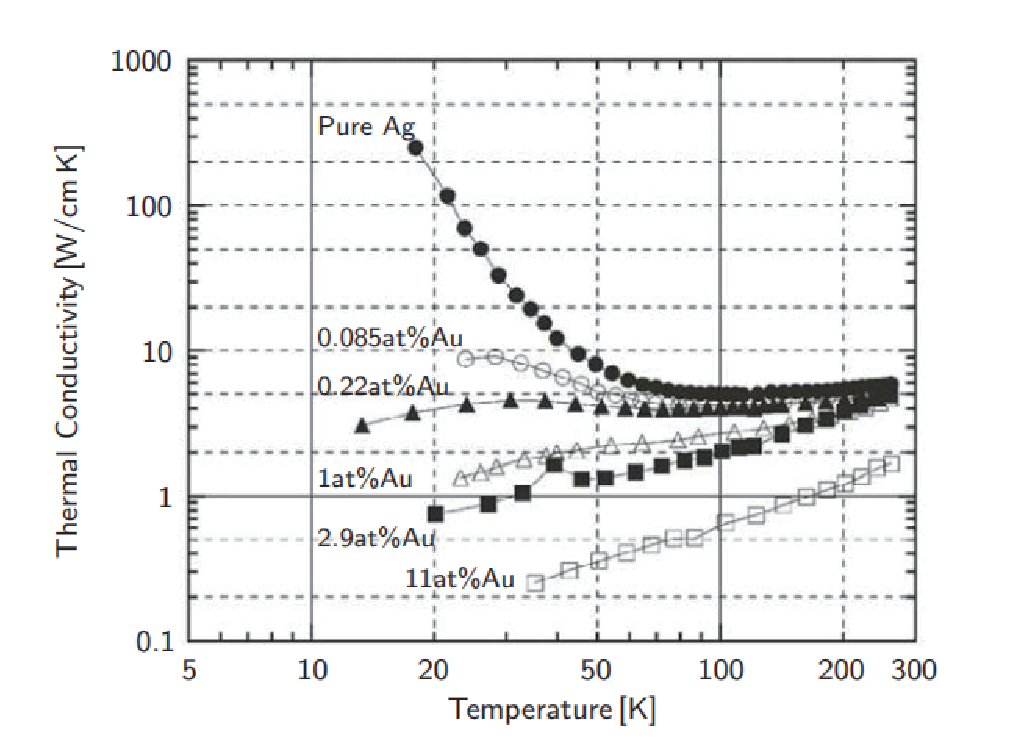
\includegraphics[scale=0.6]{chpt4/figs/fig4.23.eps}
	\caption{特定Ag-Cu合金的热导率随温度变化的数据。}
\end{figure}
\begin{figure}[htbp]
	\centering
	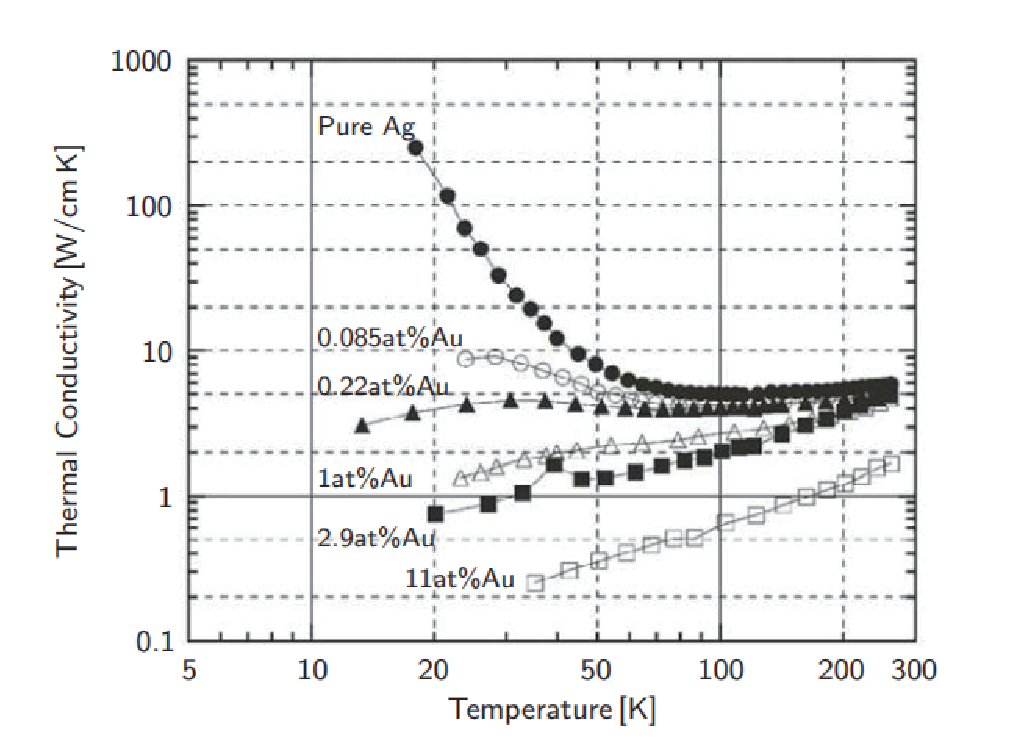
\includegraphics[scale=0.6]{chpt4/figs/fig4.23.eps}
	\caption{特定Ag-Cu合金的电导率随温度变化的数据。}
\end{figure}

\subsection{讨论4.16:FSV和CSV电流引线的保护}
因为FSV或CSV引线中的各HTS带 (问题4.5中的Bi2223/Ag-Au)都有较大的$i_c(T_\ell)$以及较小的$a_m$,
当进入正常态时,相比于可用的对流冷却能力来说,它产生的焦耳热耗散偏大:两种引线都不能承受哪怕短时
的流体阻塞。为了保护此类故障事件,引线必须并联常规金属带。这样,不仅减小了焦耳耗散,还提高了冷却表面积。

\textbf{FSV} 此时,FSV引线的$[Q_{in}]_{fs}$修改为$[Q_{in}]_{fs}^{n}$:
\begin{equation}% 4.75
[Q_{in}]_{fs}^{n}=\frac{[\tilde{kA}]_{fs}^{n}h_L}{\tilde{c}_p\ell}\ln\left[\frac{\tilde{c}_p(T_\ell-T_0)}{h_L}+1\right]
\end{equation}
式中,
\begin{equation}% 4.76
[\tilde{kA}]_{fs}^{n}=\tilde{k}[A_m]_{fs}+\tilde{k}[A_n]_{fs}
\end{equation}
$\~{k}_n$和$[A_n]_{fs}$分别是并联于HTS带的常规金属带的热导率和总截面积。
为了达到保护的目的,进入液氦的热输入增加了,如方程4.60指出的那样:$[Q_{in}]_{fs}^{n}>[Q_{in}]_{fs}$。方程4.59给出的$[\alpha]_{fs}$修改为:
\begin{equation}% 4.77a 4.77b
[\alpha_\ell]_{fs}^{n}=\frac{[\dot{m}_h]_{fs}^{n}\tilde{c}_p\ell}{\tilde{kA}_{fs}^{n}} 
=\ln\left[\frac{\tilde{c}_p(T_\ell-T_0)}{h_L}+1\right]
\end{equation}
式中,$[\dot{m}_h]_{fs}^{n}$是并联了常规金属带的FSV引线的氦气质量流量。
\begin{equation}% 4.74
[Q_\ell]_{cs}+Q_j-[Q_{in}]_{cs}=\dot{m}_h\tilde{c}_p(T_\ell-T_0)
\end{equation}

\textbf{CSV} 对于CSV引线,方程4.64给出的$[Q_{in}]_{cs}$修改为$[Q_{in}]_{cs}^{n}$:
\begin{equation}% 4.78
[Q_{in}]_{cs}^{n}=\frac{[\tilde{kA}]_{cs}^{n}h_L}{\tilde{c}_p\ell_{cs}}\ln\left[\frac{\tilde{c}_p(T_{cs}-T_0)}{h_L}+1\right]
\end{equation}
\begin{equation}% 4.79
[\tilde{kA}]_{cs}^{n}=\tilde{k}[A_m]_{cs}+\tilde{k}[A_n]_{cs}
\end{equation}
式中,$[A_n]_{cs}$是CSV引线中使用的常规金属带的总截面积。不论CSV引线是否并联常规金属带,
$\ell_{cs}$保持不变。另外,因为$[A_m]_{fs}$和$[A_m]_{cs}$不同,$[A_n]_{fs}$和$[A_n]_{cs}$可能不同。$[\alpha]_{cs}$也不同:
\begin{equation}% 4.80a 4.80b
[\alpha_\ell]_{cs}^{n}=\frac{[\dot{m}_h]_{cs}^{n}\tilde{c}_p\ell}{\tilde{kA}_{cs}^{n}} 
=\frac{1}{\xi_{cs}}\ln\left[\frac{\tilde{c}_p(T_{cs}-T_0)}{h_L}+1\right]
\end{equation}
式中,$[\dot{m}_h]_{cs}^{n}$是氦气质量流量;$\xi_{cs}(\ell_{c}/\ell)$是从$z = 0$处电流共享段
开始有并联常规金属带的无量纲长度。

对于CSV引线,$\beta_{cs}$还可以写为:
\begin{equation}% 4.81
\beta_{cs}^{n}=\sqrt{\frac{\tilde{\rho}_x\tilde{\rho}_nI_o(I_o-I_{c\ell})\ell^2}{[\tilde{kA}]_{cs}^{n}\tilde{\rho A}_{cs}^{n}(T_\ell-T_{cs})}-\frac{1}{4}([\alpha_\ell]_{cs}^{n})^2}
\end{equation}
式中,
\begin{equation}% 4.82
[\tilde{\rho A}]_{cs}^{n}=\tilde{\rho}_x[A_n]_{cs}+\tilde{\rho}_n[A_m]_{cs}
\end{equation}
方程4.71可以改写为下式:
\begin{align}% 4.83
\frac{1}{\xi_{cs}}\left[\frac{h_L}{\tilde{c}_p(T_\ell-T_{cs})}\right]&\ln\left[\frac{\tilde{c}_p(T_{cs}-T_0)}{h_L}+1\right]\left[\frac{\tilde{c}_p(T_{cs}-T_0)}{h_L}+1\right]^{\frac{1+\xi_{cs}}{2\xi_{cs}}}\\
&=\frac{\beta_{cs}^{n}}{\sin\beta_{cs}^{n}(1-\xi_{cs})}
\end{align}



\subsection{讨论4.17:HTS电流引线——有铜延伸}
因为所有的HTS电流引线,至少目前可用的,都仅在$T_\ell\sim$80 K以上可用。每一根HTS引线,无论
气冷与否,都必须连到常规金属引线上才能与室温端头连接。
对气冷HTS电流引线,优化的铜引线是理性的选择。
然而,正如前面提及的,同样的$I_o$下,4.2 K下任何HTS电流引线的$Q_in$都要小于优化的气冷铜引线。 
也就是说,HTS引线所用的氦流量对铜引线是不够用的。必须在铜引线的冷端引入额外的制冷工质(图4.21)。
这里,HTS段排出的氦气并不和引入到$\sim$80 K的制冷工质混合;它被转移走。 
大致说,新制冷工质有两个选择:1) 冷气体(氦或氮);2) 沸点为77.3 K的液氮。

\textbf{A. 制冷工质流量}

为了确定引入铜引线冷端的最小工质流量,我们这里分析一个$\sim$80 K–300 K温区内优化的气冷铜电流引线。
对一条载流为$I_o$、由质量流量$\dot{m}_{fl}$工质冷却的铜引线,铜电流引线上的一个微元的稳态 ($dT/dt=0$)功率方程($\zeta\equiv z/\ell_{cu}$):
\begin{equation}% 4.84
\frac{\tilde{k}_{cu}A_{cu}}{\ell_{cu}^{2}}\frac{d^2T}{d\zeta^2}-\frac{\dot{m}_{fl}\tilde{c}_{fl}}{\ell_{cu}}\frac{dT}{d\zeta}+\frac{T_{o}^{2}\gamma_{cu}}{A_{cu}}(T-T_o)+\frac{I_{o}^{2}\rho_o}{A_{cu}}=0
\end{equation}
方程4.84中,$\tilde{k}_{cu}$和$\tilde{c}_{fl}$分别是温度平均下的铜热导率和流体比热;
$\gamma_{cu}$和$\rho_o$分别是冷端温度$T_o$(这里是77 K)下的电阻温度系数和电阻率。
因为在区间77–293 K内,方程4.84的等号左侧最后一项相比第三项是可以忽略的,方程4.84可以简化为:
\begin{equation}% 4.85
\frac{d^2T}{d\zeta^2}-\left(\frac{\dot{m}_{fl}\tilde{c}_{fl}\ell_{cu}}{\tilde{k}_{cu}A_{cu}}\right)\frac{dT}{d\zeta}+\left(\frac{I_{o}^{2}\gamma_{cu}\ell_{cu}^{2}}{\tilde{k}_{cu}A_{cu}^{2}}\right)(T-T_o)=0
\end{equation}
代入$T(\zeta=1)\equiv T_{\ell_{cu}}, T(0)\equiv T_o$,以及$\theta(\zeta)\equiv T(\zeta)-T_o$,$\theta(\zeta)$可由下式给出:
\begin{equation}% 4.86
\theta(\zeta)=\frac{T_{\ell_{cu}}-T_o}{e^{\alpha_{cu}}\sin\beta_{cu}}e^{\alpha_{cu}\zeta}\sin\beta_{cu}\zeta
\end{equation}
式中,
\begin{equation}% 4.87a
\alpha_{cu}=\frac{\dot{m}_{fl}\tilde{c}_{fl}\ell_{cu}}{2\tilde{k}_{cu}A_{cu}}
\end{equation}
\begin{equation}% 4.87b 4.87c
\beta_{cu}=\sqrt{\frac{T_{o}^{2}\gamma_{cu}\ell_{cu}^{2}}{\tilde{k}_{cu}A_{cu}^{2}}-\left(\frac{\dot{m}_{fl}\tilde{c}_{fl}\ell_{cu}}{2\tilde{k}_{cu}A_{cu}}\right)^2}
=\sqrt{\frac{T_{o}^{2}\gamma_{cu}\ell_{cu}^{2}}{\tilde{k}_{cu}A_{cu}^{2}}-\alpha_{cu}^{2}}
\end{equation}

我们可以通过设置$d\theta/d\zeta|_{\zeta=1}=0$令$\theta_{mx}$出现在$\zeta=1$,得到:
\begin{equation}% 4.88a
\alpha_{cu}\sin\beta_{cu}+\beta_{cu}\cos\beta_{cu}=0
\end{equation}
\begin{equation}% 4.88b
\alpha_{cu}+\beta_{cu}\cot\beta_{cu}=0
\end{equation}
对于一组给定的引线参数,比如$A_{cu},\ell_{cu},I_o, \~{c}_{fl}, \gamma_{cu}$,有一组唯一的$\alpha_{cu}$和$\beta_{cu}$(进而,由方程4.87a和4.87b,可知$\.{m}_{fl}$的值)满足方程4.86。注意到$\cot\beta_{cu}$必须是负的,从而$\theta_{mx}$必须大于$\pi/2$,问题4.6D中还将看到。

\textbf{B. 冷端热输入和功率平衡}

冷端热输入$Q_o$为:
\begin{equation}% 4.89
Q_o=\frac{\tilde{k}_{cu}A_{cu}}{\ell_{cu}}\frac{d\theta(\zeta)}{d\zeta}\mid_0=\frac{\tilde{k}_{cu}A_{cu}\theta_{\ell_{cu}}\beta_{cu}}{\ell_{cu}e^{\alpha_{cu}}\sin\beta_{cu}}\simeq 0
\end{equation}

因为$e^{\alpha_{cu}}$很大,$Q_o\simeq 0$。这实际上就是问题4.6D中研究的6 kA铜引线的例子。

热端传导热$Q_{\ell_{cu}}$从定义上看是零(方程4.88a)。从而,由于引线两端既没有热输入也没有热流出,
制冷剂全部用于带走引线的焦耳热耗散$Q_j$:
\begin{equation}% 4.90
Q_j=\frac{I_{o}^{2}\gamma_{cu}}{A_{cu}}\int_{0}^{\ell_{cu}}\theta(z)dz 
=\frac{I_{o}^{2}\gamma_{cu}\ell_{cu}}{A_{cu}}\int_{0}^{1}\theta(\zeta)d\zeta
\end{equation}
联立方程4.86和4.90,代入方程4.87c,有:
\begin{align}% 4.91a
Q_j=&\frac{I_{o}^{2}\gamma_{cu}\ell_{cu}(T_{\ell_{cu}}-T_o)}{A_{cu}e^{\alpha_{cu}}\sin\beta_{cu}}\int_{0}^{1}e^{\alpha_{cu}\zeta}\sin\beta_{cu}\zeta d\zeta \\
=&\frac{I_{o}^{2}\gamma_{cu}\ell_{cu}(T_{\ell_{cu}}-T_o)}{A_{cu}(\alpha_{cu}^{2}+\beta_{cu}^{2})}(\alpha_{cu}-\beta_{cu}\cot\beta_{cu}) \\
&+(terms containing e^{-\alpha_{cu}}) \\
\simeq&\frac{\tilde{k}_{cu}A_{cu}}{\ell_{cu}}(T_{\ell_{cu}}-T_o)(\alpha_{cu}-\beta_{cu}\cot\beta_{cu})
\end{align}
代入方程4.88b,方程4.91a成为:
\begin{equation}% 4.91b
Q_j=\frac{\tilde{k}_{cu}A_{cu}}{\ell_{cu}}(T_{\ell_{cu}}-T_o)(\alpha_{cu}+\alpha_{cu})
\end{equation}
接下来,与方程4.87a联立,方程4.91b成为:
\begin{equation}% 4.92
Q_j=\dot{m}_{fl}\tilde{c}_{fl}(T_{\ell_{cu}}-T_o)
\end{equation}
方程4.92表明,铜引线在整个长度上产生的焦耳热耗散被引线冷端引入的液体冷却功率平衡。

\textbf{C. 液氮质量流量}

当77 K液氮被以质量流量$\.{m}_{fl}$引入到引线冷端,它在冷端产生的冷却功率为
$Q_{n2}=\.{m}_{fl}h_{n2}$,其中$h_{n2}$=199 J/g是液氮在77 K的汽化潜热

当气冷铜引线运行于液氦环境中时,$Q_in$由$\.{m}_h h_L$匹配,其中$h_L$ = 20.7 J/g是氦的汽化热;
氦气的$\.{m}_h$足以保持整个引线的稳定。如前所述,因为液氮的冷却功率$Q_o\simeq 0$,$\.{m}_{fl}h_{n2}$无法在冷端匹配。实际发生的是$\.{m}_{fl}h_{n2}$吸收铜引线底端部分
(从冷端到$\ell_{\ell_q}$)产生的焦耳热耗散。也就是说,冷端的77 K锚点从$z=0$延伸到了$z=q$。
由于引线使电阻性的,这个77 K的延伸段产生焦耳耗散$Q_{j_{\ell q}}$,由$\.{m}_{fl}h_{n2}$匹配。
注意到方程4.84等号左侧的最后一项在4.85中是忽略掉的,而在77 K情况下是不能忽略的。我们有:
\begin{equation}% 4.93
Q_{j_{\ell q}}=\frac{\rho_oI_{o}^{2}\ell_{\ell q}}{A_{cu}}=\dot{m}_{fl}h_{n2}
\end{equation}
方程4.93中,$\ell_{\ell_q}$和$\.{m}_{fl}$还不知道。

考虑引线底端位于77 K的部分 ($z=\ell_{\ell_q}$长),引线的有效气冷长度缩短为($\ell_{cu}-\ell_{\ell_q}$,方程4.88b于是成为:
\begin{equation}% 4.94
\alpha_{cu}^{\prime}+\beta_{cu}^{\prime}\cot\beta_{cu}^{\prime}=0
\end{equation}
式中,
\begin{equation}% 4.95a
\alpha_{cu}^{\prime}=\frac{\dot{m}_{fl}\tilde{c}_{fl}(\ell_{cu}-\ell_{\ell q})}{2\tilde{k}_{cu}A_{cu}}
\end{equation}
\begin{equation}% 4.95b
\beta_{cu}^{\prime}=\sqrt{\frac{I_{o}^{2}\gamma_{cu}(\ell_{cu}-\ell_{\ell q})^2}{\tilde{k}_{cu}A_{cu}^{2}}-(\alpha_{cu}^{\prime})^2}
\end{equation}
满足方程4.93和4.94的$\.{m}_{fl}$和$\ell_{\ell_q}$组是惟一的。

\subsection{问题4.6:6 kA气冷HTS电流引线}
问题4.6将问题4.4和4.5中讨论的设计概念应用于三种6 kA的气冷HTS引线:
A) FSV,无并联常规金属带;B) FSV,有120根并联常规金属带;
C) CSV,有相同根数的常规金属带。
表4.12给出Bi2223/Ag-Au带的关键参数。表中,$a_m$是单带Ag-Au基底的截面积:
也即 $[A_m]_{fs}=N_{fs} a_m; I_c(T)=N_{fs} i_c(T_\ell);I_c(T_0)=N_{fs}i_c(T_0)$。
我们假定,各带的全部有效长度都置于0.2 T的垂直场中。$\~{k}$和$\~{\rho}_x$分别是Ag-Au
在表4.12中所给的温度区间的平均热导率和平均电导率。
表4.13给出了紫铜带的关键参数。

\subsubsection{问题4.6A:FSV,无并联常规金属带}

a) 证明这根6 kA的气冷FSV引线,$N_{fs}$=75。

b) 证明若这根引线$\ell$=20 cm,有$[Q_{in}]_{fs}$ =0.0786 W。这里,$\ell$在一端
必须足够“长”以确保与气体有良好的热交换,另一端足够“短”以限制Bi2223/Ag-Au带材的费用。

c) 验证方程4.61通过计算各功率项,可用于这根引线。

\colorbox{red}{表4.12和4.13}

\subsubsection{问题4.6A之解}

a) 因为$I_o=N_{fs} i_c(T_\ell)$,我们有:$N_{fs}$=6,000 A/80 A=75。

b) 将$\tilde{k}$ = 0.327 W/cmK; $[A_m]_{fs}=N_{fs} a_m= 0.416\ \mathrm{cm^2}$; $h_L$ = 20.7 J/g; $\~{c}_p$=5.28 J/gK (4.2 K和77 K间的平均值) ; $T_\ell$= 77.3K; $T_0$ = 4.2 K, 以及$\ell$=20 cm代入方程4.60,有:
\begin{align*}% 4.60
[Q_{in}]_{fs}=&\frac{\tilde{k}[A_m]_{fs}h_L}{\tilde{c}_p\ell}\ln\left[\frac{\tilde{c}_p(T_\ell-T_0)}{h_L}+1\right] \\\tag{4.60}
=&\frac{(0.327\ \mathrm{W/cmK})(0.461\ \mathrm{cm^2})(20.7\ \mathrm{J/g})}{(5.28\ \mathrm{J/gK})(20\ \mathrm{cm})} \\
&\times\ln\left[\frac{(5.28\ \mathrm{J/gK})(77.3\ \mathrm{K}-4.2\ \mathrm{K})}{(20.4\ \mathrm{J/g})}+1\right] \\
=&0.0798\ \mathrm{W}
\end{align*}

讨论4.14A (方程4.32b )已经研究,对气冷铜制6 kA引线,有$Q_{in}\simeq$6 W;于是,
$\sim$0.08 W实质上是一个很客观的提升。

c) 由$[Q_{in}]_{fs}$ = 0.0798 W,我们有
$\dot{m}_h]_{fs}= [Q_{in}]_{fs}/h_L$ = 0.00385 g/s。在$z=\ell$处的热输入由方程S4.5b的第一种形式给出:
\begin{align*}
[Q_\ell]_{fs}&=[\dot{m}_h]_{fs}h_L\left[\frac{\tilde{c}_p(T_\ell-T_0)}{h_L}+1\right] \\
&=(0.00385\ \mathrm{g/s})(20.7\ \mathrm{J/g})\left[\frac{(5.28\ \mathrm{J/gK})(77.3\ \mathrm{K}-4.2\ \mathrm{K})}{(20.7\ \mathrm{J/g})}+1\right] \\
&=1.556\ \mathrm{W}
\end{align*}
于是,$[Q_\ell]_{fs}−[Q_{in}]_{fs}$=1.486 W,基本上等于$[\dot{m}_h]_{fs} \tilde{c}_p(T_\ell-T_0)$=1.487 W.

\subsubsection{问题4.6B:FSV,有并联常规金属带}
这里,我们研究一条并联120根常规金属带的FSV引线,类似于问题4.6A中的引线,
$[A_n]_{fs}$=1.735 $cm^2$ (表4.13)。
尽管未经证明,截面为1.735 $cm^2$的常规导体足以抵抗典型操作条件下可能发生的
流体阻塞故障。

a) 使用方程4.75,计算$[Q_{in}]_{fs}^n$。因为存在常规金属,$[A_n]_{fs}\gg [A_m]_{fs}$,
$[Q_{in}]_{fs}^n\gg[Q_{in}]_{fs}$=0.0798 W。

b) 数值验证功率项在这条引线上也是平衡的。

\subsubsection{问题4.6B之解}
a) 首先,我们使用方程4.76计算$[\tilde{kA}]_{fs}^{n}$。注意$[A_m]_{fs}=0.416\ \mathrm{cm^2}$:
\begin{align*}
[\tilde{kA}]_{fs}^{n}=&(0.327\ \mathrm{W/cm K})(0.416\ \mathrm{cm^2})+(0.350\ \mathrm{W/cmK})(1.735\ \mathrm{cm^2}) \\
=&0.136\ \mathrm{W cm/K}+0.607\ \mathrm{W cm/K}=0.743\ \mathrm{W cm/K}
\end{align*}
根据方程4.75,我们有:
\begin{align}% 4.75
[Q_{in}]_{fs}^{n}=&\frac{\tilde{kA}_{fs}^{n}h_L}{\tilde{c}_p\ell}\ln\left[\frac{\tilde{c}_p(T_\ell-T_0)}{h_L}+1\right] \\
=&\frac{(0.743\ \mathrm{W cm/K})(20.7\ \mathrm{J/g})}{(5.28\ \mathrm{J/gK})(20\ \mathrm{cm})} \\
&\times\ln\left[\frac{(5.28\ \mathrm{J/gk})(77.3\ \mathrm{K}-4.2\ \mathrm{K})}{(20.7\ \mathrm{J/g})}+1\right]=0.4337\ \mathrm{W}
\end{align}

注意到尽管实际上$[Q_{in}]_{fs}^n\gg[Q_{in}]_{fs}$,0.4337 W仍然仅为相应的铜引线
($\sim$6 W)的$\sim$1/14。同时,根据方程4.35b,一条优化的气冷引线,额定电流6 kA,
有效长度($\ell$)20 cm,截面为$A = 0.480\ \mathrm{cm^2}$,
约为$[A_n]_{fs}$ = 1.735$\ \mathrm{cm^2}$的30\%。
尽管$[A_n]_{fs}$很大,$[Q_{in}]_{fs}^n$仍为$Q_{I_o}$的$\sim$ 1/14。这主要是因为
$\~{k}_n\ll k_0$,其中$k_0$是铜在4.2 K附近的热导率,
即0.350 W/cmK ($\~{k}_n$) vs. 6 W/cmK ($k_0$)。同时注意到,在引线的这个部分($\ell$),
没有焦耳热产生。

b) 代入$[Q_{in}]_{fs}^n$= 0.4337W,我们得到$\dot{m}_h]_{fs}^{n}= [Q_{in}]^n_{fs}/h_L\simeq$
0.021 g/s。在$z=\ell$处的热输入$[Q_\ell]_{fs}^{n}$,尽管未推导,但类似于方程S4.5b。于是:
\begin{align*}
[Q_\ell]_{fs}^{n}&=[\dot{m}_h]_{fs}^{n}h_L\left[\frac{\tilde{c}_p(T_\ell-T_0)}{h_L}+1\right] \\
&\simeq(0.021\ \mathrm{g/s})(20.7\ \mathrm{J/g})\left[\frac{(5.28\ \mathrm{J/gk})(77.3\ \mathrm{K}-4.2\ \mathrm{K})}{(20.7\ \mathrm{J/g})}+1\right]\\
&=8.540\ \mathrm{W}
\end{align*}
于是,我们有:

$[Q_\ell]_{fs}^{n}-[Q_{in}]_{fs}^{n}=8.106\ \mathrm{W}\simeq [\.{m}_h]_{fs}^n \~{c}_p(T_\ell-T_0)$=8.105 W。


\subsubsection{问题4.6C:CSV,有并联常规金属带}
这里,我们考虑一根CSV引线,其参数为$N_{cs} = (2/3)N_{fs}$ = 50。类似于上面研究的
FSV引线,增加了同样数量(120)跟常规金属带。

a) 证明这根CSV引线的$T_{cs}$ = 69.3K。假设$i_c(T)$是$T$的线性函数,且有$i_c(T_0)$=445.5 A,$i_c(T-\ell)$=80 A,如表4.12所给。

b) 对$\ell$=20 cm (与FSV情况同),确定如下CSV简单特例的$\xi_{cs}$:
\begin{subequations}% 4.96a
	\begin{align*}
\sin\beta_{cs}^{n}(1-\xi)&=1\\
\beta_{cs}^{n}(1-\xi_{cs})&=\pi/2
	\end{align*}
\end{subequations}

你可以迭代的确定$\xi_{cs}$。首先,猜一个$\xi_{cs}$值,根据方程4.96b计算$\beta_{cs}^n$,
将$\xi_{cs}$和$\beta_{cs}^n$代入方程4.83,检查其是否已经满足。
因为假定了$i_c(T)$是$T$的线性函数,$\xi_{cs}$的一个合适的起始值可选0.9($\simeq $69.3/77.3)。

c) 验证b)中得到的$\beta_{cs}^n$与方程4.81计算得到的$\beta_{cs}^n$是一致的。 

d) 使用方程4.78,计算$z=0$处输入液氦的热量$[Q_{in}]^n_{cs}$。

e) 数值计算下面功率平衡方程中的每一项,证明功率是平衡的。
\begin{equation}% 4.97
[Q_\ell]_{cs}^{n}+[Q_j]_{cs}^{n}-[Q_{in}]_{cs}^{n}=[\dot{m}_h]_{cs}^{n}\tilde{c}_p(T_\ell-T_0)
\end{equation}
$[Q_\ell]_{cs}^{n}$是引线$z=\ell$处的热输入;$[Q_j]_{cs}^{n}$是电流分享区内的焦耳热耗散;
$[Q_{\ell_{cs}}]_{cs}$是引线$z=\ell_{cs}$处的热输出。
$[Q_\ell]_{cs}^{n}$和$[Q_j]_{cs}^{n}$由方程S5.9和S5.14的变种给出:
\begin{equation}% 4.98
[Q_\ell]_{cs}^{n}=\frac{[\tilde{kA}]_{cs}^{n}(T_\ell-T_{cs})}{\ell}[\frac{1}{2}[\alpha_\ell]_{cs}^{n}+\beta_{cs}^{n}\cot\beta_{cs}^{n}(1-\xi_{cs})]
\end{equation}

\begin{equation}% 4.99
[Q_j]_{cs}^{n}=\frac{[\tilde{kA}]_{cs}^{n}(T_\ell-T_{cs})}{\ell}\left[\frac{1}{2}[\alpha_\ell]_{cs}^{n}+\beta_{cs}^{n}\cot\beta_{cs}^{n}(1-\xi_{cs}) 
+\beta_{cs}^{n}\frac{e^{\frac{[\alpha_\ell]_{cs}^{n}\xi_{cs}}{2}}}{e^{\frac{[\alpha_\ell]_{cs}^{n}}{2}}\sin\beta_{cs}^{n}(1-\xi_{cs})}\right]
\end{equation}
因为这里$\beta_{cs}^n (1-\xi_{cs})=\pi/2$,方程4.98和4.99简化为:
\begin{equation}% 4.100
[Q_\ell]_{cs}^{n}=\frac{[\tilde{kA}]_{cs}^{n}(T_\ell-T_{cs})}{\ell}\times\frac{1}{2}[\alpha_\ell]_{cs}^{n}
\end{equation}

\begin{equation}% 4.101
[Q_j]_{cs}^{n}=\frac{[\tilde{kA}]_{cs}^{n}(T_\ell-T_{cs})}{\ell}\left[\frac{1}{2}[\alpha_\ell]_{cs}^{n}+\beta_{cs}^{n}e^{\frac{[\alpha_\ell]_{cs}^{n}(\xi_{cs}-1)}{2}}\right]
\end{equation}

\subsubsection{问题4.6C之解}
a) 因为$I_c(T_\ell)=N_{cs}i_c(T_\ell)$,其中$N_{cs}$=50,由表4.12,$i_c(T_\ell)$=80 A,在$T=$77.3 K时,我们有:$I_c(T_\ell)= 50\times 80= 4,000$ A;类似的,在
$T_0$=4.2 K时有$I_c(T_0)$ = 22,275 A。
于是,这种参数的Bi2223/Ag-Au带在77.3 K和4.2 K之间的$I_c(T)$满足:
\begin{equation}
 I_c(T)=23,325-250T[\ \mathrm{A}]
\end{equation}
式中,$T$是开氏温度。这个方程给出$T_c$=93.3 K。由方程S6C.1,我们可以解出$I_c(T_{cs})$=6000 A下的
$T_{cs}$=69.3 K。

b) 如表4.14给出的,$\xi_{cs}$=0.94505,它给出$\beta_{cs}^n$=28.586。

c) $[A_m]_{cs}=N_{cs} a_m=50\times 0.555\ \mathrm{mm^2}=0.2775\ \mathrm{cm^2}$(表4.12);
$[A_n]_{cs}=[A_n]_{fs}=1.735\ \mathrm{cm^2}$(表4.13)。于是:
\begin{align*}% 4.79
[\tilde{kA}]_{cs}^{n}&=\tilde{k}[A_m]_{cs}+\tilde{k}[A_n]_{cs} \\
&=(0.327\ \mathrm{W/cmK})(0.2775\ \mathrm{cm^2})+(0.350\ \mathrm{W/cmK})(1.735\ \mathrm{cm^2}) \\
&=0.0907\ \mathrm{W cm/K}+0.607\ \mathrm{W cm/K}=0.698\ \mathrm{W cm/K} \tag{4.79}
\end{align*}

\begin{align*}% 4.82
[\tilde{\rho A}]_{cs}^{n}&=\tilde{\rho}_x[A_m]_{cs}+\tilde{\rho}_n[A_n]_{cs} \\
&=(1\mu\Omega\ \mathrm{cm})(1.735\ \mathrm{cm^2})+(2.25\mu\Omega\ \mathrm{cm})(0.2775\ \mathrm{cm^2}) \\
&=1.735\mu\Omega\ \mathrm{cm^3}+0.624\mu\Omega\ \mathrm{cm^3}=2.359\mu\Omega\ \mathrm{cm^3} \tag{4.82}
\end{align*}

\begin{align*}% 4.80b
[\alpha_\ell]_{cs}^{n}&=\frac{1}{\xi_{cs}^{n}}\ln\left[\frac{\tilde{c}_p(T_{cs}-Y_0)}{h_L}+1\right] \\
&=\frac{1}{0.94505}\ln\left[\frac{(5.28\ \mathrm{J/gK})(69.3\ \mathrm{K}-4.2\ \mathrm{K})}{(20.7\ \mathrm{J/g})}+1\right] \\
&=\frac{1}{0.94505}\ln(17.605)=3.035 \tag{4.80b}
\end{align*}
于是,通过计算4.81,得到$([\alpha_\ell]_{cs}^2/4$:
\begin{align*}
\frac{1}{4}([\alpha_\ell]_{cs}^{n})^2=2.303
\end{align*}

\colorbox{red}{表4.14}

将必要的值代入方程4.81,得到:
\begin{align*}% 4.81
\beta_{cs}^{n}&=\sqrt{\frac{\tilde{\rho}_x\tilde{\rho}_nI_o(I_o-I_{c\ell})\ell^2}{[\tilde{kA}]_{cs}^{n}[\tilde{\rho A}]_{cs}^{n}(T_\ell-T_{cs})}-\frac{1}{4}([\alpha_\ell]_{cs}^{n})^2}
28.586\\ \tag{4.81}
&=\sqrt{\frac{(1\mu\Omega\ \mathrm{cm})(2.25\mu\Omega\ \mathrm{cm})(6\ \mathrm{kA})(6\ \mathrm{kA}-4\ \mathrm{kA})(20\ \mathrm{cm})^2}{(0.698\ \mathrm{W cm/K})(2.359\mu\Omega\ \mathrm{cm^3})(77.3\ \mathrm{K}-69.3\ \mathrm{K})}-2.303}
28.586\\
&\simeq\sqrt{817.58}=28.593
\end{align*}

d) 由$\xi_{cs}=0.94505$和$\ell=20$ cm,得$\ell_{cs}$=18.9 cm。于是,这条CSV引线的电流共享段
长为1.1 cm,从$z$=18.9 cm到$z$=20 cm。由方程4.78:
\begin{align*}% 4.78
[Q_{in}]_{cs}^{n}&=\frac{\tilde{kA}_{cs}^{n}h_L}{\tilde{c}_p\ell_{cs}}\ln\left[\frac{\tilde{c}_p(T_{cs}-T_0)}{h_L}+1\right] \\ \tag{4.78}
&=\frac{(0.698\ \mathrm{W cm/K})(20.7\ \mathrm{J/g})}{(5.28\ \mathrm{J/gK})(18.9\ \mathrm{cm})}\ln\left[\frac{(5.28\ \mathrm{J/gK})(69.3\ \mathrm{K}-4.2\ \mathrm{K})}{(20.7\ \mathrm{J/g})}+1\right] \\
&=(0.1448\ \mathrm{W})(2.868)=0.4153\ \mathrm{W}
\end{align*}
于是,如我们所预料的,$[Q_{in}]_{cs}^n$=0.4153 W$<[Q_{in}]_{fs}^n$=0.4296 W;
$[Q_{in}]_{cs}^n$约为铜的1/15。由$[Q_{in}]_{cs}^n$=0.4153 W,可得$[\.{m}_h]_{cs}^n$=0.02006 g/s。

e) 应用方程4.100和4.101,我们有:
\begin{align*}% 4.100
[Q_\ell]_{cs}^{n}&=\frac{[\tilde{kA}]_{cs}^{n}(T_\ell-T_{cs})}{\ell}\left(\frac{[\alpha_\ell]_{cs}^{n}}{2}\right) \\ \tag{4.100}
&=\frac{(0.698\ \mathrm{W cm/K})(77.3\ \mathrm{K}-69.3\ \mathrm{K})}{(20\ \mathrm{cm})}\left(\frac{3.035}{2}\right)\\
&=0.4237\ \mathrm{W}
\end{align*}
\begin{align*}% 4.101
[Q_j]_{cs}^{n}&=\frac{[\tilde{kA}]_{cs}^{n}(T_\ell-T_{cs})}{\ell}\left[\frac{[\alpha_\ell]_{cs}^{n}}{2}+\beta_{cs}^{n}+\beta_{cs}^{n}e^{\frac{[\alpha_\ell]_{cs}^{n}(\xi_{cs}-1)}{2}}\right] \\\tag{4.101}
&=\frac{[\tilde{kA}]_{cs}^{n}(T_\ell-T_{cs})}{\ell}\left[\left(\frac{3.035}{2}\right)+(28.586)e^{\frac{3.035(0.645-1)}{2}}\right] \\
&=\frac{(0.698\ \mathrm{W cm/K})(77.3\ \mathrm{K}-69.3\ \mathrm{K})}{(20\ \mathrm{cm})}\left[\left(\frac{3.035}{2}\right)+26.30\right]=7.7743\ \mathrm{W}
\end{align*}
由$[\dot{m}_h]_{cs}^{n}\tilde{c}_p(T_\ell-T_0)$=(0.02006 g/s)(5.28 J/gK)(77.3 K-4.2 K)=7.7743 W
和$[Q_{in}]_{cs}^{n}=$0.4153 W,我们可以得到:
\begin{align*}% 4.97
[Q_\ell]_{cs}^{n}+[Q_j]_{cs}^{n}-[Q_{in}]_{cs}^{n}&=[\dot{m}_h]_{cs}^{n}\tilde{c}_p(T_\ell-T_0)\\\tag{4.97}
0.4237\ \mathrm{W}+7.7658-0.4153=7.7742\ \mathrm{W} \\
&\simeq 7.7743\ \mathrm{W}             
\end{align*}


\subsection{讨论4.18:“最优”CSV引线}
如我们在问题4.6C中所见,最大的功率项是$[Q_j]_{cs}^n$=7.7659 W,而$[Q_{in}]_{cs}^n$=0.4153 W
是和FSV的$[Q_{in}]_{fs}^n$=0.4337 W是非常接近的。

于是,由于$[Q_j]_{cs}^n$值很大,CSV引线的$[Q_{in}]_{cs}^n$可以和$[Q_{in}]_{fs}^n$具有可比性的
唯一方法是$[Q_{\ell}]_{cs}^n\ll [Q_{\ell}]_{fs}^n$。这其实恰好就是问题4.6B中b)以及问题4.6C中e)的解中所看到的:$[Q_{\ell}]_{fs}^n$=8.540 W,$[Q_{\ell}]_{cs}^n$=0.4237 W。这是怎么回事?答案可以从方程4.98中看到:
\begin{equation*}% 4.98
[Q_\ell]_{cs}^{n}=\frac{[\tilde{kA}]_{cs}^{n}(T_\ell-T_{cs})}{\ell}\left[\frac{1}{2}[\alpha_\ell]_{cs}^{n}+\beta_{cs}^{n}\cot\beta_{cs}^{n}(1-\xi_{cs})\right]
\end{equation*}
通过选择方程等号右侧中括号项内合适的$\beta_{cs}^n$和$\xi_{cs}$,可以令$[Q_\ell]_{cs}^{n}=0$。
对于$\beta_{cs}^{n}(1-\xi_{cs})>\pi/2$,$\cot\beta_{cs}^{n}(1-\xi_{cs})<0$,确实存在一组
$\beta_{cs}^n$和$\xi_{cs}$不仅令$[Q_\ell]_{cs}^{n}=0$,还满足方程4.83。这样的一组值实质上最小化了
$[Q_{in}]_{cs}^n$,给出了一条可满足保护条件的带有常规金属的“优化”CSV引线。

\subsubsection{问题4.6D:铜段($\sim$80 K-300 K)}
这里我们研究6 kA气冷电流引线,或如问题4.6B耦合于FSV引线,或如问题4.6C耦合于CSV引线。
我们将确定三种流量的值:1) 气氦; 2) 气氮;3) 液氮。
对液氮的情况,我们还将确定$\ell_{\ell_q}$的值。表4.15列出了6 kA气冷铜引线的关键参数值。
冷端($z=0$)位于77.3 K,热端($z=\ell_{cu}$)位于293 K。

a) 当进入77. K冷端点($z$=0)的制冷工质是气氦时,确定$\.{m}_{fl}$。

b) 如方程4.89中讨论的,证明冷端的热传导输入$Q_o$实际是小的可以忽略。

c) 当进入77. K冷端点($z$=0)的制冷工质是气氮时,确定$\.{m}_{fl}$。

d) 当进入77. K冷端点($z$=0)的制冷工质是液氮时,确定$\.{m}_{fl}$,同时确定$\ell_{\ell_q}$。

\colorbox{red}{Biao 4.15}

\subsubsection{问题4.6D之解}
a) 将表4.15中的参数值代入方程4.87c,我们有:
\begin{align*}
\beta_{cu}=\sqrt{\frac{I_{o}^{2}\gamma_{cu}\ell_{cu}^{2}}{\tilde{k}_{cu}A_{cu}^{2}}-\alpha_{cu}^{2}}&=\sqrt{\frac{(6\ \mathrm{kA})^2(7.01\ \mathrm{n\Omega cm/K})(38\ \mathrm{cm})^2}{(4\ \mathrm{W /cmK})(1.19\ \mathrm{cm^2})^2}-\alpha_{cu}^{2}} \\
&=\sqrt{64.333-\alpha_{cu}^{2}} \tag{S6D.1}
\end{align*}
存在一组$\beta_{cu}$和$\alpha_{cu}$同时满足方程4.88b和S6.D.1。这两个方程可以迭代求解;
表4.16给出了迭代结果。从表4.16,我们看到$\beta_{cu}=2.786750\simeq 2.786885$,于是
$\alpha_{cu}=7.521055$。从方程4.87a,解出$\.{m}_{fl}$:
\begin{align*}
\dot{m}_{fl}=\frac{2\alpha_{cu}\tilde{k}_{cu}A_{cu}}{\tilde{c}_{fl}\ell_{cu}} 
=\frac{2(7.521)(4\ \mathrm{W/cmK})(1.19\ \mathrm{cm^2})}{(5.28\ \mathrm{J/gK})(38\ \mathrm{cm})}=0.357\ \mathrm{g/s} \tag{S6D.2}
\end{align*}
这里算得的氦质量流量0.357 g/s非常接近于AMI 6 kA气冷铜引线的蒸发液氦质量流量$\.{m}_h$,即
$Q_{in}\sim$7.2 W:$\.{m}_h\sim$0.35 g/s($\sim$7.2 W/20.4 J/g)。77.3 K和293 K间
的总冷却功率由$\dot{m}_{fl}\tilde{c}_{fl}(T_{\ell_{cu}}-T_o)$给出,为407 W。

b) 代入$e^{\alpha_{cu}}=1846$,$\sin(159.669^\circ)$=0.3474,$\theta_{\ell_{cu}}$=216 K,以及
其他参数到方程4.89,有:
\begin{align*}% 4.89
Q_o&=\frac{\tilde{k}_{cu}A_{cu}}{\ell_{cu}}\frac{d\theta(\zeta)}{d\zeta}\mid_0=\frac{\tilde{k}_{cu}A_{cu}\theta_{\ell_{cu}}\beta_{cu}}{\ell_{cu}e^{\alpha_{cu}}\sin\beta_{cu}}\simeq 0 \\ \tag{4.89}
&=\frac{(4\ \mathrm{W/cmK})(1.19\ \mathrm{cm^2})(216\ \mathrm{K})(2.787)}{(38\ \mathrm{cm})(1846)(0.3474)}\\
&\simeq 0.118\ \mathrm{W}\simeq 0
\end{align*}

c) 在a)中确定的$\beta_{cu}$和$\alpha_{cu}$同样适用于气氮情况。两者唯一的不同是比热:气氮的是1.04 J/gK。于是:$\dot{m}_{fl}$=1.812 g/s。

\colorbox{red}{表4.16}


d) 这里我们来确定满足方程4.93、4.94和4.95在给定参数值$\rho_o, \gamma_{cu}, I_o, \~{k}_{cu}, A_{cu}$下的$\ell_{\ell_q}$。用迭代的方法确定$\ell_{\ell_q}$是最简单的。我们进行如下步骤:

步骤1:猜$\ell_{\ell_q}$(表4.17的第一列);

步骤2:从方程4.93计算$\dot{m}_{fl}$(第二列);

步骤3:将$\ell_{\ell_q}$和$\dot{m}_{fl}$代入方程4.95a,计算$\alpha_{cu}^\prime$(第三列);

步骤4:将$\alpha_{cu}^\prime$代入方程4.95b,计算$\beta_{cu}^\prime$(第四列);

步骤5:用角度制表示$\beta_{cu}^\prime$(第五列):它必须在90到180之间;

步骤6:计算$\cot\beta_{cu}^\prime$(第六列);

步骤7:使用方程4.94计算$\alpha_{cu}^\prime$(第七列)。

如果步骤7计算的$\alpha_{cu}^\prime$与步骤3计算值基本相等,迭代完成;迭代开始猜的$\ell_{\ell_q}$是正确的。表4.17给出了上述迭代的结果,$\ell_{\ell_q}$=26.98 cm($\simeq$27 cm)和$\dot{m}_{fl}$=0.902 g/s是希望得到的值。

于是,铜引线的底端有了液氮,具体说是有总长$\simeq$27 cm浸入液氮和气氮混合物中,这一段的温度是77.3 K。仅其余部分,从$z\simeq$27 cm到$z$=38 cm是由气氮流冷却的;它的温度从$z\simeq$27 cm 的77.3K升高
到$z=$38 cm的293 K。 

与c)中77.3 K气氮的$\dot{m}_{fl}$=1.812 g/s相比,液氮流量仅需一半。这是因为液氮在77.3 K汽化时可吸收大量热量,即199 J/g,相等于气氮温升将近200 K($\tilde{c}_{fl}=1.04 J/gK$)。
如果引入到铜引线的制冷工质为77.3 K的氮,c)和d)的结果表明77.3 K的液氮更好。

\colorbox{red}{表4.17}

\subsection{问题4.7:气冷铜电流引线}
Vapor-cooled current leads for a superconducting magnet operated in a bath of liquid
helium may be entirely of copper (DISCUSSION 4.14) or superconducting over
the lower cold section (PROBLEMS 4.4–4.6), extended to the room-temperature
terminal by a copper lead rated at the same current.

In some applications, current leads carry a rated current only occasionally or even
rarely during the life of a magnet [4.81–4.84]. Examples of occasional use include
magnets of low duty cycle in which the magnets are energized periodically, each
time for a short duration. When the total duration of “off-current” operation far
exceeds that of “on-current” operation, it may be possible to reduce the long-term
consumption of helium with vapor-cooled leads having a $Q_0/Q_{I_o}$ratio (Eq. 4.42)
significantly smaller than the ∼0.6 achievable with copper leads.

Because$Q_0\propto \~{k}$(Eq. 4.40), such low-Q0 leads should be of an alloy (e.g., brass),
rather than pure copper. It necessarily implies that such an alloy lead would have
Joule dissipation rate greater than its copper counterpart. Because the effluent
helium flow rate would remain roughly the same, to be effective, the alloy lead
must operate in overcurrent mode, and the thermal behavior of such a lead in
overcurrent mode becomes an important design and operation issue [4.85].

对下面的问题,铜的物性按如下取值:热导率$[k_0]_{br}$=22 W/mK,电阻率$[\rho_0]_{br}=21\ \mathrm{n\Omega m}$,上述两者都是在$T_0$时的值。另有$\int_{T_0}^{T_\ell}dT/\rho_{br}(T)$=
0.97$\times 10^{10} K/\Omega m$[4.86]。

a) 证明黄铜引线的$I_o\ell/A$为(紫铜近似为$2.3\times 10^7$A/m):
\begin{equation}% 4.102
\left[\frac{I_o\ell}{A}\right]_{br}\equiv[\zeta_o]_{br}\simeq0.35\times 10^7\ \mathrm{A/m}
\end{equation}
也即,具有相同$\ell$和$A$的黄铜引线,其优化额定电流仅为紫铜的$\sim 1/7$。

b) 证明冷端热输入和额定电流之比$[Q_{I_o}/I_o]$由下式给出:
\begin{equation}% 4.103
\left[\frac{Q_{I_o}}{I_o}\right]_{br}\simeq 1.25\ \mathrm{mW/A}
\end{equation}
紫铜的这个比值是0.77 mW/A(方程4.32b)。对黄铜引线,尽管电阻率更大,是紫铜在4.2 K时的约100倍,但
$[Q_{I_o}/I_o]$仅为比紫铜大约60\%。

c) 证明无电流时冷端热输入和引线电流之比$[Q_0/I_o]$由下式给出:
\begin{equation}% 4.104
\left[\frac{Q_0}{Q_{I_o}}\right]_{br}\simeq 0.21
\end{equation}
计算中,使用$\~{k}_{br}$=55 W/mK(表4.18);$\~{c}_p$=5.2 kJ/kgK;$c_{p0}$=6.0 kJ/kgK。

\textbf{过流模式}

As stated above, brass leads are suitable for low-duty-cycle applications. Consider
a brass current lead in the overcurrent mode carrying a constant current$I>I_o$,
the nominal rated current. The power equation may be given by:
\begin{equation}% 4.105
AC_{br}(T)\frac{dT}{dt}=\frac{d}{dz}\left[Ak_{br}(T)\frac{dT}{dz}\right]-\dot{m}_{br}(I)c_p(T)\frac{dT}{dz}+\frac{\rho_{br}(T)}{A}I^2
\end{equation}
式中,$C_{br}(T), k_{br}(T), \rho_{br}(T)$分别是黄铜的依赖于温度的热容、热导率和电阻率,
$\.{m}_{br}(I)$是气流量,依赖于电流。对于优化的黄铜引线,若稳态$dT/dt=0$下$I>I_o$:
引线微元温度尽管与$z$有关,但不随时间变化。

为在$I>I_o$时解出方程4.105,我们做如下简化:
\begin{enumerate}
	\item 整根引线视为单一实体,平均温度。。。
	\item 方程4.105中的$dT/dz$假定为常数,。。。。
	\item 在$I>I_o$时,。。。
	\item $\rho_{br}(T)=$
\end{enumerate}
在这些假设下,方程4.105变为:
\begin{equation}% 4.106
A\tilde{C}_{br}\frac{d\tilde{T}(t)}{dt}=-\upsilon_{br}I[1+\eta_{br}(I-I_o)]\tilde{c}_p\frac{\tilde{T}(t)}{(\ell/2)}+\frac{[\rho_0]_{br}}{A}I^2+\frac{\gamma_{br}}{A}[\tilde{T}(t)-\tilde{T}_o]I^2
\end{equation}
将$\theta(T)=\~{T}(t)-\~{T}_o$代入方程4.106,我们有$\frac{d\theta(t)}{dt}$,并可解出$\theta(t)$:
\begin{align}% 4.107a
\frac{d\theta(t)}{dt}=&\frac{1}{A^2\ell\tilde{C}_{br}}(\{2\upsilon_{br}\tilde{c}_pAI[1+\eta_{br}(I-I_o)]-\gamma_{br}\ell I^2\}\theta(t) \\
&+\{2\upsilon_{br}\tilde{c}_pA\tilde{T}_oI[1+\eta_{br}(I-I_o)]-[\rho_0]_{br}\ell I^2\})
\end{align}
\begin{equation}% 4.107b
\theta(t)=\Delta\theta(I)\left[1-e^{-t/\tau_j(I)}\right]
\end{equation}
$\Delta\theta(I)$和$\tau_j(I)$都是依赖于电流的常数,分别是温升和响应时间。响应时间假定为要比
建立$I>I_o$的时间要长得多。解出两个量:
\begin{equation}% 4.108a
\Delta\theta(I)=\frac{[\rho_0]_{br}\ell I^2-2\upsilon_{br}\tilde{c}_pA\tilde{T}_oI[1+\eta_{br}(I-I_o)]}{2\upsilon_{br}\tilde{c}_pAI[1+\eta_{br}(I-I_o)]-\gamma_{br}\ell I^2}
\end{equation}
\begin{equation}% 4.108b
\tau_j(I)=\frac{A^2\tilde{C}_{br}\ell}{2\upsilon_{br}\tilde{c}_pAI[1+\eta_{br}(I-I_o)]-\gamma_{br}\ell I^2}
\end{equation}

d) 证明$nu_{br}$为:
\begin{equation}% 4.109
\upsilon_{br}=\frac{[\rho_0]_{br}\ell I_o}{2\tilde{c}_pA\tilde{T}_o}
\end{equation}

e) 证明。。。。。。。。
\begin{equation}% 4.110
[Q_I]_{br}=h_L\upsilon_{br}I[1+\eta_{br}(I-I_o)]
\end{equation}

f) 证明,,,,,,,
\begin{equation}% 4.111
\left[\frac{I_o\ell}{A}\right]_{br}=\frac{2\tilde{c}_p\tilde{T}_o}{[\rho_0]_{br}}\sqrt{\frac{[k_0]_{br}[\rho_0]_{br}}{h_Lc_{p0}}}
\end{equation}

g) 整个引线上的压降。。。。。。。。。
\begin{equation}% 4.112
V_{br}(t)=V_o(\tilde{T}_o)+\Delta V(I)(1-e^{-t/\tau_j(I)})
\end{equation}

\begin{equation}% 4.113
\Delta V(I)=\frac{\gamma_{br}\ell}{A}\{\frac{[\rho_0]_{br}\ell I^2-2\upsilon_{br}\tilde{c}_pA\tilde{T}_oI[1+\eta_{br}(I-I_o)]}{2\upsilon_{br}\tilde{c}_pAI[1+\eta_{br}(I-I_o)]-\gamma_{br}\ell I^2}\}I
\end{equation}

h) Consider a vapor-cooled brass lead rated at 25 kA under a cyclic operation
in which it is subjected to an overcurrent of 75 kA (=$3\times I_o$) over a 5-min period,
followed by a 30-min off-current period. As may become evident from
experimental results performed on a 40-A brass lead [4.87], presented later in
Figs. 4.25 and 4.26, the 40-A brass lead can operate stably at an overcurrent
of up to nearly 200A (= $5\times I_o$) over an indefinite period of time—in the
experiment the overcurrent condition at a given I lasts only up to 500 s.

%Determine I◦ of a vapor-cooled copper lead that when operated at I◦ continuously
%results in the same cold-end heat input as that of the 25-kA brass
%lead operated in the mode described above. Use νbr = 6.13×10−8 kg/s A,
%determined in the experiment [4.87], and ηbr=2.2×10−5 A−1, scaled to a 25-
%kA lead from the experiment (ηbr=0.0138A−1 at I◦=40 A). For the copper
%lead, use QI◦/I◦=1mW/A.


\subsubsection{问题4.7之解}
a) %From Eq. 4.35, [I◦/A]br for brass leads is:

%With cp0=6.0 kJ/kgK and other property values inserted into Eq. S7.1, we have:
\begin{equation}
\left[\frac{I_o\ell}{A}\right]_{br}=\sqrt{\frac{c_{p0}[k_0]_{br}[\rho_0]_{br}}{h_L}}\int_{T_0}^{T_1}\frac{dT}{\rho_{br}(T)}
\end{equation}

\begin{align}% 4.102
\left[\frac{I_o\ell}{A}\right]_{br}&=\sqrt{\frac{(6.0\ \mathrm{kJ/kgK})(22\ \mathrm{W/mK})(21\ \mathrm{n\Omega m})}{(20.7\ \mathrm{kJ/kg})}}(0.97\times10^{10}\ \mathrm{K/\Omega m})
\left[\frac{I_o\ell}{A}\right]_{br}\\\notag
&\equiv[\zeta_o]_{br}\simeq 0.35\times 10^7\ \mathrm{A/m}
\end{align}

b) From Eq. 4.32a, which is for copper leads, we obtain:
\begin{align}% 4.103
\left[\frac{Q_{I_o}}{A}\right]_{br}&=\sqrt{\frac{h_L[k_0]_{br}[\rho_0]_{br}}{c_{p0}}}=\sqrt{\frac{(20.4\ \mathrm{kJ/kg})(22\ \mathrm{W/mK})(21\ \mathrm{n\Omega m})}{(6.0\ \mathrm{kJkgK})}}
\left[\frac{Q_{I_o}}{A}\right]_{br}\\\notag
&\simeq 1.25\ \mathrm{mW/A}
\end{align}

c) From Eq. 4.41 with %˜kbr =55W/mK (Table 4.18) and other values, including ln[˜cp(T−T0)/hL + 1]4.32, we have:
\begin{align*}
\left[\frac{Q_0}{Q_{I_o}}\right]_{br}&=\frac{\tilde{k}_{br}}{\tilde{c}_p[\zeta_o]_{br}}\sqrt{\frac{h_Lc_{p0}}{[k_0]_{br}[\rho_0]_{br}}}\times\ln\left[\frac{\tilde{c}_p(T_\ell-T_0)}{h_L}+1\right] \\
&\simeq\frac{(55\ \mathrm{W/mK})}{(5.2\ \mathrm{kJ/kgK})(0.36\times 10^7\ \mathrm{A/m})}\sqrt{\frac{(20.7\ \mathrm{kJ/kg})(6.0\ \mathrm{kJ/kgK})}{(22\ \mathrm{W/mK})(21\ \mathrm{n\Omega m})}}\times 4.32
\end{align*}
于是,
\begin{equation}%4.104
\left[\frac{Q_0}{Q_{I_o}}\right]_{br}\simeq0.21
\end{equation}

d) Because $\Delta \theta(I_o)$=0 (no overcurrent), from Eq. 4.107a we have:
\begin{equation}
[\rho_0]_{br}\ell I_{o}^{2}-2\upsilon_{br}\tilde{c}_pA\tilde{T}_oI_o=0
\end{equation}
From Eq. S7.4, we obtain:
\begin{equation}% 4.109
\unboldmath=\frac{[rho_0]_{br}\ell I_o}{2\tilde{c}_pA\tilde{T}_o}
\end{equation}

e) From$[Q_{I_o}]_{br}=\.{m}_{br}h_L$and with$\.{m}_{br}(I)=\upsilon_{br}I[1+\eta_{br}(I-I_o)]$(assumption 3 ):
\begin{equation}% 4.110
[Q_{I_o}]_{br}=h_L\upsilon_{br}I[1+\eta_{br}(I-I_o)]
\end{equation}

f) With$[\frac{I_o\ell}{A}]_{br}$from Eq. 4.109 and$[Q_{I_o}]_{br}$from Eq. 4.110 at$I=I_o$:
\begin{align*}
\left[\frac{I_o\ell}{A}\right]_{br}=\upsilon_{br}\frac{2\tilde{c}_p\tilde{T}_o}{[\rho_0]_{br}}
\end{align*}
\begin{align*}
[Q_{I_o}]_{br}=h_L\upsilon_{br}I_o
\end{align*}
Combining Eqs. S7.5a and S7.5b, we have:
\begin{align*}
\left[\frac{I_o\ell}{A}\right]_{br}=\left[\frac{[Q_{I_o}]}{I_o}\right]_{br}\frac{2\tilde{c}_p\tilde{T}_o}{h_L[\rho_0]_{br}}
\end{align*}
Inserting$[\frac{[Q_{I_o}]}{I_o}]_{br}$from Eq. S7.2 into Eq. S7.6, we obtain:
\begin{align*}% 4.111
\left[\frac{I_o\ell}{A}\right]_{br}=\frac{2\tilde{c}_p\tilde{T}_o}{[\rho_0]_{br}}\sqrt{\frac{[k_0]_{br}[\rho_0]_{br}}{h_Lc_{p0}}}
\end{align*}
We may determine the value of$\~{T}_o$, the only unknown parameter in Eq. 4.111:
\begin{align*}
\tilde{T}_o&=\frac{[\rho_0]_{br}}{2\tilde{c}_p}\left[\frac{I_o\ell}{A}\right]_{br}\sqrt{\frac{h_Lc_{p0}}{[k_0]_{br}[\rho_0]_{br}}} \\
&=\frac{(21\ \mathrm{n\Omega m})}{2(5.19\ \mathrm{kJ/kgK})}(0.358\times 10^7\ \mathrm{A/m})\sqrt{\frac{(20.7\ \mathrm{kJ/kg})(6.0\ \mathrm{kJ/kgK})}{(22\ \mathrm{W/mK})(21\ \mathrm{n\Omega m})}}\\
&\simeq 120\ \mathrm{K}
\end{align*}
This value of 120K is quite reasonable because$\~{T}_o$is assumed to be the steadystate
average temperature of the entire lead at$I_o$, i.e., ∼4K at the cold end and
∼293K at the warm end, which gives a linear average value of 149 K.

g) An increase in the lead voltage,$\Delta V(I)$, at a given level of overcurrent $I$ comes
from an increase in the brass resistivity,$\Delta\rho_{br}(I)$, which in turn is caused by an
increase in the lead temperature,$\Delta \theta(I)$. Thus:
\begin{equation}
\Delta V(I)=\frac{\ell\Delta\rho_{br}(I)}{A}I=\frac{\gamma_{br}\ell\Delta\theta(I)}{A}I
\end{equation}

Inserting the expression of $\Delta \theta(I)$given by Eq. 4.108a, we obtain:
\begin{equation}% 4.113
\Delta V(I)=\frac{\gamma_{br}\ell}{A}\{\frac{[\rho_0]_{br}\ell I^2-2\upsilon_{br}\tilde{c}_pA\tilde{T}_oI[1+\eta_{br}(I-I_o)]}{2\upsilon_{br}\tilde{c}_pAI[1+\eta_{br}(I-I_o)]-\gamma_{br}\ell T^2}\}I
\end{equation}

h) For a vapor-cooled 25-kA brass lead at an overcurrent of I =75 kA, we have
$[Q_{I_o}]_{br}$,。。。。。。。。。。。。。。。。。。。。

\begin{align*}% 4.110
[Q_{I_o}]_{br}&=h_L\upsilon_{br}I[1+\eta_{br}(I-I_o)] \\
&=(20.7\ \mathrm{kJ/kg})(6.13\times 10^{-8}\ \mathrm{kg/sA})(75\ \mathrm{kA}) \\
&\times[1+(2.2\times 10^{-5}\ \mathrm{A^{-1}})(75\ \mathrm{kA-}-25\ \mathrm{kA})]\\
&\simeq 200\ \mathrm{W}
\end{align*}
At $I_o$ = 25 kA, we have, from Eq. 4.103, $[Q_{I_o}]_{br}$= 31.5 W. When carrying no
current, this 25-kA brass lead has, from Eq. 4.104, $[Q_0]_{br}\simeq 0.21[Q_{I_o}]_{br}\simeq$6.6 W.
Thus, a total energy injected into the cold bath,$E_{br}$, over a 300-s period at 75 kA
and over a 1800-s period at 25 kA, is given by:
\begin{align*}
E_{br}\simeq(300\ \mathrm{s})(200\ \mathrm{W})+(1,800\ \mathrm{s})(6.6\ \mathrm{W}) 
\simeq 72\ \mathrm{kJ} \tag{S7.10}
\end{align*}
Over this 2100-s period, a copper lead would have required a cold-end heat input of
33.8 W, to match the total energy $E_{br}$=72 kJ. For a vapor-cooled copper lead operating
continuously at$I_o$, this translates to a current rating of$\sim$35 kA (<75 kA).
Although no detailed study is available for vapor-cooled copper leads in overcurrent
mode, it is quite possible that a copper lead too can be operated safely with
an overcurrent up to a “reasonable” value of $I/I_o$。

\textbf{气冷黄铜引线的实验结果}

Here we present experimental results of a pair of vapor-cooled brass leads [4.87].
Each lead has the same active length ($\ell$= 54 cm) and cross sectional area (A =
0.0613 $\mathrm{cm^2}$) as those of an optimal vapor-cooled copper lead rated at 280 A. As
inferred from Eq. 4.102, this brass counterpart thus is rated at $[I_o]_{br}$ given by:
\begin{align*}
[I_o]_{br}=\frac{[\zeta_o]_{br}}{\zeta_o}I_o 
\simeq\frac{(0.35\times 10^7\ \mathrm{A/m})}{(2.3\times 10^7\ \mathrm{A/m})}(280\ \mathrm{A})\sim 40\ \mathrm{A}
\end{align*}
Figure 4.25 shows a measured heat input vs. I plot of this brass lead in the current
ranges of 0 to its nominally rated current of 40 A, and 40A to 90A (overcurrent).
As expected, the results show that the heat input is linear with I up to ∼40 A,
while beyond 40 A, the results agree well with the solid curve given by Eq. 4.110.

Figure 4.26 shows$\Delta V(i)$ vs. $t$ plots for three constant overcurrent levels, 130 A,
150 A, and 203 A. The solid curves are experimental, while the dotted curves are
analytical, given by Eq. 4.113. The experimental curve at 203A shows that at this
level of overcurrent ($I\sim 5\times I_o$), the lead eventually—after $\sim$400 s—enters into an
unstable (overheated) region. The results indicate that it is safe to operate the
lead up to an overcurrent level $\sim$4 times the rated current.

\begin{figure}[htbp]
	\centering
	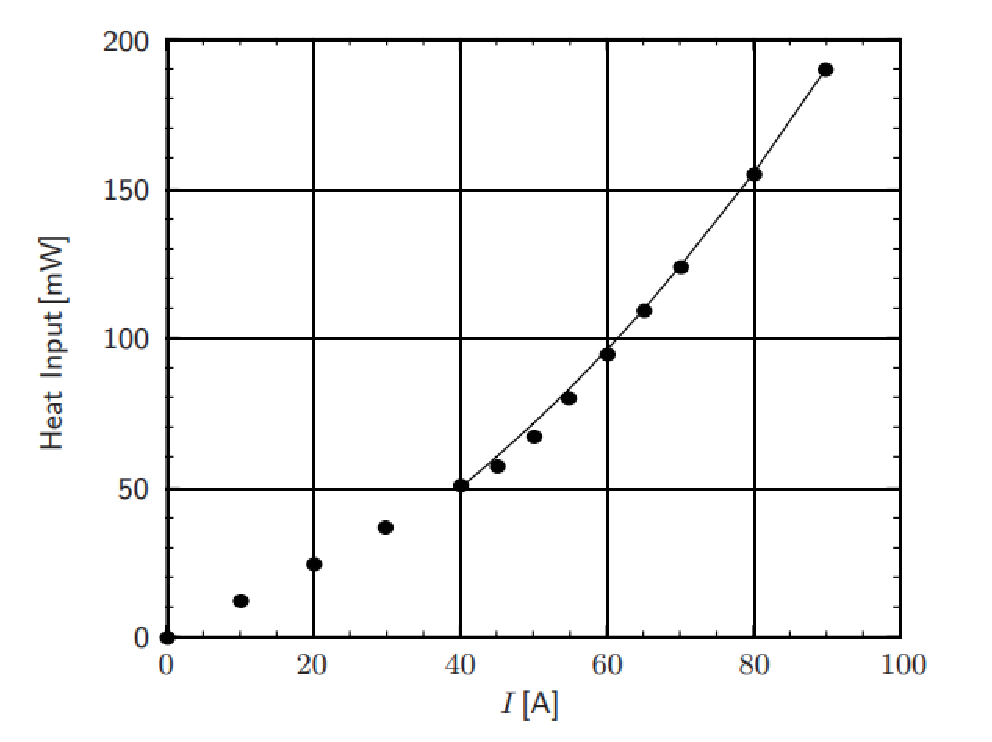
\includegraphics[scale=0.7]{chpt4/figs/fig4.25.eps}
	\caption{。}
\end{figure}

\begin{figure}[htbp]
	\centering
	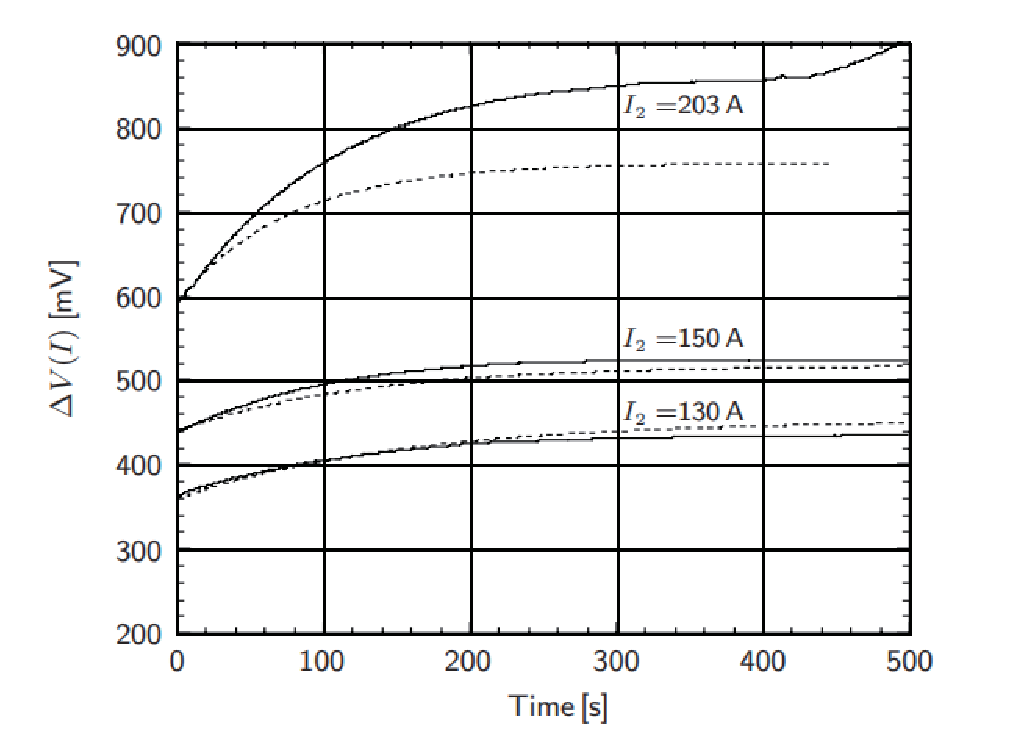
\includegraphics[scale=0.7]{chpt4/figs/fig4.26.eps}
	\caption{。}
\end{figure}


\subsection{讨论4.19:气冷支撑棒}
低温容器内的结构支撑向低温环境带来传导热负荷。
就像讨论4.14中的气冷铜电流引线,氦气可以用于跨越两个温度冷却有效长度
(冷端$T_0$,热端$T_\ell$)$\ell$和横截面为$A$的支撑棒,从而极大的降低传导热损耗。

假设棒材料的热导率是温度无关的,为$\~{k}$;氦和棒之间的传热是理想的
我们可以证明棒在无氦冷却时从$T_\ell$到$T_0$的传导热输入$Q_{\bar{vp}}$与有氦冷却的热输入$Q_{vp}$之比为:
\begin{equation}% 4.114
\frac{Q_{\bar{vp}}}{Q_{vp}}=\frac{c_{p0}(T_\ell-T_0)}{h_L\ln\left[\frac{c_{p0}(T_\ell-T_0)}{h_L}+1\right]}
\end{equation}
我们发现,$\frac{Q_{\bar{vp}}}{Q_{vp}}$与棒的尺寸和热导率无关。
代入$c_{p0}$=6.0 J/g K, $h_L$=20.4 J/g, $T_0$=4 K,$T_\ell$=300 K,方程4.114给出:
\begin{align*}
\frac{Q_{\bar{vp}}}{Q_{vp}}=\frac{(6.0\ \mathrm{J/gK})(296\ \mathrm{K})}{(20.4\ \mathrm{J/g})\ln(88)}=19.4\sim 20
\end{align*}
也就是说,可以通过有效利用冷氦气,能够很大程度的降低通过结构件进入的传导热输入。

\subsection{讨论4.20:低温下的结构材料}
低温应用的结构材料必须承受大的应力,同时在大温区内传递很少的热流。
一个可以用于检验材料适合低温应用的性质是$\tilde{k}/\sigma_U$,
这是温度平均热导率(特定温度区间)和极限拉伸强度的比值。
$Q_{\bar{vp}}$和$Q_{vp}$都正比于$\tilde{k}$。

表4.18给出了G-10、304不锈钢、黄铜、红铜作为结构材料的相关参数值;列入红铜是为了展示它的不适合。
基于$\tilde{k}/\sigma_U$,G-10要比不锈钢好;不过,不锈钢更适宜焊接。

\textcolor{red}{表4.18}